% 若编译失败,且生成 .synctex(busy) 辅助文件,可能有两个原因:
% 1. 需要插入的图片不存在:Ctrl + F 搜索 'figure' 将这些代码注释/删除掉即可
% 2. 路径/文件名含中文或空格:更改路径/文件名即可

% --------------------- 文章宏包及相关设置 --------------------- %
% >> ------------------ 文章宏包及相关设置 ------------------ << %
% 设定文章类型与编码格式
    \documentclass[UTF8]{report}		
    \usepackage{media9}
    %\usepackage{multimedia}
% 本文特殊宏包
    \usepackage{siunitx} % 埃米单位

% 本文特殊宏定义
    \def\Re{\mathrm{Re}\,}
    \def\Im{\mathrm{Im}\,}

% 自定义宏定义
    \def\N{\mathbb{N}}
    \def\F{\mathbb{F}}
    \def\Z{\mathbb{Z}}
    \def\Q{\mathbb{Q}}
    \def\R{\mathbb{R}}
    \def\C{\mathbb{C}}
    \def\T{\mathbb{T}}
    \def\S{\mathbb{S}}
    \def\A{\mathbb{A}}
    \def\I{\mathscr{I}}
    \def\Arg{\mathrm{Arg}\,}
    \def\d{\mathrm{d}}
    \def\p{\partial}


% 导入基本宏包
    \usepackage[UTF8]{ctex}     % 设置文档为中文语言
    \usepackage{hyperref}  % 宏包:自动生成超链接 (此宏包与标题中的数学环境冲突)
    \hypersetup{
        colorlinks=true,    % false:边框链接 ; true:彩色链接
        linkcolor={blue},   % 目录,公式,图表,脚注等内部链接颜色
        citecolor={blue},   % 文献引用颜色
        urlcolor={blue}     % 网页 URL 链接颜色,包括 \href 中的 text
    }
    
    % \usepackage{docmute}    % 宏包:子文件导入时自动去除导言区,用于主/子文件的写作方式,\include{./51单片机笔记}即可。注:启用此宏包会导致.tex文件capacity受限。
    \usepackage{amsmath}    % 宏包:数学公式
    \usepackage{mathrsfs}   % 宏包:提供更多数学符号
    \usepackage{amssymb}    % 宏包:提供更多数学符号
    \usepackage{pifont}     % 宏包:提供了特殊符号和字体
    \usepackage{extarrows}  % 宏包:更多箭头符号
    \usepackage{multicol}   % 宏包:支持多栏 


% 文章页面margin设置
    \usepackage[a4paper]{geometry}
        \geometry{top=1in}  % 1 inch= 2.46 cm, 0.75 inch = 1.85 cm
        \geometry{bottom=1in}
        \geometry{left=0.75in}
        \geometry{right=0.75in}   % 设置上下左右页边距
        \geometry{marginparwidth=1.75cm}    % 设置边注距离(注释、标记等)

% 配置数学环境
    \usepackage{amsthm} % 宏包:数学环境配置
    % theorem-line 环境自定义
        \newtheoremstyle{MyLineTheoremStyle}% <name>
            {11pt}% <space above>
            {11pt}% <space below>
            {}% <body font> 使用默认正文字体
            {}% <indent amount>
            {\bfseries}% <theorem head font> 设置标题项为加粗
            {:}% <punctuation after theorem head>
            {.5em}% <space after theorem head>
            {\textbf{#1}\thmnumber{#2}\ \ (\,\textbf{#3}\,)}% 设置标题内容顺序
        \theoremstyle{MyLineTheoremStyle} % 应用自定义的定理样式
        \newtheorem{LineTheorem}{Theorem.\,}
    % theorem-block 环境自定义
        \newtheoremstyle{MyBlockTheoremStyle}% <name>
            {11pt}% <space above>
            {11pt}% <space below>
            {}% <body font> 使用默认正文字体
            {}% <indent amount>
            {\bfseries}% <theorem head font> 设置标题项为加粗
            {:\\ \indent}% <punctuation after theorem head>
            {.5em}% <space after theorem head>
            {\textbf{#1}\thmnumber{#2}\ \ (\,\textbf{#3}\,)}% 设置标题内容顺序
        \theoremstyle{MyBlockTheoremStyle} % 应用自定义的定理样式
        \newtheorem{BlockTheorem}[LineTheorem]{Theorem.\,} % 使用 LineTheorem 的计数器
    % definition 环境自定义
        \newtheoremstyle{MySubsubsectionStyle}% <name>
            {11pt}% <space above>
            {11pt}% <space below>
            {}% <body font> 使用默认正文字体
            {}% <indent amount>
            {\bfseries}% <theorem head font> 设置标题项为加粗
            {:\\ \indent}% <punctuation after theorem head>
            {0pt}% <space after theorem head>
            {\textbf{#3}}% 设置标题内容顺序
        \theoremstyle{MySubsubsectionStyle} % 应用自定义的定理样式
        \newtheorem{definition}{}

%宏包:有色文本框(proof环境)及其设置
    \usepackage[dvipsnames,svgnames]{xcolor}    %设置插入的文本框颜色
    \usepackage[strict]{changepage}     % 提供一个 adjustwidth 环境
    \usepackage{framed}     % 实现方框效果
        \definecolor{graybox_color}{rgb}{0.95,0.95,0.96} % 文本框颜色。修改此行中的 rgb 数值即可改变方框纹颜色,具体颜色的rgb数值可以在网站https://colordrop.io/ 中获得。(截止目前的尝试还没有成功过,感觉单位不一样)(找到喜欢的颜色,点击下方的小眼睛,找到rgb值,复制修改即可)
        \newenvironment{graybox}{%
        \def\FrameCommand{%
        \hspace{1pt}%
        {\color{gray}\small \vrule width 2pt}%
        {\color{graybox_color}\vrule width 4pt}%
        \colorbox{graybox_color}%
        }%
        \MakeFramed{\advance\hsize-\width\FrameRestore}%
        \noindent\hspace{-4.55pt}% disable indenting first paragraph
        \begin{adjustwidth}{}{7pt}%
        \vspace{2pt}\vspace{2pt}%
        }
        {%
        \vspace{2pt}\end{adjustwidth}\endMakeFramed%
        }

% 外源代码插入设置
    % matlab 代码插入设置
    \usepackage{matlab-prettifier}
        \lstset{
            style=Matlab-editor,  % 继承matlab代码颜色等
        }
    \usepackage[most]{tcolorbox} % 引入tcolorbox包 
    \usepackage{listings} % 引入listings包
        \tcbuselibrary{listings, skins, breakable}
        \newfontfamily\codefont{Consolas} % 定义需要的 codefont 字体
        \lstdefinestyle{matlabstyle}{
            language=Matlab,
            basicstyle=\small\ttfamily\codefont,    % ttfamily 确保等宽 
            breakatwhitespace=false,
            breaklines=true,
            captionpos=b,
            keepspaces=true,
            numbers=left,
            numbersep=15pt,
            showspaces=false,
            showstringspaces=false,
            showtabs=false,
            tabsize=2
        }
        \newtcblisting{matlablisting}{
            arc=2pt,        % 圆角半径
            top=-5pt,
            bottom=-5pt,
            left=1mm,
            listing only,
            listing style=matlabstyle,
            breakable,
            colback=white   % 选一个合适的颜色
        }

% table 支持
    \usepackage{booktabs}   % 宏包:三线表
    \usepackage{tabularray} % 宏包:表格排版
    \usepackage{longtable}  % 宏包:长表格

% figure 设置
    \usepackage{graphicx}  % 支持 jpg, png, eps, pdf 图片 
    \usepackage{svg}       % 支持 svg 图片
        \svgsetup{
            % 指向 inkscape.exe 的路径
            %inkscapeexe = C:/aa_MySame/inkscape/bin/inkscape.exe, 
            inkscapeexe = C:/aa_MySame/inkscape/bin/inkscape.exe,  
            % 一定程度上修复导入后图片文字溢出几何图形的问题
            inkscapelatex = false                 
        }

% 图表进阶设置
    \usepackage{caption}    % 图注、表注
        \captionsetup[figure]{name=图}  
        \captionsetup[table]{name=表}
        \captionsetup{labelfont=bf, font=small}
    \usepackage{float}     % 图表位置浮动设置 
    \usepackage{subcaption} % subfigure 子图支持

% 圆圈序号自定义
    \newcommand*\circled[1]{\tikz[baseline=(char.base)]{\node[shape=circle,draw,inner sep=0.8pt, line width = 0.03em] (char) {\small \bfseries #1};}}   % TikZ solution

% 列表设置
    \usepackage{enumitem}   % 宏包:列表环境设置
        \setlist[enumerate]{
            label=(\arabic*) ,   % 设置序号样式为 (1) (2) (3)
            ref=\arabic*, % 如果需要引用列表项,这将决定引用格式(这里仍然使用数字)
            itemsep=0pt, parsep=0pt, topsep=0pt, partopsep=0pt, leftmargin=3.5em} 
        \setlist[itemize]{itemsep=0pt, parsep=0pt, topsep=0pt, partopsep=0pt, leftmargin=3.5em}
        \newlist{circledenum}{enumerate}{1} % 创建一个新的枚举环境  
        \setlist[circledenum,1]{  
            label=\protect\circled{\arabic*}, % 使用 \arabic* 来获取当前枚举计数器的值,并用 \circled 包装它  
            ref=\arabic*, % 如果需要引用列表项,这将决定引用格式(这里仍然使用数字)
            itemsep=0pt, parsep=0pt, topsep=0pt, partopsep=0pt, leftmargin=3.5em
        }  

% 其它设置
    % 脚注设置
        \renewcommand\thefootnote{\ding{\numexpr171+\value{footnote}}}
    % 参考文献引用设置
        \bibliographystyle{unsrt}   % 设置参考文献引用格式为unsrt
        \newcommand{\upcite}[1]{\textsuperscript{\cite{#1}}}     % 自定义上角标式引用
    % 文章序言设置
        \newcommand{\cnabstractname}{序言}
        \newenvironment{cnabstract}{%
            \par\Large
            \noindent\mbox{}\hfill{\bfseries \cnabstractname}\hfill\mbox{}\par
            \vskip 2.5ex
            }{\par\vskip 2.5ex}

% 文章默认字体设置
    \usepackage{fontspec}   % 宏包:字体设置
        \setmainfont{SimSun}    % 设置中文字体为宋体字体
        \setCJKmainfont[AutoFakeBold=3]{SimSun} % 设置加粗字体为 SimSun 族,AutoFakeBold 可以调整字体粗细
        \setmainfont{Times New Roman} % 设置英文字体为Times New Roman

% 各级标题自定义设置
    \usepackage{titlesec}   
        \titleformat{\chapter}[hang]{\normalfont\huge\bfseries\centering}{第\,\thechapter\,章}{20pt}{}
        \titlespacing*{\chapter}{0pt}{-20pt}{20pt} % 控制上方空白的大小
        % section标题自定义设置 
        \titleformat{\section}[hang]{\normalfont\Large\bfseries}{§\,\thesection\,}{8pt}{}
% subsubsection标题自定义设置
%\titleformat{\subsubsection}[hang]{\normalfont\bfseries}{}{8pt}{}

% --------------------- 文章宏包及相关设置 --------------------- %
% >> ------------------ 文章宏包及相关设置 ------------------ << %

% ------------------------ 文章信息区 ------------------------ %
% ------------------------ 文章信息区 ------------------------ %
% 页眉页脚设置
    \usepackage{fancyhdr}   %宏包:页眉页脚设置
        \pagestyle{fancy}
        \fancyhf{}
        \cfoot{\thepage}
        \renewcommand\headrulewidth{1pt}
        \renewcommand\footrulewidth{0pt}
        \lhead{2024.8 -- 2025.1} 
        \chead{光学笔记(Optics Notes)}    
        \rhead{dingyi233@mails.ucas.ac.cn}
%文档信息设置
    \title{光学笔记\\Optics Notes}
    \author{丁毅\\ \footnotesize 中国科学院大学,北京 100049\\ Yi Ding \\ \footnotesize University of Chinese Academy of Sciences, Beijing 100049, China}
    \date{\footnotesize 2024.8 -- 2025.1}
% ------------------------ 文章信息区 ------------------------ %
% ------------------------ 文章信息区 ------------------------ %

% 开始编辑文章

\begin{document} 
\zihao{5}             % 设置全文字号大小, -4 为小四, 5 为五号

% ------------------------ 封面序言与目录 ------------------------ %
% >> --------------------- 封面序言与目录 --------------------- << %
% 封面
\maketitle\newpage  
\pagenumbering{Roman} % 页码为大写罗马数字
\thispagestyle{fancy}   % 显示页码、页眉等

% 序言
\begin{cnabstract}\normalsize 
    本文为笔者本科时的“光学”课程笔记(Notes of Optics, 2024.8-2025.1)。由于个人学识浅陋,认识有限,文中难免有不妥甚至错误之处,望读者不吝指正,在此感谢。我的邮箱是 dingyi233@mails.ucas.ac.cn。\par
    为了更好地学习光学,建议先跳转至附录部分,了解相关理论知识。\par
\end{cnabstract}
\addcontentsline{toc}{chapter}{序言} % 手动添加为目录

% 目录
\setcounter{tocdepth}{1}                % 目录深度(为1时显示到section)
\tableofcontents                        % 目录页
\addcontentsline{toc}{chapter}{目录}    % 手动添加此页为目录
\thispagestyle{fancy}                   % 显示页码、页眉等 

% 收尾工作
\newpage    
\pagenumbering{arabic} 


% >> --------------------- 封面序言与目录 --------------------- << %
% ------------------------ 封面序言与目录 ------------------------ %

\chapter{光学导言}\thispagestyle{fancy}

\section{光学发展简史(略)}


\section{光的几何传播规律}

\begin{definition}[光传播的基本原理]
光传播的常见基本原理:
\begin{enumerate}
    \item 直线传播:光在均匀介质里沿直线传播 \footnote{对高功率激光,此定律不成立}
    \item 反射定律:光线入射到两种不同的均匀介质的分界面上反射线位于入射面内,反射线和入射线分居法线两侧,反射角等于入射角
    \item 折射定律(斯涅尔定律):折射线位于入射面内,折射线与入射线分居法线两侧,入射角的正弦与折射角的正弦
    之比为一与入射角无关的常数 \footnote{折射率较大的一侧称为光密介质;较小的一侧称为光疏介质}
    \begin{equation}
    n_1\sin i_1 = n_2 \sin i_2
    \end{equation}
    
    \begin{figure}[H]\centering
    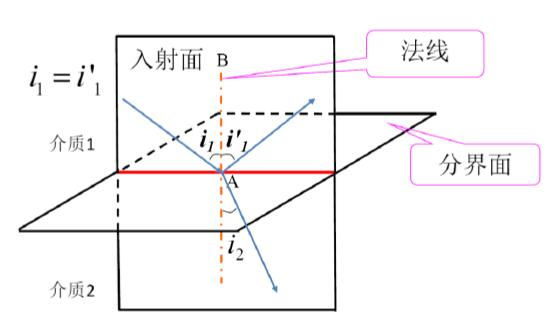
\includegraphics[width=0.4\textwidth]{assets/1,2/image (44).jpg}
    \caption{\textbf{反射与折射}}\label{反射与折射}
    \end{figure}
    
    \item 光路可逆性:光沿反方向传播时,必定沿原光路返回 \footnote{也即在几何光学中,任何光路都是可逆的}
    \item 独立传播:光在传播过程中与其他光束相遇时,各光束都各自独立传播,不改变其传播方向
    \item 全反射:光线从光密介质入射到光疏介质,当入射角大于某临界值时,折射光完
    全消失,只剩下反射光。该临界角度称为全反射临界角。
    \begin{equation}
    i_C = \arcsin (\frac{n_1}{n_2})\quad n_1<n_2
    \end{equation}
\end{enumerate}
\end{definition}


\begin{definition}[彩虹]
\end{definition}


\begin{definition}[三棱镜最小偏向角]

最小偏向角 $\theta_0 = (i_1 - i_1')_{\text{min}}$ 满足:
\begin{equation}
    \theta_0 = 2i_1 - A, \quad \frac{n_2}{n_1} = \frac{\sin\frac{\theta_0+A}2}{\sin\frac A2}
\end{equation}

\begin{figure}[H]\centering
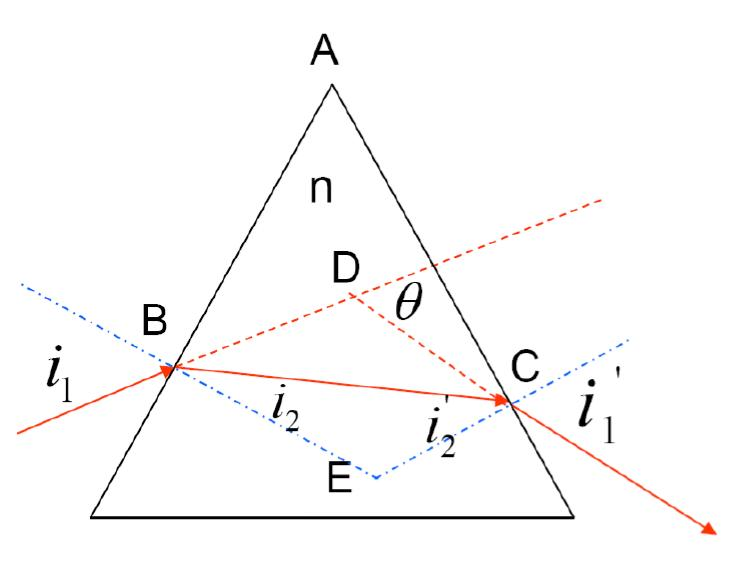
\includegraphics[width=0.4\textwidth]{assets/1,2/image (45).jpg}
\caption{\textbf{三棱镜最小偏向角}}\label{三棱镜最小偏向角}
\end{figure}

\end{definition}

\section{惠更斯原理与费马原理}

\begin{LineTheorem}[惠更斯原理]\label{LineTheorem: 惠更斯原理}
    由振源发出的波动在 $t$ 时刻传播到一个波面 $S$,波面上的每一个面元可认为是次波的波源。由面元发出的次波向四面八方传播。在以后的时刻 $t'$ 形成次波面。这些次波面的包络面 $S'$ 就是 $t'$ 时刻总扰动的波面。
\end{LineTheorem}

\noindent 其中:
\begin{enumerate}
    \item 波面:在同一振源的波场中,扰动同时到达的各点具有相同的相位,这些点的轨迹构成一个曲面,称为波面(也称为等相位面)。
    \item 波线:与波面处处正交的曲线称为波线,其切线方向为光的传播方向
\end{enumerate}

\noindent 几何光学的定律需要前提条件:
\begin{enumerate}
\item 必须是均匀介质,即同一介质的折射率处处相等,折射率不是位置的函数。
\item 必须是各向同性介质,即光在介质中传播时各个方向的折射率相等,折射率不是方向的函数。
\item 光强不能太强,否则巨大的光能量会使线性叠加原理不再成立而出现非线性情况。
\item 光学元件的线度应比光的波长大得多,否则不能把光束简化为光线。
\end{enumerate}

\begin{figure}[H]\centering
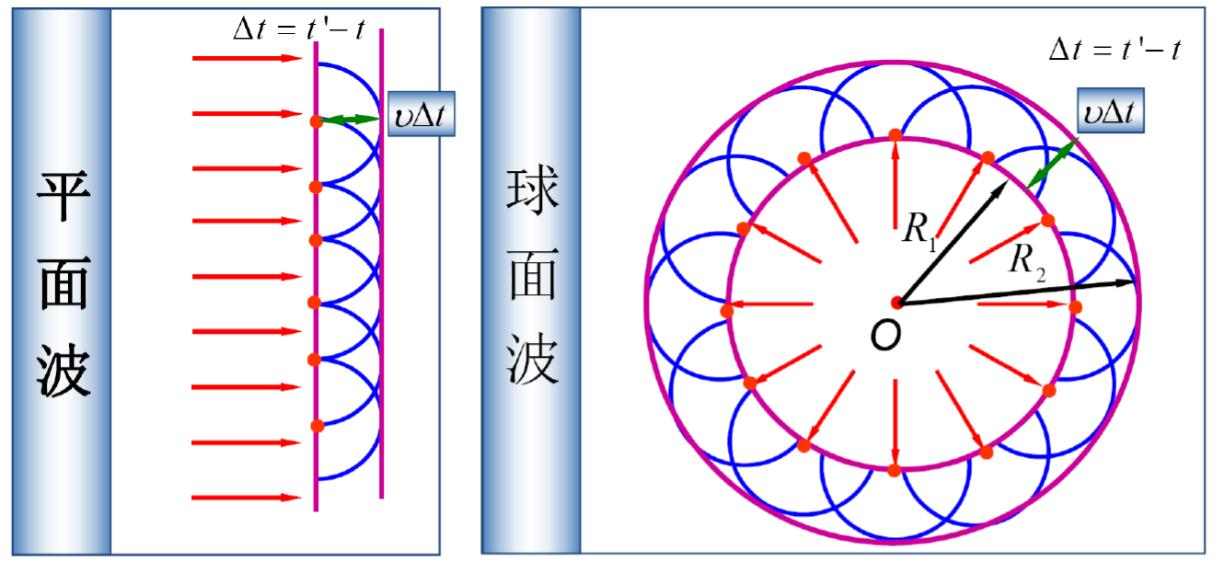
\includegraphics[width=0.5\textwidth]{assets/1,2/image (46).jpg}
\caption{\textbf{惠更斯原理}}\label{惠更斯原理}
\end{figure}

\begin{BlockTheorem}[费马原理]\label{费马原理}
光从空间中一点传播到另一点时,总是沿光程(optical length, OPL)取极值的路径传播 \footnote{这里的“极值”可以是极小值、极大值或常数,一般情况下,实际光程大多取极小值。极大值(如凹面镜成像)、拐点(如椭球面镜、凸透镜)的例子,可以参考 \href{https://zhuanlan.zhihu.com/p/107739173}{知乎:浅谈几何光学(1)——费马原理}},公式:
\begin{equation}
    \mathrm{d}\ \mathrm{OPL} =  \mathrm{d}\left(\int\limits_{Q}^{P}ndl\right)=0 \Longrightarrow \frac{\mathrm{d}\  \mathrm{OPL} }{\mathrm{d} \varphi } = \frac{\mathrm{d} OPL }{\mathrm{d} s } = 0 
\end{equation}
\end{BlockTheorem}
由费马原理可以导出诸多推论,包括我们熟知的几条基本原理,还有物像之间的等光程性(例如凸透镜):
在物点Q与像点Q’之间,不管光线经何路径,凡是由Q通过同样的光学系统到达Q’的光线,都是等光程的。

\section{成像}

理想的像与物体在形状上一致,大小成比例。物与像之间的关系:本质上是一系列物点与像点的点点对应,推广至线线、面面对应。

同心光束:各光线本身或其延长线交于同一点的光束称为同心光束,在各向同性介质中,它对应于球面波。

由若干反射面或折射面组成的光学系统称为光具组

\begin{enumerate}
\item 实物:发散的同心入射光束的“心”
\item 虚物:汇聚的同心入射光束的“心”
\item 实像:发散的同心出射光束的“心”
\item 虚像:汇聚的同心出射光束的“心”
\end{enumerate}

\textbf{物像的共轭性(可逆性):}
若 $P$ 为 物体 $P$(可实可虚)的像点,则反之,当物点为 $P$ 时,像点必在点 $P'$(实际光路可能不同)。是光路可逆性的必然结果。 

计算由物到像的 OPL 时,若为实线(实物、实像)则取正,称为实光程,若为虚线(虚物、虚像)则取负,称为虚光程。

\begin{figure}[H]\centering
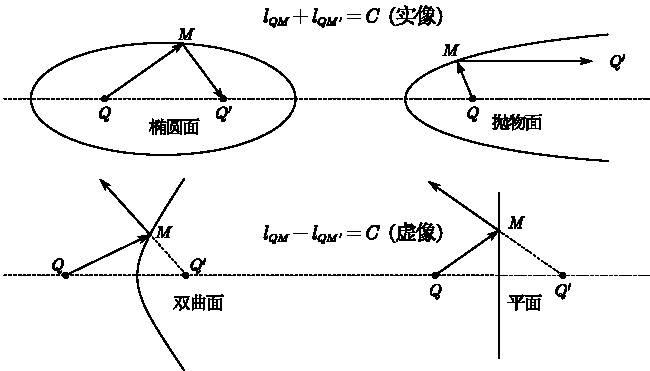
\includegraphics[width=0.7\textwidth]{assets/1,2/path2.pdf}
\caption{\textbf{光程恒定的例子}}\label{光程恒定的例子}
\end{figure}


\begin{definition}[折射球面与反射球面]
的
对于折射球面,存在一对恰好成像的共轭点,称为齐明点。在齐明点处,可以证明 $Q$ 到 $Q'$ 的光程(即物像间的OPL)$l_{QQ'}$。

折射球面公式:
\begin{gather}
\frac{n_1}{l_1} + \frac{n_2}{l_2} = \frac{1}{R\,}\left( \frac{n_{{\color{red} 2}}s_{{\color{red} 2}}}{l_{{\color{red} 2}}} - \frac{n_1s_1}{l_1} \right)
\end{gather}
{\color{gray}\small
\begin{equation}
    \frac{n'}{s'}  +  \frac{n}{s} = \frac{n'-n}{r}\quad  \text{(傍轴)}
\end{equation}
}

反射球面公式:
\begin{equation}
\frac{1}{l_1} + \frac{1}{l_2} = {\color{red} -}\frac{2}{R\,}\left(\frac{s_1}{l_1} + \frac{s_2}{l_2}  \right)
\end{equation}
{\par\color{gray}\small
\begin{equation}
 \frac{1}{s_1} + \frac{1}{s_2} = -\frac{2}{R\,} \quad  \text{(傍轴)}
\end{equation}
\par}

\begin{figure}[H]\centering
\begin{subfigure}[t]{0.45\textwidth}\centering
    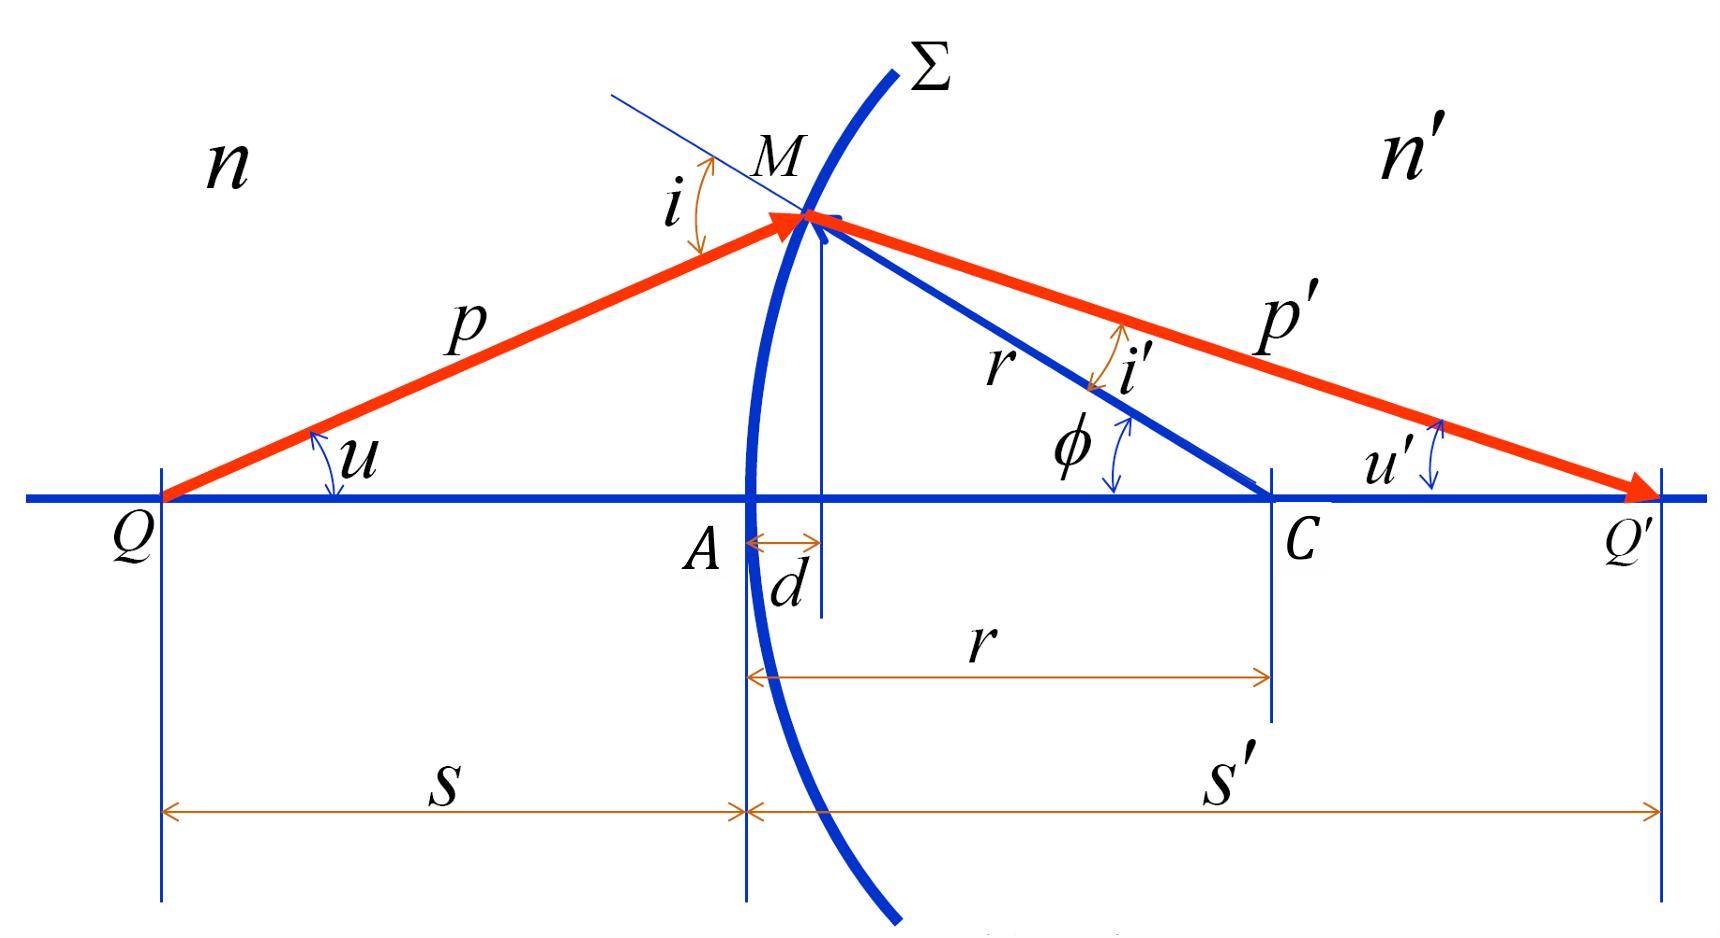
\includegraphics[height=100pt]{assets/1,2/image.jpg}
    \caption{\bfseries 折射球面 }
\end{subfigure}\begin{subfigure}[t]{0.4\textwidth}\centering
    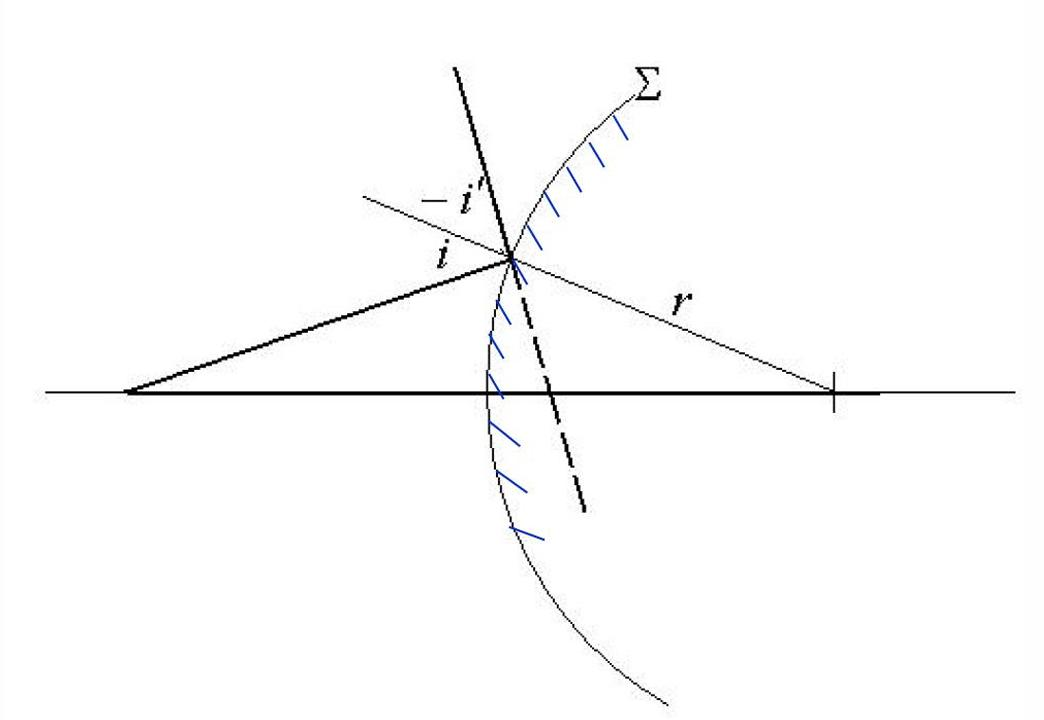
\includegraphics[height=100pt]{assets/1,2/image (1).jpg}
    \caption{\bfseries 反射球面 }
\end{subfigure}
\caption{\bfseries 折射球面与反射球面 }
\end{figure}

\end{definition}


\begin{definition}[像的放大率]
放大率公式:
\begin{equation}
\frac{n_1 | y_1 |}{s_1} = \frac{n_2 | y_2 |}{s_2}
\end{equation}

Lagrange-Helmholtz 恒等式:
\begin{equation}
n_1u_1y_1 = n_2u_2y_2
\end{equation}

上式的 $u$ 和 $y$ 是有正负的,例如折射球面中 $u_1 > 0,\ y_1 >0$ 而 $u_2 <0,\ y_2 < 0$。

\end{definition}





\section{光学仪器}


\subsection{薄透镜}

透镜是由两个共轴折射球面构成的光具组,球面间距远远小于球面半径和物距像距的透镜称为薄透镜,也即 $d \ll | R_1 |, | R_2 |, | s |, | s' |$。此时可以认为两球面顶点重合,称为光心。

薄透镜成像公式(物像距公式):
\begin{gather} 
\frac{n}{s} + \frac{n'}{s'} = \frac{n_L - n}{r_1} + \frac{n' - n_L}{r_2} \label{薄透镜成像公式} \\
s' = \infty \Longrightarrow  f = \frac{n}{\frac{n_L - n}{r_1} + \frac{n' - n_L}{r_2}}\quad \text{物方焦距} \label{物方焦距} \\ 
s = \infty \Longrightarrow  f' = \frac{n'}{\frac{n_L - n}{r_1} + \frac{n' - n_L}{r_2}}\quad \text{像方焦距} \label{像方焦距}
\end{gather}
故物像焦距满足 $\frac{f}{n} = \frac{f'}{n'}$。
特别地,当物像方折射率都为 1 时(真空),我们有磨镜者公式和像的横向放大率:
\begin{equation}
f =f' = \frac{1}{(n_L - 1)(\frac{1}{r_1} - \frac{1}{r_2})},\quad  V = -\frac{\frac{s'}{n'}}{\frac{s}{n}} = -\frac{fs'}{f's} =  - \frac{s'}{s}
\end{equation}


将公式 \ref{物方焦距} 和公式 \ref{像方焦距} 代入式 \ref{薄透镜成像公式} 中,可以得到 Gauss 物像公式:
\begin{equation}
\frac{f}{s} + \frac{f'}{s'} = 1 \overset{n = n'}{\ \ \ \Longrightarrow\ \ \  } \frac{1}{s} + \frac{1}{s'} = \frac{1}{f}
\label{Gauss物像公式}
\end{equation}

令 $s = x + f$,$s' = x' + f'$,代入公式 \ref{Gauss物像公式},可以得到 Newton 物像公式:
\begin{equation}
xx = ff'
\end{equation}


\subsection{其它仪器}
投影仪器、照相机、眼睛、放大镜、显微镜、望远镜

\section{光波的描述}
\section{光度学基本概念}

在学习光度学之前,需要区分辐射度学与光度学中的基本概念。辐射度学研究的是辐射能量对实际物体的影响,而光度学研究的是辐射能量对人眼的影响,是基于人眼实验数据的学科,例如 Luminous Efficiency Function。它们的概念相互对应(可以相互转化)但并不相同,如下表所示: 
\begin{table}[H]\centering
    \caption{\textbf{光度学与辐射度学概念对应关系}}
    \label{光度学与辐射度学概念对应关系}
    \resizebox{\linewidth}{!}{   % 设置宽度为 \linewidth 等比例缩放
    \begin{tabular}{|c|c|c|c|c|c|c|c|}
        \hline
        学科范围 & \multicolumn{7}{c|}{基本概念} \\
        \hline
        辐射度学 & 辐射能 $Q_e$  & 辐射通量 $\Phi_e$  & 辐射强度 $I_e$ & 辐射亮度 $L_e$ &  辐射照度 $E_e$ & 辐射出射度 $M_e$ & 辐射通量谱密度 $\Phi_{e,\lambda}$ \\
        \hline
        光度学   & 光量 $Q_v$ &  光通量 $\Phi_v$  & 光强度 $I_v$ & 光亮度 $L_v$ & 光照度 $E_v$ & 光出射度 $M_v$ & 光通量谱密度 $\Phi_{v,\lambda}$\\
        \hline
    \end{tabular}
    }
\end{table}



\subsection{辐射度学基本概念}

\begin{table}[H]\centering
    \caption{\textbf{辐射度学基本概念}}
    \label{辐射度学基本概念}
    \renewcommand{\arraystretch}{1.1} % 调整行间距为默认值的1.5倍
%\resizebox{0.9\linewidth}{!}{   % 设置宽度为 \linewidth 等比例缩放
%}
\begin{tabular}{|c|c|c|c|c|c|c|c|c|c|}\hline
    名称 & 符号& 定义式 & 单位 & 概念描述\\
    \hline
    辐射能 & $Q_e$ & - & J & 以辐射形式传播的能量 \\
    \hline
    辐通量 & $\Phi_e$ & $\Phi_e = \frac{\mathrm{d}Q_e}{\mathrm{d}t}$ & W & 单位时间内流过某截面的辐射能量 \\
    \hline
    辐强度 & $\boldsymbol{I}_e$ & $\boldsymbol{I}_e = \frac{\mathrm{d}\Phi_e }{\mathrm{d} \boldsymbol{\Omega} } $ & $\mathrm{W\cdot sr^{-1}}$ & 点辐射源在某方向上单位立体角\footnote{立体角的定义参考 \href{https://www.zhihu.com/question/611533175/answer/3244345528}{辐亮度和辐照度是如何计算的}}内的辐射通量 \\
    \hline
    辐照度 & $\boldsymbol{E}_e$ & $ \boldsymbol{E}_e = \frac{\mathrm{d}\Phi_e}{\mathrm{d}\boldsymbol{A}}$ & $\mathrm{W\cdot m^{-2}}$ & 被辐射体单位面积上的辐射通量 \\
    \hline
    辐亮度 & $\boldsymbol{L}_e$ & $\boldsymbol{L}_e = \frac{\mathrm{d}\boldsymbol{I}_e}{\mathrm{d}A \cos \theta} $ & $\mathrm{\mathrm{W}\cdot sr^{-1}\cdot m^{-2}}$ & 单位面积的面辐射源在某方向上的辐射强度\\
    \hline
    辐出射度 & $M_e$ & $ M_e = \frac{\mathrm{d}\Phi_e}{\mathrm{d}A}$ & $\mathrm{W\cdot m^{-2}} $ & 辐射体单位面积向半球空间发射的辐射通量 \\
    \hline
    辐谱密度 & $\phi_e$ & $\phi_e = \frac{\Delta \Phi_{e,\lambda}}{ \Delta\lambda} $ & $\mathrm{W\cdot m^{-1}} $ & 辐射能(通量)在频谱中的分布 \\
    \hline
\end{tabular}
\end{table}

其中 $\Delta \Phi_{e,\lambda}$ 表示波长为 $\lambda$(也可认为是 $[\lambda,\ \lambda + \Delta \lambda]$)的部分所贡献的辐射通量。

\subsection{明视觉曲线}

人眼对不同波长的光具有不同的明亮感觉程度\footnote{参考 \href{https://www.writebug.com/static/uploads/2024/9/16/09153f4fce1d2b99e38c19ef9deeda44.pdf}{新旧明视觉光谱光视效率曲线.pdf}。},称为明视觉光谱光视效率曲线\footnote{参考 \href{https://webstore.ansi.org/preview-pages/ESTA/preview_E1-48_2014.pdf}{ANSI E1.48 - 2014 (A Recommended Luminous Efficiency Function for Stage and Studio Luminaire Photometry)},国际照明委员会(CIE)规定的标准光谱光视效率函数 \href{https://rdrr.io/cran/colorSpec/man/luminsivity.html}{Luminous Efficiency Functions} 或者 \href{https://www.zhihu.com/question/400643965/answer/2727547334}{知乎:光通量与光辐照度之间的换算}。}(函数),常简称为“明视觉曲线”或“视觉曲线”,记为 $V = V(\lambda)$。

光谱光效能 $K$,表示在某一波长上每一瓦辐射通量可以产生多少流明的光通量。光谱光视效率 $V = V(\lambda)$,就是归一化的光谱光效能:
\begin{equation}\label{光谱光效能}
    K = \frac{\Delta \Phi_{v,\lambda}}{\Delta \Phi_{e,\lambda}} = \frac{\phi_v(\lambda)}{\phi_e(\lambda)}, \quad V(\lambda) = \frac{K(\lambda)}{K_{\text{max}}} = \frac{1}{K_{\text{max}}}\cdot \frac{\phi_v(\lambda)}{\phi_e(\lambda)}
\end{equation}
$K_{\text{max}} = 683\ \mathrm{lm \cdot W^{-1}}$ 在波长约 555.0 nm 取到,因此 $V = V(\lambda)$ 也表示在相同辐射通量下,波长为 $\lambda$ 的光与 555.0 nm 的光所产生的亮暗感觉比值。

另外,公式 \ref{光谱光效能} 建立了辐射度学参量与光度学参量之间的转化关系:
\begin{equation}
\Phi_v(\lambda) 
= \int \phi_v(\lambda) \mathrm{d} \lambda 
= \int K_{\text{max}}V(\lambda)\phi_e(\lambda) \mathrm{d} \lambda  
\end{equation}

\subsection{光度学基本概念}

\begin{table}[H]\centering
    \caption{\textbf{光度学基本概念}}
    \label{光度学基本概念}
    \renewcommand{\arraystretch}{1.15} % 调整行间距为默认值的1.5倍
%\resizebox{0.9\linewidth}{!}{   % 设置宽度为 \linewidth 等比例缩放
%}
\begin{tabular}{|c|c|c|c|c|c|c|c|c|c|}\hline
    名称 & 符号& 定义式 & 单位 & 概念描述\\
    \hline
    光量 & $Q_v$ & $Q_v(\lambda) = V(\lambda)\cdot Q_e(\lambda)$ & $\mathrm{cd \cdot sr \cdot s}$ & 辐射能的光度量大小 \\
    \hline
    光通量 & $\Phi_v$ & $\Phi_v = \frac{\mathrm{d}Q_v}{\mathrm{d}t}$ & $\mathrm{lm} = \mathrm{cd \cdot sr}$ & 单位时间内流过某截面的光度学光量 \\
    \hline
    光强度 & $\boldsymbol{I}_v$ & $\boldsymbol{I}_v = \frac{\mathrm{d}\Phi_v }{\mathrm{d} \boldsymbol{\Omega} } $ & $\mathrm{cd}$ & 点辐射源在某方向上单位立体角内的光通量 \\
    \hline
    光照度 & $\boldsymbol{E}_v$ & $ \boldsymbol{E}_v = \frac{\mathrm{d}\Phi_v}{\mathrm{d}\boldsymbol{A}}$ & $\mathrm{lm \cdot m^{-2}}$ & 被辐射体单位面积上的光通量 \\
    \hline
    光亮度 & $\boldsymbol{L}_v$ & $\boldsymbol{L}_v = \frac{\mathrm{d}\boldsymbol{I}_v}{\mathrm{d}A \cos \theta} $ & $\mathrm{cd \cdot m^{-2}}$ & 单位面积的面辐射源在某方向上的光强度 \\
    \hline
    光出射度 & $M_v$ & $ M_v = \frac{\mathrm{d}\Phi_v}{\mathrm{d}A}$ & $\mathrm{lm \cdot m^{-2}} $ & 辐射体单位面积向半球空间发射的光通量 \\
    \hline
    光谱密度 & $\phi_v$ & $\phi_v = \frac{\Delta \Phi_{v,\lambda}}{ \Delta\lambda} $ & $\mathrm{lm \cdot m^{-1}}$ & 光量(光通量)在频谱中的分布 \\
    \hline
\end{tabular}
\end{table}

它们\footnote{参考 \href{https://www.zhihu.com/question/53080536/answer/133398317}{知乎:如何区分并记忆光度、照度、发光强度、光强、亮度等}}之间的转化关系:
\begin{gather}
\text{与光通量的转换:} \Phi_v = \int \boldsymbol{E}_v \mathrm{d}\boldsymbol{A} = \int \boldsymbol{I}_v \mathrm{d}\boldsymbol{\Omega} = \iint \boldsymbol{L}_v \cos \theta\, \mathrm{d}A \,\mathrm{d} \boldsymbol{\Omega} \\ 
\text{与光强的转换:} \boldsymbol{I}_v = r^2\boldsymbol{E}_v = \int \boldsymbol{L}_v \cos \theta\, \mathrm{d}A = \int \boldsymbol{L}_v  \mathrm{d}A_{\perp}
\end{gather}

计算时的常用微分:
\begin{gather}
\begin{aligned}
    & \text{直角坐标系:}&& \mathrm{d}A = \mathrm{d}x \mathrm{d}y &&,  \mathrm{d}\boldsymbol{\Omega} = \frac{\mathrm{d}\boldsymbol{A}}{r^2} \\ 
    & \text{球坐标系:}&& \mathrm{d}A = r^2 \sin \theta \mathrm{d}\theta \mathrm{d}\phi &&,\mathrm{d}\Omega = \sin \theta \mathrm{d}\theta \mathrm{d}\phi \\ 
\end{aligned}
\end{gather}

\section{特殊发光体}

\subsection{余弦发光体(朗伯发光体)}

\subsection{定向发光体}

\chapter{光的反射与折射}\thispagestyle{fancy}

在本章,我们先以一定的顺序,依次对反射折射过程中所出现的现象或相关物理量进行讨论,最后给出所有现象的总结。

\section{菲涅尔公式}

\begin{BlockTheorem}[菲涅尔公式, Fresnel Formula]\label{菲涅尔公式}
光线在通过两介质分界面时通常会同时发生折射(透射)和反射现象,设入射光(incident ray)介质折射率 $\eta_i$,入射角 $\theta_i$,透射光(transmitted ray)介质折射率 $\eta_t$,透射角(折射角)$\theta_t$,则有\footnote{对于金属材质(非绝缘材质),需要引入消光系数 $k_t$ 来修正菲涅尔公式(绝缘材质等价于 $k_t = 0$),具体参见 \href{https://zhuanlan.zhihu.com/p/480405520?utm_psn=1818236176659771392}{知乎: 菲涅尔公式}}:


\begin{table}[H]
\centering
\renewcommand{\arraystretch}{1.6} % 调整行间距为默认值的1.5倍 
\begin{tabular}{|c|c|c|c|c|} 
\hline
类型 & \multicolumn{2}{c|}{振幅反射系数 $r$} & \multicolumn{2}{c|}{振幅透射系数 $t$ }  \\ 
\hline
$s$ 波 & $\displaystyle r_s = \frac{n_i\cos \theta_i - n_t \cos \theta_t}{n_i\cos \theta_i + n_t \cos \theta_t} $ & $\displaystyle  - \frac{\sin (\theta_i - \theta_t) }{\sin (\theta_i + \theta_t)}$ & $\displaystyle t_s  = \frac{2n_i \cos \theta_i}{n_i\cos \theta_i + n_t \cos \theta_t} $ &   $\displaystyle  + \frac{2 \sin \theta_t \cos \theta_i}{\sin (\theta_i + \theta_t)}$   \\ 
\hline
$p$ 波 & $\displaystyle r_p = \frac{n_t\cos \theta_i - n_i \cos \theta_t}{n_t\cos \theta_i + n_i \cos \theta_t} $ &     $ \displaystyle  + \frac{\tan (\theta_i - \theta_t)}{\tan (\theta_i + \theta_t)} $  &  $\displaystyle t_p  = \frac{2n_i \cos \theta_i}{n_i\cos \theta_t + n_t \cos \theta_i} $ &   $\displaystyle + \frac{2 \sin \theta_t \cos \theta_i}{\sin (\theta_i + \theta_t) \cos (\theta_i - \theta_t)}$                  \\
\hline
\end{tabular}
\end{table}

折射角 $\theta_t$、$s$ 波通量反射率 $R_s$、$p$ 波通量反射率 $R_p$ 和总通量反射率 $R$ 为:
\begin{equation}
    \cos \theta_t = \sqrt{1 - \left( \frac{\eta_i}{\eta_t} \sin \theta_i\right)^2},\quad R_s = r_s^2,\ R_p = r_p^2, \quad  R = \frac{1}{2}\left( R_s + R_p \right)
\end{equation}

总强度反射率 $R$ 的严格证明见下一节。特别地,若 $1 - \left( \frac{\eta_i}{\eta_t} \sin \theta_i\right)^2 < 0$,则发生全反射,此时 $R = 1$。另外,需要指出菲涅尔公式的适用条件,也即推导时所做的一些假设,如下:
\begin{enumerate}
\item 介质为绝缘介质,无表面自由电荷或传导电流
\item 介质为各向同性的光学线性介质(弱光强)
\item 介质磁导率(约)等于真空磁导率\footnote{对于介质磁导率不等于真空磁导率的情况,参考 \href{https://www.writebug.com/static/uploads/2024/9/2/3ed06af7e4f074f1964feb480a541a6b.pdf}{Optics (Eugene Hecht, 尤金) Page 144}} $\mu_i = \mu_t = \mu_0$,其中 $\mu_0$ 为真空磁导率。
\end{enumerate}
\end{BlockTheorem}

\section{反射时的相位变化}

菲涅尔公式的推导以矢量分析为基础,因此公式中系数 $r_s$ 的正负具有明确物理意义,它标识着方向。若为负,则反射后的方向与原方向相反,否则相同。各系数正负情况见表 \ref{振幅系数的正负情况},其中 o 表示可正可负。

%\footnote{拓展阅读 \href{https://zhuanlan.zhihu.com/p/607510257}{知乎:你一直没搞懂的半波损失(机械波、光波)}}

\begin{center}\noindent\begin{minipage}{0.65\columnwidth}
    \hspace*{2em} 从波的角度,方向相反可以等价地视为相位发生了 $\pi$ 的前移(或后移),称为相位突变。$n_i < n_t$ 时,相位突变要么是 0,要么是 $\pi$,$n_i > n_t$ 时的相位变化比较复杂,我们不深究。在 $\theta_i + \theta_t = \frac{\pi}{2}$ 时,$r_p$ 的正负发生变化,$p$ 波的反射波相位也发生突变,称此时 $\theta_i$ 的角度为布儒斯特角(Brewster angle),记为 $\theta_B$,也称为偏振角或起偏角。
\end{minipage}\hfill\begin{minipage}{0.3\columnwidth}
    \begin{table}[H]\centering
        % \setlength{\tabcolsep}{1.5mm} % 调整列间距
            \caption{\textbf{振幅系数的正负情况}}
            \label{振幅系数的正负情况}
        \begin{tabular}{cccccccccc}\toprule
            折射率 & $r_s$& $r_p$ & $t_s$ & $t_p$\\
            \midrule                        
            $n_i < n_t$ & $-$ & o & $+$ & $+$\\
            $n_i > n_t$ & o & o & $+$ & $+$\\
            \bottomrule
        \end{tabular}
    \end{table}
\end{minipage}\end{center}
可以推得 Brewster angle 的值为:
\begin{equation}
    \theta_B = \arctan \left( \frac{n_2}{n_1} \right)
\end{equation}



具体的振幅系数变化见图 \ref{振幅系数随入射角的变化},见图 \ref{反射时 s 波和 p 波的相位变化},$n_i < n_t$ 时的反射示意图见图 \ref{反射示意图}。

\begin{figure}[H]\centering
\begin{subfigure}[t]{0.49\textwidth}\centering
    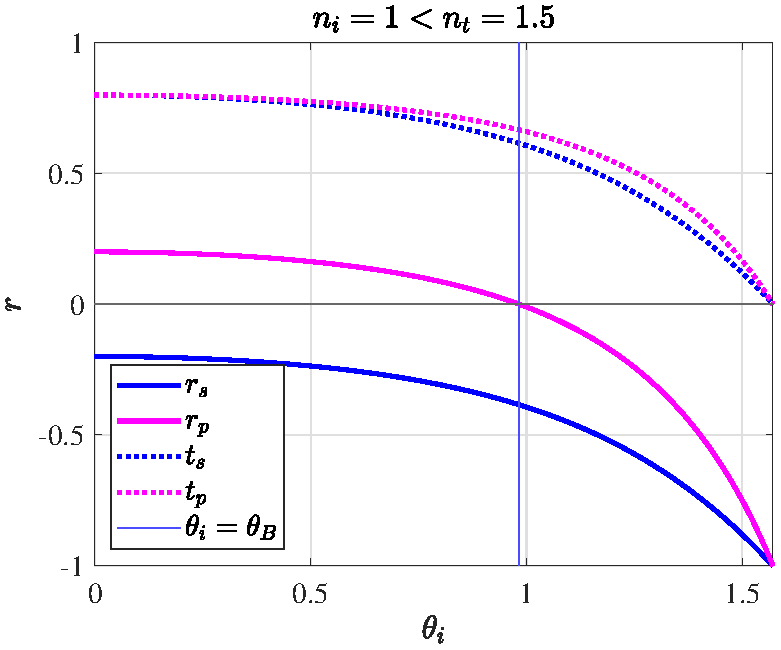
\includegraphics[height=190pt]{assets/1,2/2024-09-15_10-53-31.pdf}
    \caption{\bfseries 由空气入射玻璃($n_i = 1,\ n_t = 1.5$) }
\end{subfigure}
\begin{subfigure}[t]{0.49\textwidth}\centering
    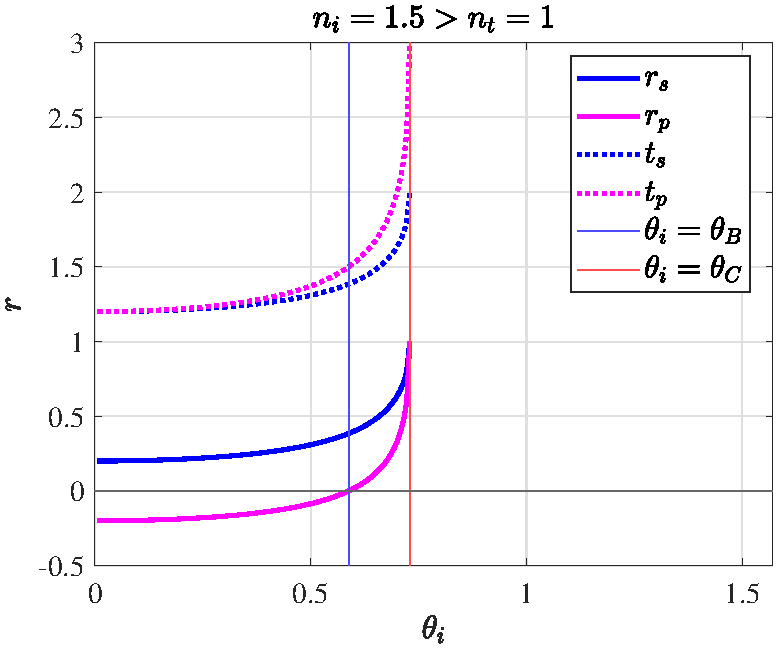
\includegraphics[height=190pt]{assets/1,2/2024-09-15_10-53-27.pdf}
    \caption{\bfseries 由玻璃入射空气($n_i = 1.5,\ n_t = 1$) }
\end{subfigure}
\caption{\bfseries 振幅系数 $r$ 随入射角 $\theta_i$ 的变化 }\label{振幅系数随入射角的变化}
\end{figure}

\begin{figure}[ht]\centering
    \includesvg[width=0.93\textwidth]{assets/1,2/相位突变.svg}
    \caption{\bfseries $s$ 波和 $p$ 波在反射时的相位变化}\label{反射时 s 波和 p 波的相位变化}
\end{figure}

\begin{figure}[H]\centering
\includesvg[width=0.95\textwidth]{assets/1,2/反射后的方向情况.svg}
\caption{\bfseries 由空气入射玻璃的光线示意图}\label{反射示意图}
\end{figure}


由菲涅尔公式,当 $n_i < n_t$ 时,我们还有如下结论:
\begin{gather}
    \begin{aligned}
        &\text{$\theta_i = 0$ 时:} &&r_p = (-r_s)  = \frac{n_t - n_i}{n_t + n_i}, &&t_p = t_s = \frac{2n_i}{n_i + n_t} \\ 
        &\text{$\theta_i = \frac{\pi}{2}$ 时:} &&r_p = r_s  = -1,&&t_p = t_s  =0
    \end{aligned}
\end{gather}
这表明,即使是正射(垂直于介质分界面的入射,$\theta_i = 0$),一般也存在部分反射光。总之,当 $n_i < n_t$ 时,入射光的 s 分量在反射中一定会相位跃变,p 分量都有可能。

另外,菲涅尔公式还可写成:
\begin{gather}
\boxed{
\begin{aligned}
    &\quad\quad \quad \quad   (-r_s) + t_s  = 1, &&\quad 
    \quad \quad\quad   r_p + t_p = 1 
    \\ 
    &r_s = \frac{\cos \theta_i - \sqrt{n_{ti}^2 - \sin^2 \theta_i} }{\cos \theta_i + \sqrt{n_{ti}^2 - \sin^2 \theta_i}}, && r_p = \frac{n_{ti}^2\cos \theta_i - \sqrt{n_{ti}^2 - \sin^2 \theta_i} }{n_{ti}^2\cos \theta_i + \sqrt{n_{ti}^2 - \sin^2 \theta_i}}
\end{aligned}
}
\end{gather}

\section{完全偏振反射光}

当光波由布儒斯特角 $\theta_B$ 入射时,由 Fresnel Formula,$r_p = \frac{\tan (\theta_i - \theta_t)}{\tan (\theta_i + \theta_t)} = 0$,也即反射光的 p 分量为 0,仅存在 s 分量。这说明反射光是完全偏振光,$\boldsymbol{E}$ 的方向(称为振动方向)垂直于入射面。
{\par\color{gray}\small
但此时反射光能量占比 $F$ 很小\footnote{可以使用玻璃片堆得到强度较大的偏振光},例如,空气($n=1$)入射玻璃($n = 1.5$)时,$\theta_B = 56.310^\circ$,$F =0.0740 $;玻璃入射空气时,$\theta_B = 33.690^\circ$,$F =0.0740 $。
\par}

    % \begin{matlablisting}
    % n_i = 1;
    % n_t = 1.5;
    % 
    % theta_B = atan(n_t/n_i);
    % theta_t = @(theta_i) asin(n_i/n_t*sin(theta_i));
    % r_s = @(theta_i, theta_t) - sin(theta_i - theta_t)./sin(theta_i + theta_t);
    % r_p = @(theta_i, theta_t) + tan(theta_i - theta_t)./tan(theta_i + theta_t);
    % F = @(theta_i, theta_t) 0.5*( r_s(theta_i, theta_t)^2 + r_p(theta_i, theta_t)^2 );
    % 
    % theta_i = theta_B;
    % disp(['theta_B = ', num2str(rad2deg(theta_B))])
    % disp(['F = ', num2str(F(theta_i, theta_t(theta_i)))])
    % 
    % %{ 
    % Output:
    % theta_B = 56.3099
    % F = 0.073964
    % %}
    % \end{matlablisting}


\section{反射折射时的能量关系}

在 Fresnel Formula 中可以发现,$r_s^2 + t_s^2 \ne 1$,$r_p^2 + t_p^2 \ne 1$,是能量不守恒了吗?显然不是。那么,反射光和透射光的能量关系是怎样的?这需要借助辐射度学的相关概念。

如图,圆形光束从空气入射到分界面上的一个面元 $\boldsymbol{A}$(界面下是玻璃),以此面元为研究对象。考虑玻印亭矢量 $\boldsymbol{S} = \boldsymbol{E} \times \boldsymbol{B}$,即单位时间内通过单位面积的电磁辐射能量(单位面积辐射功率),于是瞬时辐射照度 $\boldsymbol{E}_e$: 
\begin{equation}
\boldsymbol{E}_e = \boldsymbol{S} = c^2 \varepsilon_0 \boldsymbol{E} \times \boldsymbol{B},\quad  E_e = \varepsilon_0 cE^2 \cdot \sqrt{\frac{\varepsilon_r}{\mu_r}} = \frac{\varepsilon_0 c}{\mu_r}\cdot  nE^2
\end{equation}
其中 $\varepsilon_r$,$\mu_r$ 分别为相对介电常量、相对磁导率,对空气近似有 $\varepsilon_r = \mu_r = 1$,于是

核心思想是 $\mathrm{d} Q_e = (\boldsymbol{E}_e \cdot \boldsymbol{A})\, \mathrm{d}t $。入射、反射、透射光束的截面面积分别为 $A \cos \theta_i,\ A \cos \theta_r,\ A \cos \theta_t$,设其瞬时辐射照度分别为$\boldsymbol{E}_i,\ \boldsymbol{E}_r,\ \boldsymbol{E}_t$ ,则辐射通量为:
\begin{equation}
\Phi_{e, k} = E_{e, k} A \cos \theta_k = \frac{\varepsilon_0 cA }{\mu_r}\cdot  n_k\cos \theta_k\,E_k^2,\quad  k = i, r, t
\end{equation}

分别写出入射、反射、透射光的辐射通量:
\begin{align}
\Phi_{e,i} &= \frac{\varepsilon_0 cA }{\mu_r} \cdot  n_i\cos \theta_i\,E_i^2 
= \frac{\varepsilon_0 cA }{\mu_r} \cdot  n_i\cos \theta_i\, \left( E_{i,s}^2 + E_{i,p}^2 \right) 
\\ 
\Phi_{e,r} 
&= \frac{\varepsilon_0 cA }{\mu_r} \cdot  n_i\cos \theta_i\,E_r^2 
= \frac{\varepsilon_0 cA }{\mu_r} \cdot  n_i\cos \theta_i\, \left( r_s^2E_{i,s}^2 + r_p^2E_{i,p}^2 \right) 
\\ 
\Phi_{e,t} 
&= \frac{\varepsilon_0 cA }{\mu_r} \cdot  n_t\cos \theta_t\,E_t^2 
= \frac{\varepsilon_0 cA }{\mu_r} \cdot  n_t \cos \theta_t \, \left( t_s^2E_{i,s}^2 + t_p^2E_{i,p}^2 \right) 
\end{align}

由于入射光可分解为 $s$ 波与 $p$ 波,我们自然想到它们俩在入射前后应该是能量守恒的,这指导我们分别作数学上的处理。对 $s$ 波,由菲涅尔定律(这说明已经做了近似 $\mu_r = 1$),做减法得到:
\begin{align*}
&n_i \cos \theta_i E_{i,s}^2 - n_i \cos \theta_i r_{i,s}^2E_{i,s}^2 -   n_t \cos \theta_t t_s^2E_{i,s}^2 \\
&= E_{i,s}^2 \left[ n_i\cos \theta_i \left( 1 - \frac{(n_i\cos \theta_i - n_t \cos \theta_t)^2}{(n_i\cos \theta_i + n_t \cos \theta_t)^2} \right) - n_t \cos \theta_t \cdot \frac{(2n_i \cos \theta_i)^2}{(n_i\cos \theta_i + n_t \cos \theta_t)^2} \right] \\ 
& = \frac{E_{i,s}^2}{(n_i\cos \theta_i + n_t \cos \theta_t)^2} \left[ n_i \cos \theta_i \cdot (4 n_i\cos \theta_i \cdot n_t \cos \theta_t) - 4 n_t \cos \theta_t \cdot n_i^2 \cos^2 \theta_i\right] \\ 
& = 0
\end{align*}

同理,考虑 p 分量,作减法可得到:
\begin{equation}
n_i \cos \theta_i E_{i,p}^2 - n_i \cos \theta_i r_{i,p}^2E_{i,p}^2 -   n_t \cos \theta_t t_p^2E_{i,p}^2 = 0
\end{equation}

代入即得:
\begin{equation}
    \Phi_{e,i} - \Phi_{e,r} - \Phi_{e,t} = 0 \Longrightarrow  \Phi_{e,i} = \Phi_{e,r} + \Phi_{e,t}
\end{equation}
这便验证了入射前后的能量是守恒的。

由此,我们可以定义一些能量系数:
\begin{gather}
\begin{aligned}
    &\text{强度反射率 $R$: }\ &&R = \frac{1}{2}(R_s + R_p), &&R_s = r_s^2, && R_p = r_p^2 \\
    &\text{强度透射率 $T$: }\ &&T = \frac{1}{2}(T_s + T_p), &&T_s = \left( \frac{n_t \cos \theta_t}{n_i \cos \theta_i} \right)^2 t_s^2, && T_p = \left( \frac{n_t \cos \theta_t}{n_i \cos \theta_i} \right)^2 t_p^2 \\
\end{aligned}
\end{gather}

这样,它们具有下面的性质,方便我们计算能量关系:
\begin{gather}
\boxed{
\begin{aligned}
    &R_s + T_s = 1, &&\quad  R_p + T_p = 1,&&\ \  R + T = 1 \\ 
    &\Phi_{e,r} = R\Phi_{e,i}, && 
    \Phi_{e,r,s} = R_s\Phi_{e,i,s}, &&  \Phi_{e,r,p} = R_p\Phi_{e,i,s} 
    \\ 
    &\Phi_{e,t} = T\Phi_{e,i}, && \Phi_{e,t,s} = T_s\Phi_{e,i,s}, && \Phi_{e,t,p} = T_p\Phi_{e,i,s}
\end{aligned}
}
\end{gather}
{\color{red} 其中 $\Phi_{e,r} = R\Phi_{e,i}$ 和 $\Phi_{e,t} = T\Phi_{e,i}$ 是怎么来的?}




\section{全反射时的隐失波与穿透深度}

假设现在由光密介质射向光疏介质,即 $n_i > n_t$,则有临界角 $\theta_C = \arcsin n_{ti}$。当 $\theta_i > \theta_C$ 时,发生全反射,$R = 1,\ T = 0$,若简单地认为没有任何透射光,是不满足电磁场边界条件的。具体来讲,$\boldsymbol{E}$ 的切向分量连续告诉我们,在透射介质中一定存在振荡场,它在平行于界面上的分量具有时间频率 $\omega$(与入射光相同)。

进一步的推导表明\footnote{详见参考文献 \cite{Optics} 的 Page 158},在透射介质中存在一种波(称为隐失波),其波函数如下:
\begin{equation}
\boldsymbol{E} = \left( e^{-\beta y} \boldsymbol{E_{t,0}}\right)\cdot e^{i\left( \frac{\sin \theta_i}{n_{ti}}  k_t x - \omega t \right)},\quad \text{衰减系数}\  \beta = k_t \sqrt{\frac{\sin^2 \theta_i}{n_{ti}^2} - 1} = k_i\sqrt{\sin^2 \theta_i - n_{ti}^2} 
\end{equation}

这是一个不均匀波,其振幅在 $y$ 方向上极速衰减,只在几个波长的距离上就可以忽略不计。且它同时有纵波成分和横波成分,不是简单的简谐横波。

我们将振幅下降到 $\frac{1}{e}$ 的深度称为\textbf{穿透深度},记为 $\delta = \frac{1}{\beta} $,它通常在一个波长以内。

对于此过程的能量守恒问题,更详尽广泛的讨论表明(利用波印廷矢量 $\boldsymbol{S}$),能量实际上是跨过界面往复循环,最终使透向第二介质的净流量为零。就现阶段,可以理解为能量从入射波流到隐失波再回到反射波,或者说隐失波沿入射波又绕回了反射波。

\section{古斯-亨欣位移(Goos-Hanchen Shift)}

一束被全反射的光,入射点会与(反射后的)出射点存在微小偏移(事实上既有平行偏移也有垂直偏移),称为 Goos-Hanchen Shift。较为严谨的推导表明\footnote{详见参考文献 \cite{GHShift},或者 \href{https://www.zhihu.com/question/446676895/answer/3407740051}{知乎:古斯汉欣位移产生的原因 (https://www.zhihu.com/question/446676895/answer/3407740051)},以及 \href{https://www.zhihu.com/question/620522351/answer/3209865128}{知乎:古斯汉森位移的原理是什么 (https://www.zhihu.com/question/620522351/answer/3209865128)}},沿入射方向、与分界线平行的偏移量如下(又称为侧向偏移):
\begin{equation}
\delta_{\perp} = \frac{\lambda_i \sin \theta_i}{\pi \sqrt{\sin^2 \theta_i - n_{ti}^2} },\quad \Delta x =  \frac{\lambda_i \tan \theta_i}{\pi \sqrt{\sin^2 \theta_i - n_{ti}^2} } = 2 \delta \tan \theta_i 
\end{equation}

\begin{figure}[H]\centering
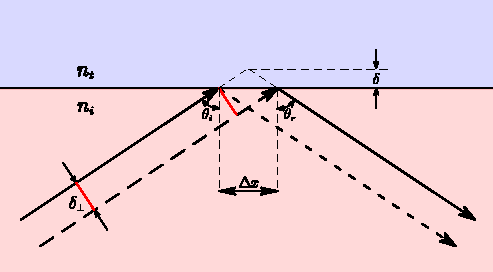
\includegraphics[width=0.8\columnwidth]{assets/1,2/GHShift.pdf}
\caption{\bfseries Goos-Hanchen Shift}\label{Goos-Hanchen Shift}
\end{figure}

\section{全反射时的相位变化}\label{全反射时的相位变化}


发生全内反射时\footnote{全内反射是指,由光疏介质射向光密介质且入射角大于临界角时发生的全反射现象},入射波 s 分量、p 分量的相位变化并非简单的 0 或 $\pi$,下面作推导。

对入射光的波函数 $\boldsymbol{E_i} = \boldsymbol{E_{i,0}} \cdot e^{i \theta} =\boldsymbol{E_{i,0}} \cdot e^{i(k x - \omega t)}$,若反射光满足 $\boldsymbol{E_{r}} = \boldsymbol{E_i}\cdot \lambda e^{i \delta}$,则表明相对于入射光,反射光的振幅变为了原来的 $\lambda$倍,且相位增加了 $\delta$。特别地,$\lambda < 0$ 时,可以等价于 $\lambda > 0$ 且相位增加 $\delta + \pi$ 或 $\delta - \pi$。

由菲涅尔定律,我们有 $\boldsymbol{E_{r,s}} = r_s \boldsymbol{E_{i,s}},\quad \boldsymbol{E_{r,p}} = r_p \boldsymbol{E_{i,p}}$。可以发现,在全反射时,$r_s, r_p \in \C \setminus \R$,并且 $| r_s | = | r_p | = 1$,振幅不变,于是可以令 $r = e^{i \delta }$。为了反解相位增量 $\delta $,一种自然的想法是考虑 
\begin{equation}
    e^{i \delta} = \cos \delta + i \lambda \sin \delta = a + ib \Longrightarrow  \delta =  \arctan \left( \frac{b}{a} \right)
\end{equation}

这样做虽然可行,但由于 $\arctan $ 函数的局限性,其值域范围在 $[-\frac{\pi}{2}, \frac{\pi}{2}]$,而 $\delta $ 的取值范围在 $[0, \pi]$ 或者 $[-\pi, 0]$。因此,最终得到的 $\delta$ 仅在部分区域上正确,对另一部分需做数学上的平移修正。因此,我们考虑另一种方法。在全反射时,注意到 $r_s$ 和 $r_p$ 的形式为 $r = \frac{a - bi}{a +bi}$,其中 $a, b \in \R$,有如下过程:
\begin{equation}
\frac{a - bi}{a + bi} = e^{i \theta} \Longrightarrow e^{i \frac{\theta}{2}} = \pm \frac{a - bi}{\sqrt{a^2 + b^2} },\ \tan \frac{\delta}{2} = - \frac{b}{a},\ \frac{\delta}{2} = \arctan \left( - \frac{b}{a} \right)
\end{equation}
这样得到的 $\frac{\delta}{2}$ 便是全范围正确的,无需修正。分别令 $r = r_s, r_p$,代入即得:
\begin{gather}
\delta_{r,s} = - 2 \arctan \left( \frac{\sqrt{\sin^2 \theta_i - n_{ti}^2} }{\cos \theta_i} \right) 
,\quad 
\delta_{r,p} = - 2 \arctan \left( \frac{\sqrt{\sin^2 \theta_i - n_{ti}^2} }{n_{21}^2 \cos \theta_i} \right)
\end{gather}

\section{折射时的相位变化}

入射光不发生全反射时,由菲涅尔定律,$t_s, t_p \in (0, \frac{2n_i}{n_i + n_t}) \subset \R$,恒为正实数,因此相位不发生任何变化。当入射光发生全反射时,折射光(透射光)以隐失波的形式存在,我们前面已经提过,隐失波同时含有横波纵波成分,它与入射光不再是同一种波,此时谈论相位变化自然没有意义。


\section{反射折射总结}

到此,我们已经讨论了目前可能接触到的所有情况,包括光疏射向光密、光密射向光疏、小于或大于临界角时的折射反射振幅、相位以及能量关系等,终于可以给出反射折射的总结。

整个结论由菲涅尔定律推导而来,基于电磁场的边界条件和麦克斯韦方程组,从波的角度揭示了光在反射折射时发生的变化,包括振幅、相位、能量、位移等关系。
\begin{align}
&\text{反射波:} \quad \boldsymbol{E_r} = \boldsymbol{E_{r,s}} + \boldsymbol{E_{r,p}} = r_s \boldsymbol{E_{i,s}} + r_p \boldsymbol{E_{i,p}},\quad  r \in \C 
\\ 
&\text{透射波:}\quad \boldsymbol{E_t} = \boldsymbol{E_{t,s}} + \boldsymbol{E_{t,p}} = t_s \boldsymbol{E_{i,s}} + t_p \boldsymbol{E_{i,p}},\quad  t \in \R,\ \theta_i < \theta_C
\\ 
& \text{反射系数:}
    r_s = \frac{\cos \theta_i - \sqrt{n_{ti}^2 - \sin^2 \theta_i} }{\cos \theta_i + \sqrt{n_{ti}^2 - \sin^2 \theta_i}},\quad  r_p = \frac{n_{ti}^2\cos \theta_i - \sqrt{n_{ti}^2 - \sin^2 \theta_i} }{n_{ti}^2\cos \theta_i + \sqrt{n_{ti}^2 - \sin^2 \theta_i}}
\\ 
& \text{透射系数:}(-r_s) + t_s  = 1,\quad r_p + t_p = 1 
\\
& \text{能量关系:}
\begin{cases}
    R = \frac{1}{2}(R_s + R_p)\quad R_s = | r_s |^2,\ R_p = | r_p |^2 \\ 
    T = \frac{1}{2}(T_s + T_p),\quad 
    T_s = \left( \frac{n_t \cos \theta_t}{n_i \cos \theta_i} \right)^2 t_s^2, T_p = \left( \frac{n_t \cos \theta_t}{n_i \cos \theta_i} \right)^2 t_p^2 \\
    R + T = 1 ,\ R_s + T_s = 1,\ R_p + T_p = 1 \\ 
    \Phi_{e,r} = R\Phi_{e,i},\ \Phi_{e,t} = T\Phi_{e,i}
\end{cases}
\\
& \text{$s$ 波反射相位增量:} 
\delta_{r,s} = 
\left\{\begin{matrix}
    -\pi, & n_i < n_t \\ 
    \begin{Bmatrix}
        0, & \theta_i \in (0, \theta_C)\\
        - 2 \arctan \left( \frac{\sqrt{\sin^2 \theta_i - n_{ti}^2} }{\cos \theta_i} \right), & \theta_i > \theta_C
    \end{Bmatrix}, & n_i > n_t
\end{matrix}\right.
\\
& \text{$p$ 波反射相位增量:} 
\delta_{r,p} = 
\left\{\begin{matrix}
    \begin{Bmatrix}
        0, & \theta_i \in (0, \theta_B) \\
        - \pi & \theta_i \in (\theta_B, \frac{\pi}{2})
    \end{Bmatrix}, & n_i < n_t 
    \\ 
    \begin{Bmatrix}
        -\pi, & \theta_i \in (0, \theta_B) \\
        0, & \theta_i \in (\theta_B, \theta_C) \\
        - 2 \arctan \left( \frac{\sqrt{\sin^2 \theta_i - n_{ti}^2} }{n_{ti}^2 \cos \theta_i} \right), & \theta_i \in (\theta_C, \frac{\pi}{2})
    \end{Bmatrix}, & n_i > n_t
\end{matrix}\right.
\\
&\text{隐失波:} \boldsymbol{E_{t}} = \left( e^{-\beta y} \boldsymbol{E_{t,0}}\right)\cdot e^{i\left( \frac{\sin \theta_i}{n_{ti}}  k_t x - \omega t \right)},\quad \beta  = k_i\sqrt{\sin^2 \theta_i - n_{ti}^2} = \frac{2 \pi}{\lambda_i} \sqrt{\sin^2 \theta_i - n_{ti}^2},\quad \delta = \frac{1}{\beta}
\\ 
& \text{Goos-Hanchen Shift: \ } \Delta x = 2 \delta \tan \theta_i = \frac{2 \tan \theta_i}{k_i\sqrt{\sin^2 \theta_i - n_{ti}^2}}
= \frac{\lambda_i \tan \theta_i }{\pi \sqrt{\sin^2 \theta_i - n_{ti}^2} }
\end{align}

另外,如图 \ref{光路可逆性下的振幅与能量系数} 考虑一束光由光疏介质射向光密介质($n_i < n_t$),发生透射、反射。保持各角度不变,将透射光方向置反,射向光疏介质,由菲涅尔公式,可得对称前后的振幅与能量系数变化:
\begin{gather}
\theta_i < \theta_B:\ \begin{cases}
    \text{反射振幅与强度:}&\displaystyle \frac{r_s'}{r_s} = \frac{r_p'}{r_p} = 1, \quad \frac{R'}{R} = \frac{R_s'}{R_s} = \frac{R_p'}{R_p} = 1 \\
    \text{透射振幅与强度:} &\displaystyle \frac{t_s'}{t_s} = \frac{t_p'}{t_p} = \frac{\tan A}{\tan B} ,\quad  \frac{T'}{T} = \frac{T_s'}{T_s} = \frac{T_p'}{T_p} = \frac{1}{n_{ti}^2}\cdot \frac{\sin^2 2A}{\sin^2 2B}
\end{cases} \quad 
\\ 
\theta_i > \theta_B:\ \begin{cases}
    \text{反射振幅与强度:}&\displaystyle \frac{r_s'}{r_s} = \frac{r_p'}{r_p} = 1, \quad \frac{R'}{R} = \frac{R_s'}{R_s} = \frac{R_p'}{R_p} = 1 \\
    \text{透射振幅与强度:} &\displaystyle \frac{t_s'}{t_s} = \frac{t_p'}{t_p} = \frac{\tan A}{\tan B} ,\quad  \frac{T'}{T} = \frac{T_s'}{T_s} = \frac{T_p'}{T_p} = \frac{1}{n_{ti}^2}\cdot \frac{\sin^2 2A}{\sin^2 2B}
\end{cases} \quad 
\end{gather}

\begin{figure}[H]\centering
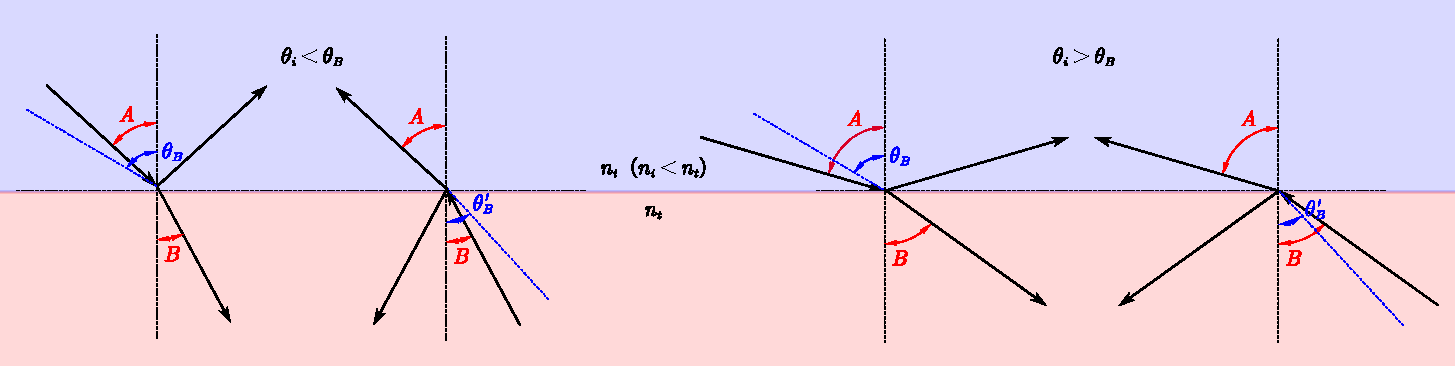
\includegraphics[width=\columnwidth]{assets/3/光路可逆性下的振幅与能量系数.pdf}
\caption{\bfseries 光路可逆性下的振幅与能量系数}\label{光路可逆性下的振幅与能量系数}
\end{figure}

图 \ref{反射折射光的振幅与能量变化} 展示了反射折射光的振幅 $r_s, r_p, t_s, t_p$、能量 $R_s, R_p, R$ 随入射角 $\tan \theta_i$ 的变化\footnote{源码见附录 \ref{反射折射光的振幅与能量变化 源码}},其中 (a) 图为空气入射玻璃($n_i = 1, n_t = 1.5$),(b) 图为玻璃入射空气($n_i = 1.5, n_t = 1$)。

图 \ref{反射光 s 分量与 p 分量的相位增量} 展示了反射光的 s 分量与 p 分量的相位增量 $\delta_{r,s}, \delta_{r,p}$ 随入射角 $\theta_i$ 的变化\footnote{源码见附录 \ref{反射光 s 分量与 p 分量的相位增量 源码}},其中 (a) 图为空气入射玻璃($n_i = 1, n_t = 1.5$),(b) 图为玻璃入射空气($n_i = 1.5, n_t = 1$)。特别地,当 (b) 图中 $\theta_i > \theta_C$ 时,发生全(内)反射,此时 $r_s, r_p, t_s, t_p \in \C \setminus \R$ ,图中展示的是它们的模长,即 $|r_s|, |r_p|, |t_s|, |t_p|$。

图 \ref{隐失波穿透深度与 GH Shift 玻璃入射空气} 展示了隐失波穿透深度 $\delta$ 和 GH SHift $\Delta x$ 随入射角 $\theta_i$ 的变化\footnote{源码见附录 \ref{隐失波穿透深度与 GH Shift 玻璃入射空气 源码}}。


\newpage
\begin{figure}[H]\centering
\begin{subfigure}[t]{0.44\columnwidth}\centering
    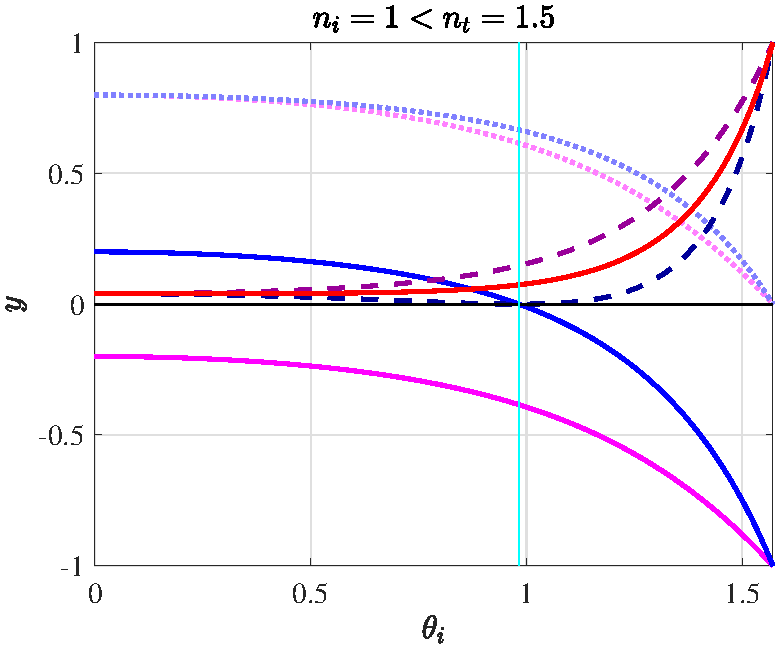
\includegraphics[height=170pt]{assets/1,2/2024-09-21_12-26-37.pdf}
    \caption{\bfseries 由空气入射玻璃 }
\end{subfigure}
\subcaptionsetup{
    margin={2cm,0cm}, % 右边距不变,左边距为 2cm
    %labelsep=period % 标签与标题内容之间的分隔符为点号
    }
\begin{subfigure}[t]{0.54\columnwidth}\centering
    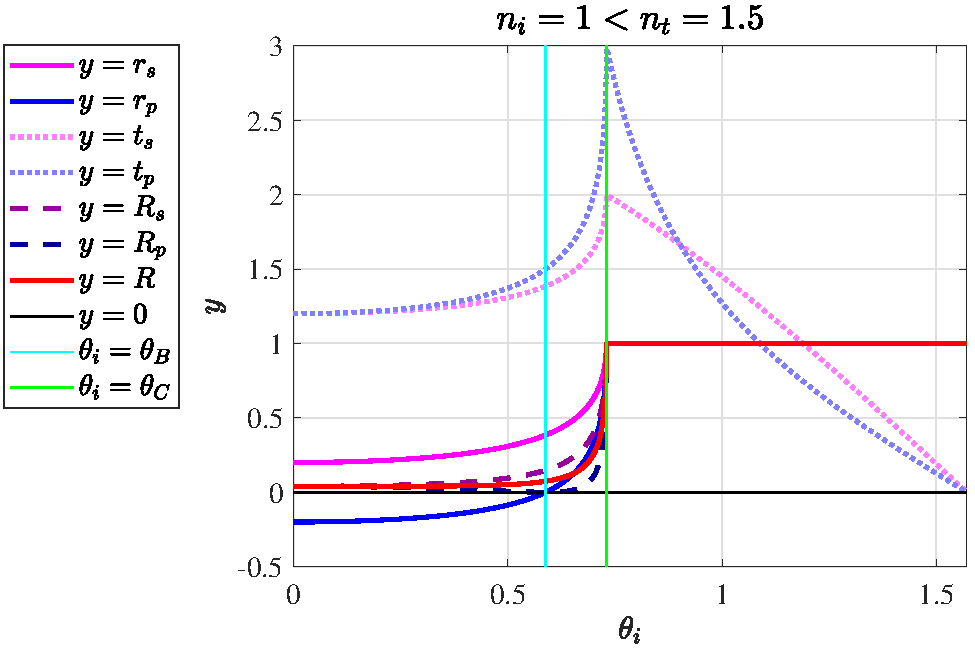
\includegraphics[height=170pt]{assets/1,2/2024-09-21_12-31-00.pdf}
    \caption{\bfseries 由玻璃入射空气 }
\end{subfigure}
\caption{\bfseries 反射折射光的振幅与能量变化 }
\label{反射折射光的振幅与能量变化}
\end{figure}

\begin{figure}[H]\centering
\begin{subfigure}[t]{0.5\columnwidth}\centering
    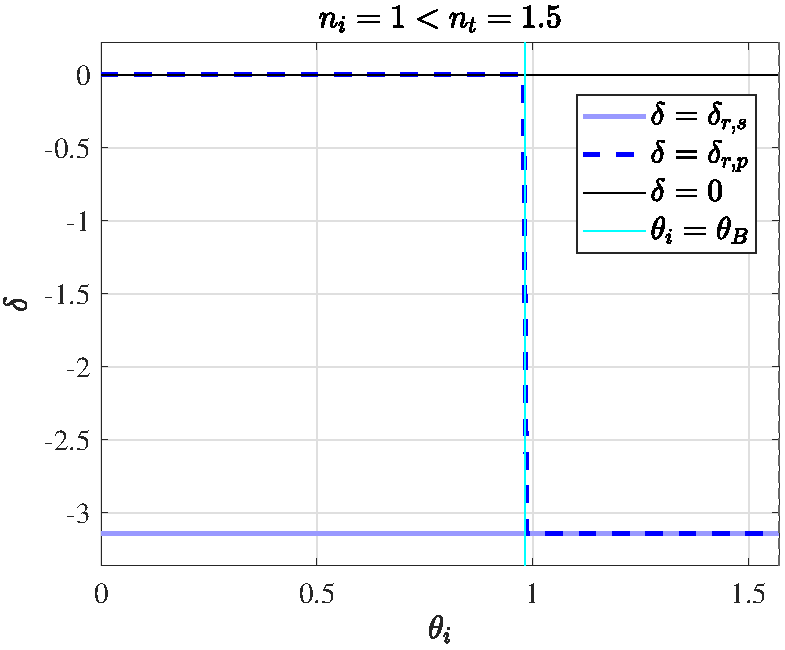
\includegraphics[height=175pt]{assets/1,2/2024-09-21_13-19-43.pdf}
    \caption{\bfseries 由空气入射玻璃 }
\end{subfigure}\begin{subfigure}[t]{0.5\columnwidth}\centering
    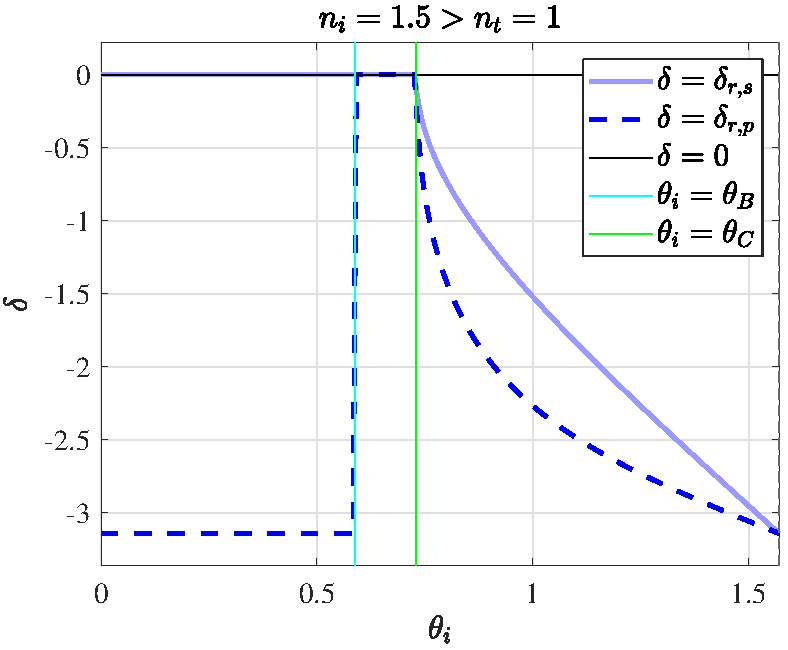
\includegraphics[height=175pt]{assets/1,2/2024-09-21_13-19-45.pdf}
    \caption{\bfseries 由玻璃入射空气 }
\end{subfigure}
\caption{\bfseries 反射光 s 分量与 p 分量的相位增量 }
\label{反射光 s 分量与 p 分量的相位增量}
\end{figure}

\begin{figure}[H]\centering
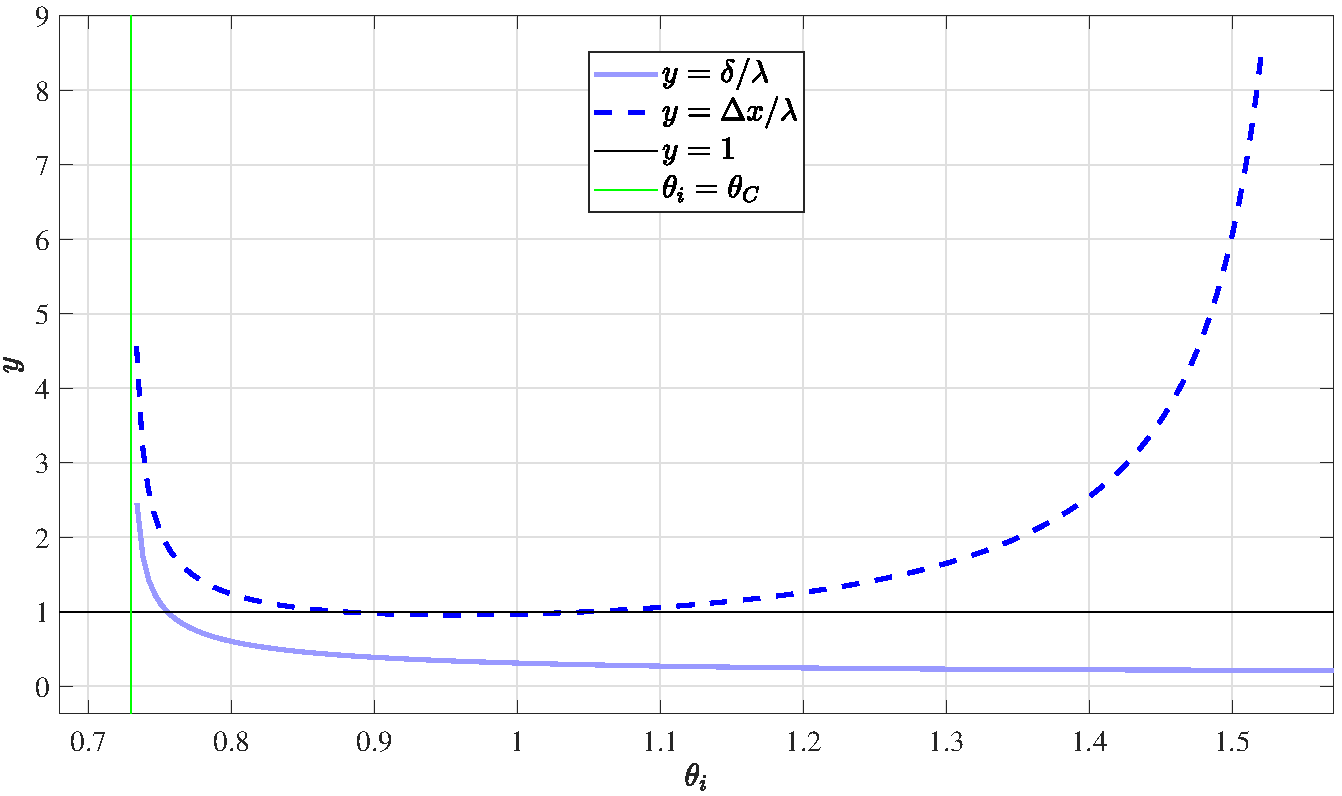
\includegraphics[width=0.70\columnwidth]{assets/1,2/2024-09-21_13-29-49.pdf}
\caption{\bfseries 隐失波穿透深度与 GH Shift(玻璃入射空气)}\label{隐失波穿透深度与 GH Shift 玻璃入射空气}
\end{figure}


\chapter{光的干涉}\thispagestyle{fancy}


通常将平面波与球面波\footnote{即平面电磁波与球面电磁波,详见附录 \ref{平面波、柱面波与球面波},也可参考 \href{https://www.zhihu.com/question/267133640/answer/319531458}{知乎:球面光波与平面光波 (https://www.zhihu.com/question/267133640/answer/319531458)} 和 \href{https://www.zhihu.com/question/534511391/answer/2501271591}{知乎:高斯光束,平面波,球面波三者间有什么关系 (https://www.zhihu.com/question/534511391/answer/2501271591)}}是光波的的基元,当两个光源(或两束光波)间存在某种关联,波的叠加会引起强度的重新分布,若相互叠加的波满足某些特定条件,使得叠加后产生了稳定的强度分布,则称发生了光的干涉。

换句话说,研究干涉现象,就是讨论当两个或多个(光)波在空间中的某区域相遇时,它们如何相互叠加,会产生怎样的新波动现象,了解各个波的特性(振幅、频率、相位、波的类型等)如何影响叠加后的波的性质。



\section{叠加原理}
只要波在空间中某点相遇,就会发生叠加,但不一定会产生干涉。也就是说,叠加是无条件的,干涉则要求形成稳定的、新的强度分布。

回想波动方程\footnote{详见 \ref{波动方程}},它的一个重要特性是:方程是线性的。因此,如果 $\boldsymbol{\psi_1},\ \boldsymbol{\psi_2},\ ...,\ \boldsymbol{\psi_n}$ 各自是波动方程的解,那么它们的任意线性组合也是方程的解,即:
\begin{equation}
\boldsymbol{\psi} = \sum a_i \boldsymbol{\psi_i}
\end{equation}

这个性质称为叠加原理,它表面:介质中任何一点的合扰动是各个单独波组分的代数和。另外,需要注意,叠加原理仅在均匀、线性、各向同性的介质中成立,有极大振幅的波(能量极大),无论是纵波(声波)或横波(电磁波),都可以产生非线性的效应,此时叠加原理不再适用。

在许多情况下,无需考虑光波的矢量性,例如多个光波的电场方向都始终在一条直线上时,可以将电场 $\boldsymbol{E}$ 处理为具有正负的标量 $E$。本章我们研究的都是基于上述处理的光波,这表明它们的传播方向都在同一平面内,这样即降低了讨论的难度,又具有相当高的普适性和推广性(利用旋转对称性或平移对称性)。

\section{同频率光波的干涉}

\subsection{两个同频波源的干涉}

\subsubsection{两源干涉原理:}

现在,我们讨论均匀介质的两个波源(频率相同)的干涉情况,为了提高普适性,我们并不事先假设波源的类似,它可以是平面波、球面波或柱面波。设两波源分别为 $S_A, S_B$,波函数分别为 $\psi_A, \psi_B$,不妨假设它们都沿各自的正向传播,借助相矢量的思想\footnote{详见附录 \ref{相矢量}},将位矢 $\boldsymbol{x}$ (和初相位 $\varepsilon$)分离后,它们的波函数可写为:
\begin{equation}
    E_A = E_{A,0}\cdot e^{i(-\omega t + \alpha_A)},\quad E_B = E_{B,0}\cdot e^{i(-\omega t + \alpha_B)}
\end{equation}
其中 $\alpha_A = \alpha_A(\boldsymbol{x})$,$\alpha_B = \alpha_B(\boldsymbol{x})$ 是位矢的函数,$E_{A,0}, E_{B,0}$ 可能是位矢的函数。对于平面中任意一点 $P$,合扰动为:
\begin{equation}
E = E_A + E_B = E_{A,0}\cdot e^{i(-\omega t + \alpha_A)} + E_{B,0}\cdot e^{i(-\omega t + \alpha_B)}
\end{equation}
作数学上的处理,得到合扰动:
\begin{gather}
    E = E_0 \cos \left(-\omega t + \alpha \right) = E_0 \cdot e^{i(-\omega t + \alpha)}\\ 
    E_0 = \sqrt{E_{A,0}^2 + E_{B,0}^2 + 2E_{A,0}E_{B,0}\cos(\alpha_A - \alpha_B)},\quad 
    \begin{cases}
        \sin \alpha = \frac{1}{E_0}\left( E_{A,0}\sin \alpha_A + E_{B,0}\sin \alpha_B \right) \\
        \cos \alpha = \frac{1}{E_0}\left( E_{A,0}\cos \alpha_A + E_{B,0}\cos \alpha_B \right) 
    \end{cases} \\ 
    \alpha = 
    \begin{cases}
        \arcsin \left[ \frac{1}{E_0}\left( E_{A,0}\sin \alpha_A + E_{B,0}\sin \alpha_B \right)  \right] &, \sin \alpha \geqslant 0 \\
        \pi - \arcsin \left[ \frac{1}{E_0}\left( E_{A,0}\sin \alpha_A + E_{B,0}\sin \alpha_B \right)  \right] &,  \cos \alpha < 0
    \end{cases}
\end{gather}
$E_0$ 与 $\alpha$ 的取值可以由相矢量相加来理解。在给定的位置 $P$,$A$ 波的相矢量为 $E_{A,0}\measuredangle \alpha_A$,$B$ 波的相矢量为 $E_{B,0}\measuredangle \alpha_B$,在复平面中将它们相加(平行四边形法则),即得到合扰动的相矢量  $E_0\measuredangle \alpha$,这样,$E_0$ 的大小就是合相矢量的模长,$\alpha$ 是合相矢量与 $x$ 轴的夹角。

在光学中,常用干涉条纹对比度 $\gamma$ 来描述干涉情况是否明显,它定义为:
\begin{equation}
    \gamma = \frac{I_{\text{max}} - I_{\text{min}}}{I_{\text{max}} + I_{\text{min}}} = \frac{ E_{0,\text{max}}^2 -  E_{0,\text{min}}^2 }{E_{0,\text{max}}^2 +  E_{0,\text{min}}^2}
\end{equation}
其中 $I$ 表示光强,也即光通量密度。在两波源产生的干涉中,有:
\begin{gather}
I = I_1 + I_2 + 2 \sqrt{I_1I_2}\cos (\alpha_A - \alpha_B) \\ 
I_{\text{max}} = I_1 + I_2 - 2\sqrt{I_1I_2},\quad I_{\text{min}} =  I_1 + I_2 + 2\sqrt{I_1I_2}
\end{gather}
则对比度为:
\begin{equation}
\gamma = \frac{2  }{ \sqrt{\frac{I_1}{I_2}}  + \sqrt{\frac{I_2}{I_1}}} = \frac{ 2  }{  \sqrt{\frac{E_{A,0,\text{max}}^2}{E_{B,0,\text{max}}^2}} + \sqrt{\frac{E_{B,0,\text{max}}^2}{E_{A,0,\text{max}}^2}}}
\end{equation}
因此,两波源电场的振幅越接近,干涉对比度越高,也就越明显。

\subsubsection{示例一:两球面波}

如图 \ref{两个同频波源的干涉} (a),考虑两个相同的球面波源在 $x$-$y$ 平面上的干涉情况,相同的波源(理想单频波源)保证了两束波的物理参数相同,如波长、频率和振幅等。设两波源位置分别为 $\boldsymbol{x_{OA}}$,$\boldsymbol{x_{OB}}$,简记 $ r_1 = | \boldsymbol{x}_{AP} |$ 和 $ r_2 = | \boldsymbol{x}_{BP} |$,则波函数可写为:
\begin{gather}
E_A = \frac{A}{r_1 } \cdot e^{i(-\omega t + k r_1 + \varepsilon_A)},\quad E_{A,0} = \frac{A}{r_1 },\ \alpha_A = k r_1 + \varepsilon_A
\\
E_B = \frac{B}{ r_2 } \cdot e^{i(-\omega t + k r_2  + \varepsilon_B)}\quad E_{B,0} = \frac{B}{ r_2 },\ \alpha_B = k r_2  + \varepsilon_B
\end{gather}

\begin{figure}[H]\centering
    \begin{subfigure}[t]{0.49\columnwidth}\centering
        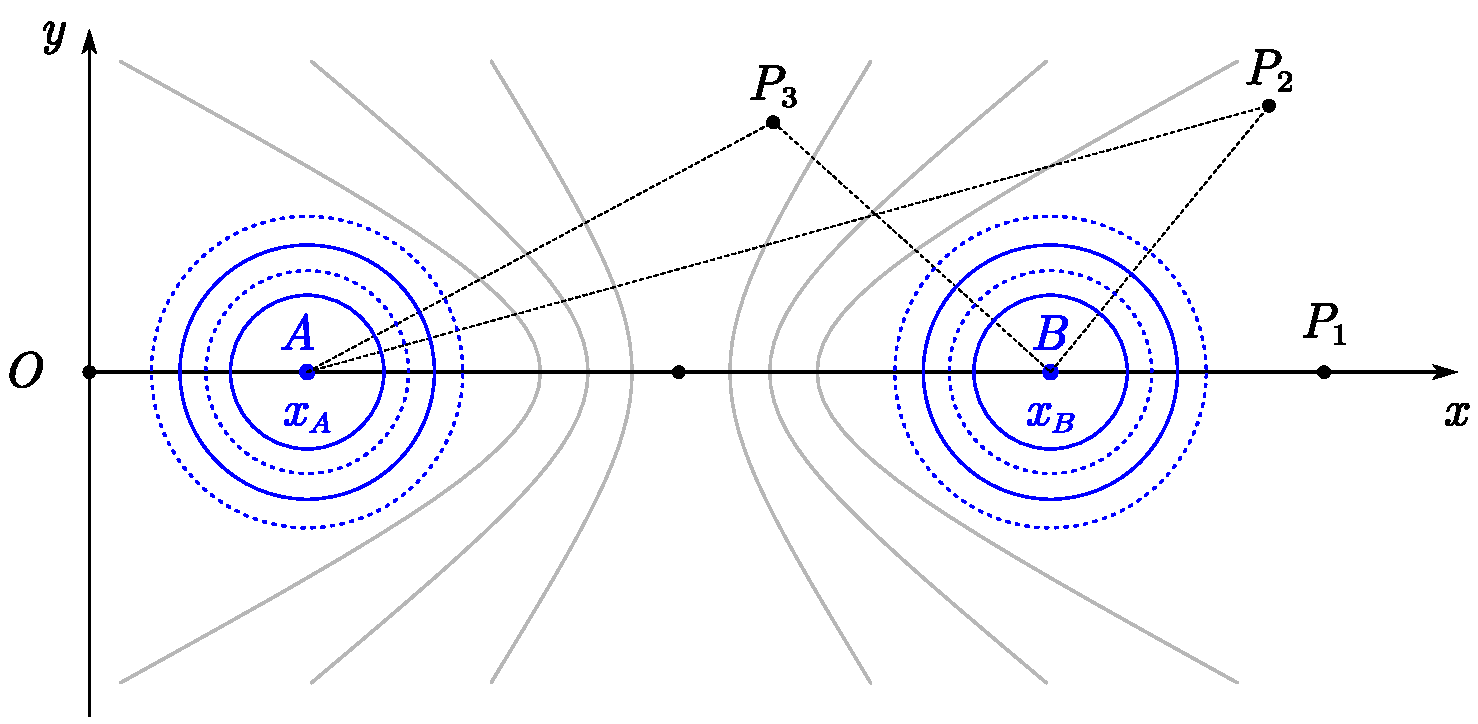
\includegraphics[height=120pt]{assets/3/crop_pdf_66eff444a80a6_f690229642a2b8bc66e9fbb05793266b_66eff43590e16.pdf}
        \caption{\bfseries 两球面波源或两柱面波源 }
    \end{subfigure}\hfill
    \begin{subfigure}[t]{0.49\columnwidth}\centering
        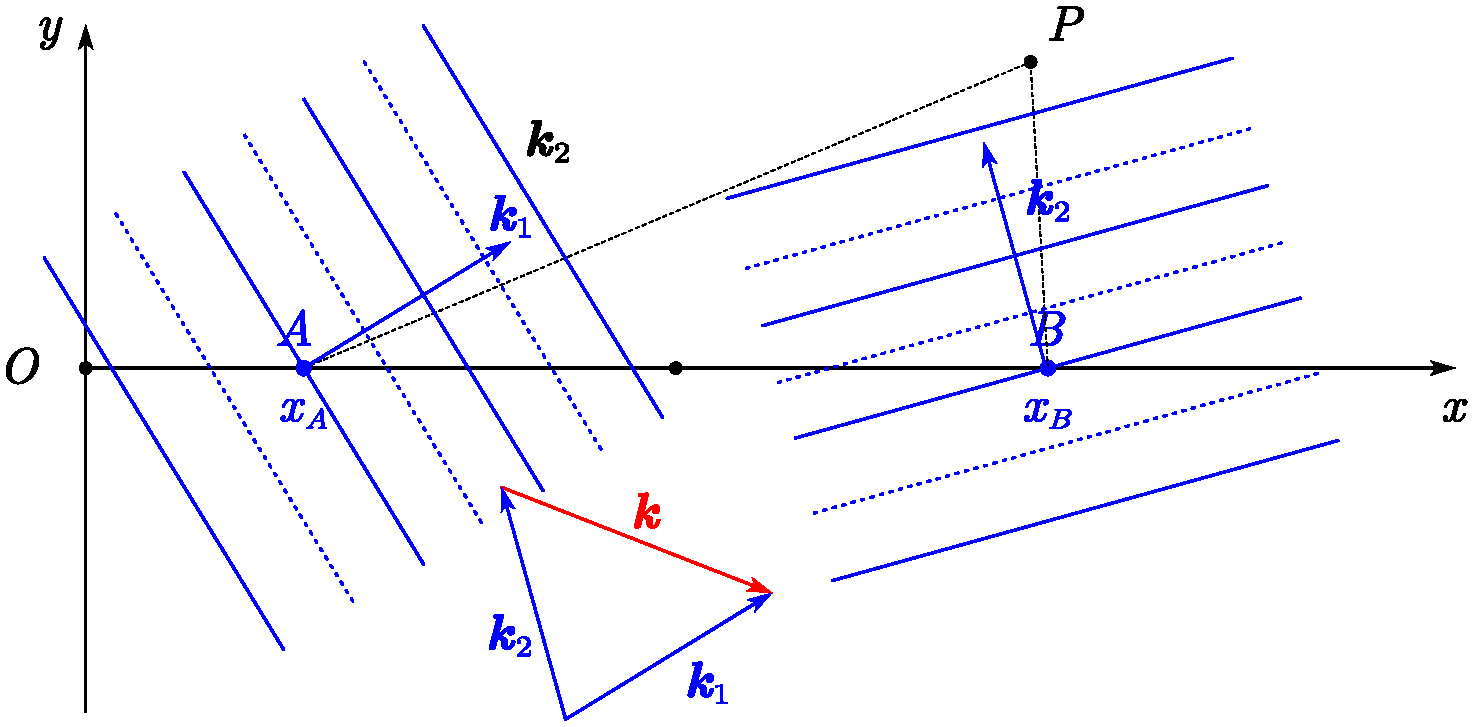
\includegraphics[height=120pt]{assets/3/双平面波源.pdf}
        \caption{\bfseries 两平面波源 }
    \end{subfigure}
    \caption{\bfseries 两个同频波源的干涉 }\label{两个同频波源的干涉}
\end{figure}


方便起见,不妨令 $\varepsilon_A = \varepsilon_B$,则合扰动为:
\begin{gather}
E = E_0 \cos \left(-\omega t + \alpha \right) = E_0 \cdot e^{i(-\omega t + \alpha)},\quad E_0 = \sqrt{\frac{A^2}{r_1^2} + \frac{B^2}{r_2^2} + \frac{2AB}{r_1r_2}\cos\left( k \left( r_1  - r_2 \right)\right)} \\ 
\sin \alpha = \frac{1}{E_0} \left( \frac{A}{ r_1 }\sin \alpha_A + \frac{B}{ r_2 } \sin \alpha_B\right),\quad \cos \alpha = \frac{1}{E_0} \left( \frac{A}{ r_1 }\cos \alpha_A + \frac{B}{ r_2 } \cos \alpha_B\right)\\ 
\alpha = 
\begin{cases}
    \arcsin \left[ \frac{1}{E_0} \left( \frac{A}{ r_1 }\sin \alpha_A + \frac{B}{ r_2 } \sin \alpha_B\right) \right] &, \cos \alpha \geqslant 0 \\
    \pi - \arcsin \left[ \frac{1}{E_0} \left( \frac{A}{ r_1 }\sin \alpha_A + \frac{B}{ r_2 } \sin \alpha_B\right) \right] &,  \cos \alpha < 0
\end{cases}
\end{gather}


对于可见光,其波长在 nm 级别,空间频率 $k = \frac{2\pi}{\lambda}$ 极高。为方便可视化,我们取波长 $\lambda = 0.4 \pi \ \mathrm{m}$,即 $k = 5$ 的微波,并令振幅系数 $A = 50$,$B = 50$,作出图像。图 \ref{单个球面波源在平面上的振荡情况} 展示了单个波源在平面上的振荡情况($t = 0$)。对两波源的干涉\footnote{源码见附录 \ref{单个球面波源在平面上的振荡情况 源码}},我们令两波源位置分别为 $(-2, 0)$,$(2, 0)$,作出图像,图 \ref{两个球面波源在平面上的干涉情况} 展示了它们的干涉情况($t = 0$)\footnote{源码见附录 \ref{两个球面波源在平面上的干涉情况 源码}}。单波源和双波源随时间的振动详见 GIF 动图 \href{https://www.123pan.com/s/0y0pTd-QwKj3}{(here)}。

\begin{figure}[H]\centering
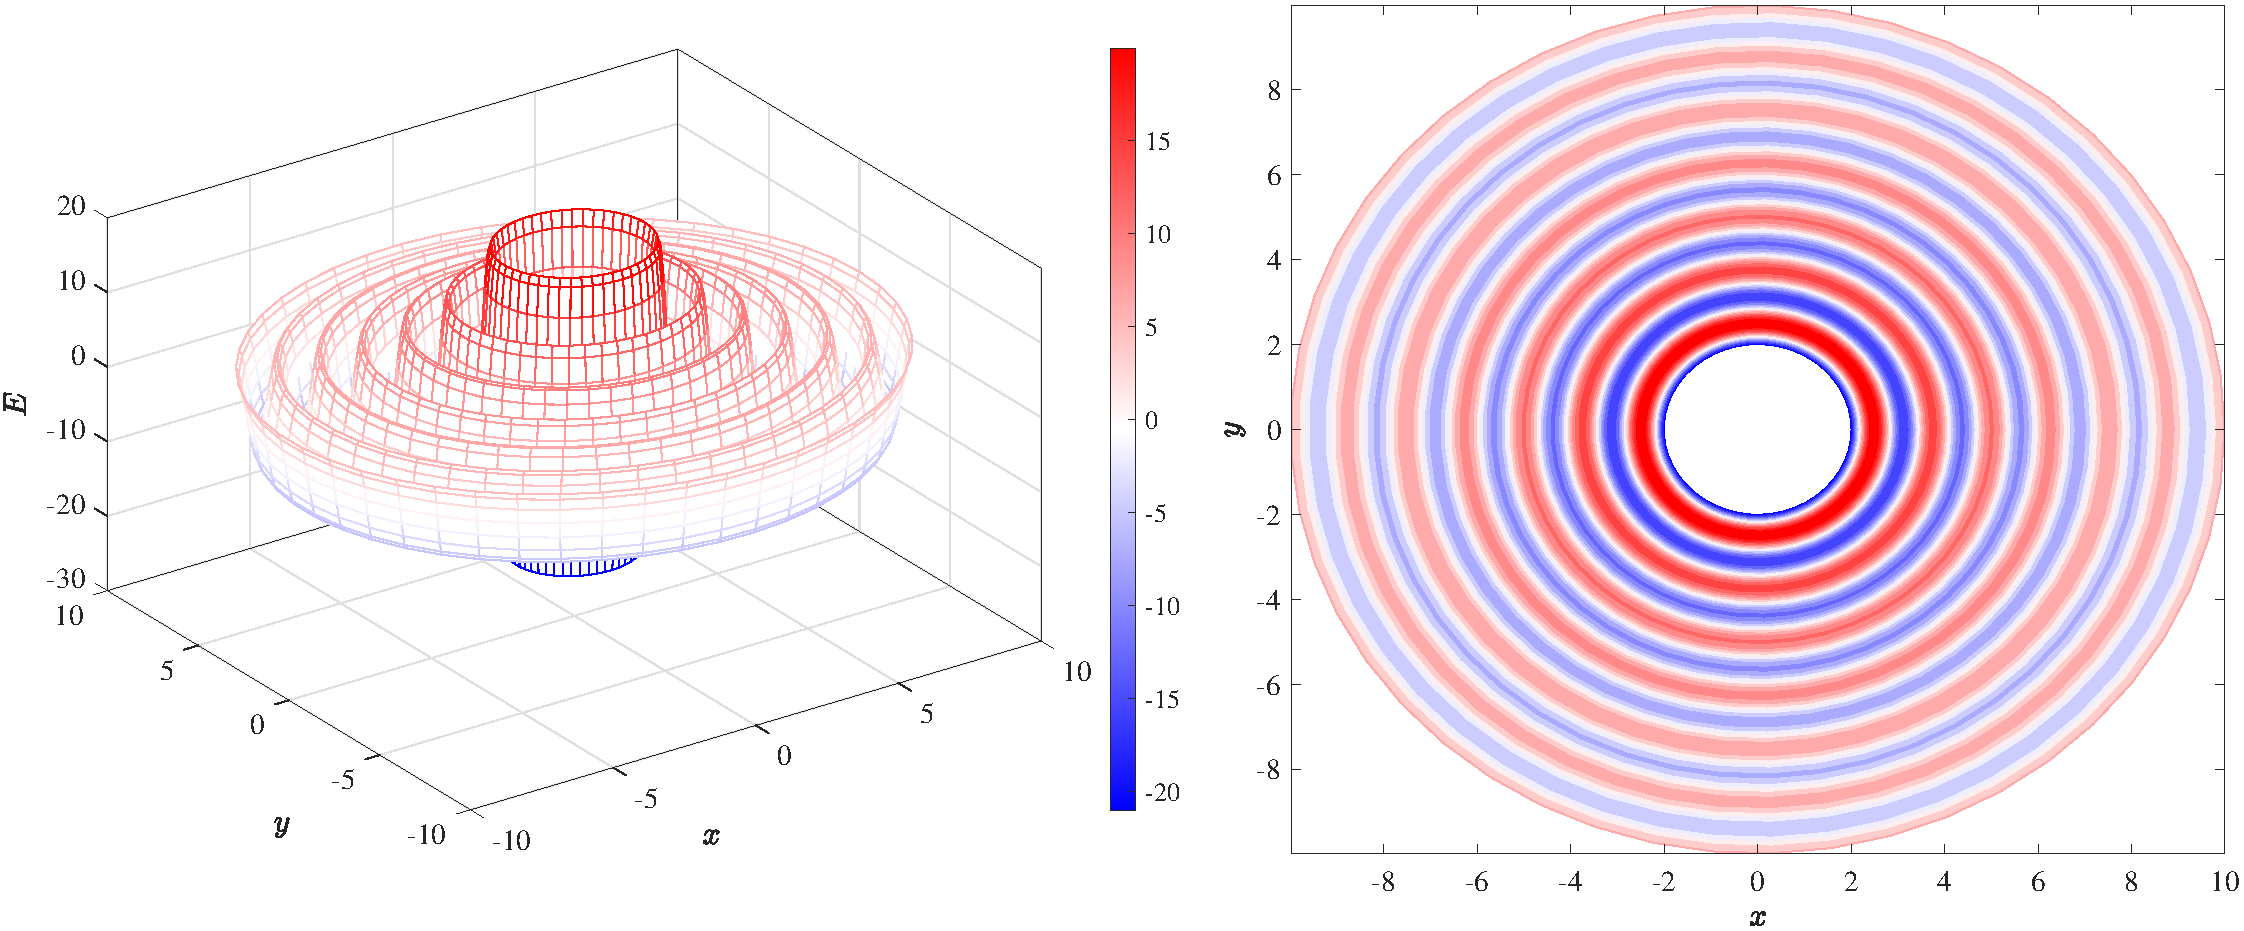
\includegraphics[width=0.95\columnwidth]{assets/3/单个球面波源.pdf}
\caption{\bfseries 单个球面波源在平面上的振荡情况}\label{单个球面波源在平面上的振荡情况}
\end{figure}

\begin{figure}[H]\centering
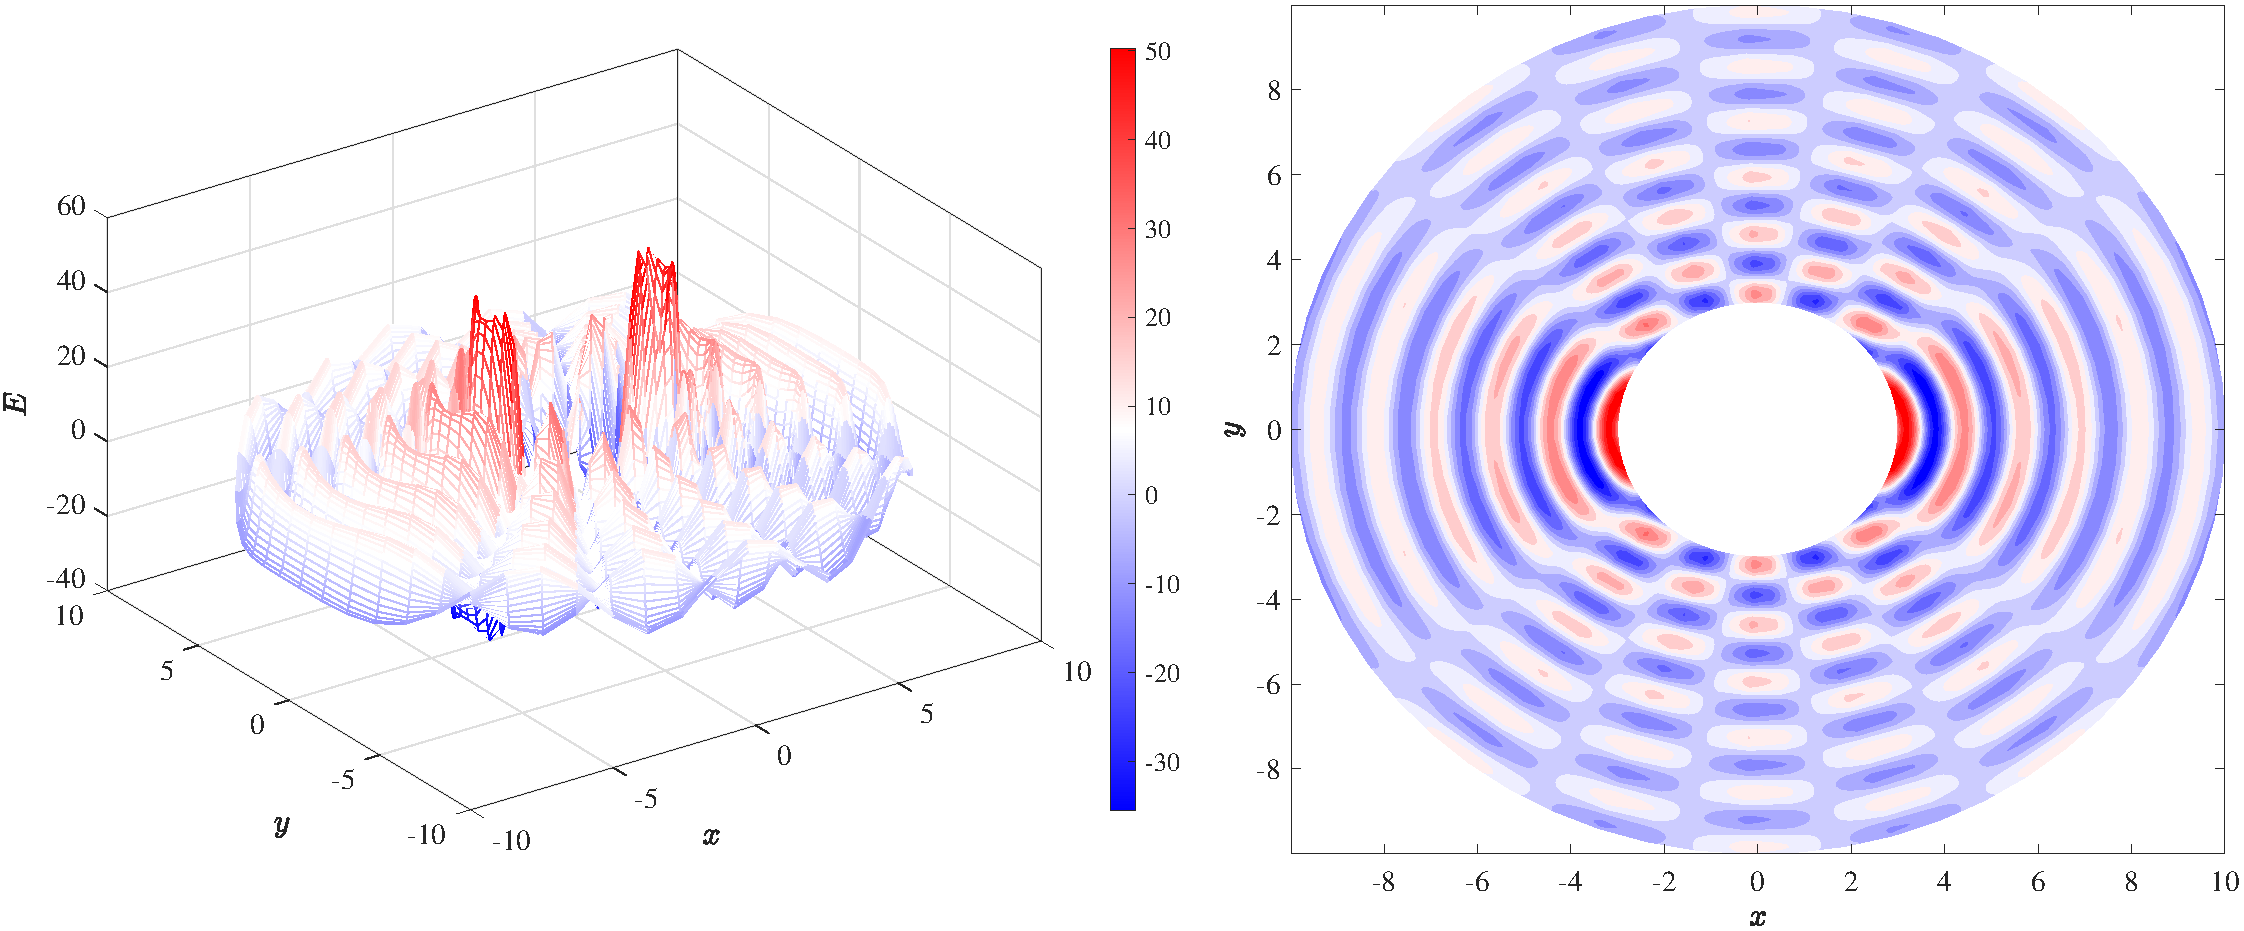
\includegraphics[width=0.95\columnwidth]{assets/3/两个球面波源.pdf}
\caption{\bfseries 两个球面波源在平面上的干涉情况}\label{两个球面波源在平面上的干涉情况}
\end{figure}

当点 $P$ 离波源极远时,近似有 $\frac{r_1}{r_2} = 1$(这与近似有 $r_1 - r_2 = 0$ 不同),将距离记为 $r$,则振幅的位置分布为 $E_0 = \frac{1}{r} \sqrt{ A^2 + B^2 + 2AB \cos (k(r_1 - r_2))} $。若可以认为 $\frac{1}{r}$ 近似不变,则此时,具有相同振幅大小的点,等价于 $\cos (k(r_1 - r_2))$ 具有相同的值,也即:
\begin{equation}
    | r_1 -  r_2| =  \frac{1}{k} (\theta + 2\pi n),\quad \theta \in [0, 2\pi),\  n = 0,1,2,\cdots
\end{equation}

对每个给定的 $n$,上述方程表示一条双曲线(焦点为两波源),因此上述方程构成一个双曲线族(空间中构成旋转双曲面族),如图 \ref{两个同频波源的干涉} (a) 中的灰色曲线所示。特别地,令 $\theta = 0$ 可以得到最大振幅对应的双曲线族,令 $\theta = \pi$,得到最小振幅对应的双曲线族。

由于球面波的旋转对称性,只需绕 $x$ 轴旋转一圈,即可得到整个空间上的振幅分布情况,也即两波源干涉情况。振幅的位置分布是较为重要的内容,在后文的干涉实验部分,我们将再次讨论这个问题。


\subsubsection{示例二:两柱面波}

考虑两柱面波的干涉情况,其中柱体的高与 $x$-$y$ 平面垂直。容易发现,这与球面波在 $x$-$y$ 平面的行为是相同的,仅需修改波源的振幅衰减系数。同样地,不妨令初相位 $\varepsilon_1 = \varepsilon_2$,得到合扰动:

\begin{gather}
    E = E_0 \cos \left(-\omega t + \alpha \right) = E_0 \cdot e^{i(-\omega t + \alpha)},\quad E_0 = \sqrt{\frac{A^2}{r_1} + \frac{B^2}{r_2} + \frac{2AB}{\sqrt{r_1r_2} }\cos\left( k \left( r_1  - r_2 \right)\right)} \\ 
    \sin \alpha = \frac{1}{E_0} \left( \frac{A}{ \sqrt{r_1} }\sin \alpha_A + \frac{B}{ \sqrt{r_2} } \sin \alpha_B\right),\quad \cos \alpha = \frac{1}{E_0} \left( \frac{A}{ \sqrt{r_1} }\cos \alpha_A + \frac{B}{ \sqrt{r_2} } \cos \alpha_B\right)\\ 
    \alpha = 
    \begin{cases}
        \arcsin \left[ \frac{1}{E_0} \left( \frac{A}{ \sqrt{r_1} }\sin \alpha_A + \frac{B}{ \sqrt{r_2} } \sin \alpha_B\right) \right] &, \cos \alpha \geqslant 0 \\
        \pi - \arcsin \left[ \frac{1}{E_0} \left( \frac{A}{ \sqrt{r_1} }\sin \alpha_A + \frac{B}{ \sqrt{r_2} } \sin \alpha_B\right) \right] &,  \cos \alpha < 0
    \end{cases}
\end{gather}
由于柱面波的平移对称性,只需沿 $z$ 轴进行平移,即可得到整个空间上的干涉情况。在平面内的其它性质与球面波类似。

\subsubsection{示例三:两平面波}

考虑两平面波的干涉情况,如图 \ref{两个同频波源的干涉} (b),平面波函数为:
\begin{gather}
    E_A = E_{A,0}\cdot e^{i(-\omega t + k r_1 + \varepsilon_A)},\quad \ \alpha_A = \boldsymbol{k_1}  \cdot  \boldsymbol{x}_{AP} + \varepsilon_A
    \\
    E_B = E_{B,0} \cdot e^{i(-\omega t + k r_2  + \varepsilon_B)}\quad  \alpha_B = \boldsymbol{k_2} \cdot \boldsymbol{x}_{BP}  + \varepsilon_B
\end{gather}
令 $\varepsilon_1 = \varepsilon_2$,得到合扰动:
\begin{gather}
    E = E_0 \cos \left(-\omega t + \alpha \right) = E_0 \cdot e^{i(-\omega t + \alpha)} \\ 
    E_0 = \sqrt{E_{A,0}^2 + E_{B,0}^2 + 2 \cos \left( \Delta \alpha \right)} ,\quad \Delta \alpha =  (\boldsymbol{k_1} -\boldsymbol{k_2})\cdot \boldsymbol{x} + (\boldsymbol{k_2}\cdot \boldsymbol{x}_B - \boldsymbol{k_1} \cdot \boldsymbol{x}_A)\\ 
        \sin \alpha = \frac{1}{E_0}\left[ E_{A,0}\sin ( \boldsymbol{k_1}  \cdot  \boldsymbol{x}_{AP}) + E_{B,0}\sin (\boldsymbol{k_2} \cdot \boldsymbol{x}_{BP}) \right] \\ 
        \cos \alpha = \frac{1}{E_0}\left[ E_{A,0}\cos ( \boldsymbol{k_1}  \cdot  \boldsymbol{x}_{AP}) + E_{B,0}\cos (\boldsymbol{k_2} \cdot \boldsymbol{x}_{BP}) \right] \\ 
    \alpha = 
    \begin{cases}
        \arcsin \left[ \frac{1}{E_0}\left( E_{A,0}\sin \alpha_A + E_{B,0}\sin \alpha_B \right)  \right] &, \cos \alpha \geqslant 0 \\
        \pi - \arcsin \left[ \frac{1}{E_0}\left( E_{A,0}\sin \alpha_A + E_{B,0}\sin \alpha_B \right)  \right] &,  \cos \alpha < 0
    \end{cases}
\end{gather}

由于 $\boldsymbol{k_1} \cdot \boldsymbol{x}_A$ 和 $\boldsymbol{k_2} \cdot \boldsymbol{x}_B$ 是定值,而 $\boldsymbol{k} = \boldsymbol{k_1} - \boldsymbol{k_2}$ 构成一个新的传播矢量,因此合成后的波仍是平面波(但不均匀,振幅是位置的函数),或者说每个等相面仍构成一个平面。

类似地,由平面波的平移对称性,沿 $z$ 轴平移即可得全空间的合成情况。

\subsection{多个同频波源的干涉}

上面的结论容易推广到任意 $n$ 个扰动叠加,即:
\begin{gather}
    E = E_0 \cos \left(-\omega t + \alpha \right) = E_0 \cdot e^{i(-\omega t + \alpha)}
    \\ 
    E_0 = \sqrt{\left( \sum_{i=1}^n E_{i,0}\sin \alpha_i \right)^2 + \left( \sum_{i=1}^n E_{i,0}\cos \alpha_i \right)^2 }   \\ 
    =  \sqrt{\sum_{i=1}^n E_{i,0}^2 + \sum_{1 <= i < j <= n} 2E_{i,0}E_{j,0}\cos(\alpha_i - \alpha_j)},\quad
    \\ 
    \sin \alpha = \frac{1}{E_0}\sum_{i=1}^n E_{i,0}\sin \alpha_i ,\quad 
    \cos \alpha = \frac{1}{E_0}\sum_{i=1}^n E_{i,0}\cos \alpha_i \\ 
    \alpha = 
    \begin{cases}
        \arcsin \left( \frac{1}{E_0}\sum_{i=1}^n E_{i,0}\sin \alpha_i  \right) &, \cos \alpha \geqslant 0 \\
        \pi - \arcsin \left( \frac{1}{E_0}\sum_{i=1}^n E_{i,0}\cos \alpha_i  \right) &,  \cos \alpha < 0
    \end{cases} \\ 
    I = \sum_{i=1}^n I_i + \sum_{1 <= i < j <= n} 2\sqrt{I_iI_j} \cos(\alpha_i - \alpha_j) 
\end{gather}

\section{不同频率光的干涉}

\section{产生干涉的实际条件}

前面我们已经提到,在叠加(或干涉)问题中,电场的振幅通常只是位置的函数,而与时间无关,其实这也是观察到干涉图样的必要条件。观察干涉图样,无非是用照片(视频等同于照片)、人眼、辐射计以及类似的传感器,它们都有一定的“曝光时间”,我们只能观察到在曝光时间内,光强或辐射强度的平均值,即:

\begin{equation}
I = I_1 + I_2 + 2 \sqrt{I_1 I_2} \frac{1}{\tau} \int_{0}^{\tau}  \cos(\Delta \alpha) \mathrm{d} t
\end{equation}
其中 $\tau$ 为仪器的曝光时间。对可见光而言,其振荡周期 $T = \frac{\lambda}{v}$ 在 $10^{-15}$ s 级别,因此 $\tau$ 通常远大于 $T$,这样,我们只能观察到平均光强,而无法观察到光强的瞬时变化。如果 $\Delta \alpha$ 与时间无关,或者在曝光时间内几乎保持不变,那么就能得到(观察到)稳定的干涉图样。否则恒有 $I = I_1 + I_2$,是平凡的叠加,观察不到干涉现象。

另外,若两波源的振动方向垂直,电场也仅是平凡的叠加,而不会产生干涉。因此,干涉现象要求两波源振动方向不能垂直。

还有一种情况是,实际中的波源(光源)大多不能产生理想的、初相位不变的单频波。

例如,对普通光源(如白炽灯),光是由光源中的原子、分子发生能级跃迁时发出的,跃迁时发出的波列都是有限长的,且初相位随机,持续时间通常短于 10 ns,在此时段内,光场振荡约百万次。对于外界的探测设备来讲,10 ns 仍是一个极短的时间,通常远远小于曝光时间。因此,即使每个波列的初相位都相同,在曝光时间内的上万个波列的平均下,积分项 $\int_{0}^{\tau}  \cos(\Delta \alpha) \mathrm{d} t$ 为 0,$I = I_1 + I_2$,导致观察到的强度分布仅为平凡的叠加,无法观察到干涉。

上面光源发出的光的初相位是时间的函数,随着时间快速变化,无法产生干涉,称其为不相干光源。在实际中,还有一些光源,并不能达到完美的点光源,而是有一定的光源宽度,当宽度较大时,不同位置上光的叠加,会导致条纹的对比度降低(甚至为 0),称为空间不相干。另外有一些光源,发出的光具有多个波长(或者频谱较均匀),不同波长相互叠加导致相干性降低,称为时间不相干。

%\includemedia[
%  width=10cm,
%  height=5cm,
%  activate=pageopen,
%  addresource=test.mp4,
%  flashvars={source=test.mp4}
%]{}{VPlayer.swf}

%\includemedia[
%  label=some_dice,
%  width=1.0\linewidth,height=0.675\linewidth, % 16:9
%  addresource=test.mp4, 
%  transparent,
%  activate=pageopen,
%  passcontext,
%  flashvars={
%    source=test.mp4
%   &autoPlay=true % start playing on activation
%   &loop=true
%  }
%]{}{VPlayer.swf}
%% loop video
%\mediabutton[
%  mediacommand=some_dice:playPause,
%  overface=\color{blue}{\fbox{\strut Play/Pause}},
%  downface=\color{red}{\fbox{\strut Play/Pause}}
%]{\fbox{\strut Play/Pause}}
%\mediabutton[
%  mediacommand=some_dice:setSource [(test.mp4)]
%]{\fbox{\strut Media Caption}}


\section{分波前干涉}

波前,即波面,也称波阵面或等相面。“分波前”干涉,是依据惠更斯原理,将一个波面分为两个(或多个)波面,最终产生干涉现象。

\subsection{杨氏双缝干涉实验}

杨氏双缝干涉装置如图 \ref{杨氏双缝干涉装置} (a),$S$ 为一狭缝,$S_1$ 和 $S_2$ 为一对狭缝,最右侧的屏为观察屏。由惠更斯原理,一平面波(可借助激光器和透镜产生)传播到狭缝 $S$ 时,以柱面波形式出射,在遇到双缝屏时,分化为两个柱面波继续前进,从而产生干涉,并在观察屏上显现出来。与杨氏实验原理类似的有洛埃德镜实验、菲涅尔双棱镜、菲涅尔双面镜等,它们的 GIF 动图见链接 \href{https://www.123pan.com/s/0y0pTd-5wKj3}{(here)}。

如果杨氏实验中双缝屏上的双缝对称分布,一般可认为分化的两个柱面波具有相同的初相位和振幅。装置中各参量的典型值是:
\begin{equation}
d = 100 \ \mathrm{\mu m},\  R = 5\ \mathrm{cm},\ D = 1\ \mathrm{m},\ L = 4 \ \mathrm{cm},\quad D \gg L \gg d
\end{equation}

设通过双缝屏后,两柱面波的振幅系数相同,都为 $A$,真空介电常量 $\varepsilon_0 = 8.854187817 \times 10^{-12}\ \mathrm{F\cdot m^{-1}}$,真空磁导率 $\mu_0 = 4\pi \times 10^{-7}\ \mathrm{N\cdot A^{-2}}$,则两波的光强度分别为
\begin{equation}
    I_1 = \frac{1}{2}\sqrt{\frac{\varepsilon_0}{\mu_0}}E_{1,0}^2 = \frac{1}{2}\sqrt{\frac{\varepsilon_0}{\mu_0}} \cdot \frac{A^2}{r_1},\quad
    I_2 = \frac{1}{2}\sqrt{\frac{\varepsilon_0}{\mu_0}} \cdot \frac{A^2}{r_2}
\end{equation}
那么,接受屏上的振幅和强度分布为:
\begin{equation}
    E_0 = A \sqrt{ \frac{1}{r_1} + \frac{1}{r_2} + \frac{2}{\sqrt{r_1r_2}} \cos \left( \frac{2 \pi}{\lambda}(r_1 - r_2) \right)  }  ,\quad 
    I = A^2\sqrt{\frac{\varepsilon_0}{\mu_0}}\left[ \frac{1}{2}\left( \frac{1}{r_1} + \frac{1}{r_2} \right) + \frac{\cos \left( \frac{2 \pi}{\lambda}(r_1 - r_2) \right)}{\sqrt{r_1r_2} } \right]
\end{equation}
装置参数在典型值附近时,可以有近似:
\begin{equation}\label{杨氏双缝干涉近似}
\frac{r_1}{D} = \frac{r_2}{D} = 1,\quad r_2 - r_1 = \frac{d}{\sin \theta} = \frac{d}{\sin \theta} = \frac{x d}{ D },\quad I_1 = I_2
\end{equation}
得到近似后的振幅和强度分布如下,其中 $\Delta x= \frac{\lambda D}{b}$ 称为条纹间距。
\begin{gather}\label{杨氏双缝干涉近似结果}
    E_0(x) = \frac{\sqrt{2}A}{\sqrt{D}} \cdot \sqrt{1 + \cos \left( \frac{2 \pi d}{\lambda D}x \right)} = \frac{\sqrt{2}A}{\sqrt{D}} \cdot \sqrt{1 + \cos \left( \frac{2 \pi x}{\Delta x} \right)} \\ 
    I(x) = \sqrt{\frac{\varepsilon_0}{\mu_0}} \cdot \frac{A^2}{D} \left[ 1 + \cos \left( \frac{2 \pi  d}{\lambda D }x \right) \right] = \sqrt{\frac{\varepsilon_0}{\mu_0}} \cdot \frac{A^2}{D} \left[ 1 + \cos \left( \frac{2 \pi x}{\Delta x} \right) \right]
\end{gather}

\begin{figure}[H]\centering
    \begin{subfigure}[t]{0.52\columnwidth}\centering
        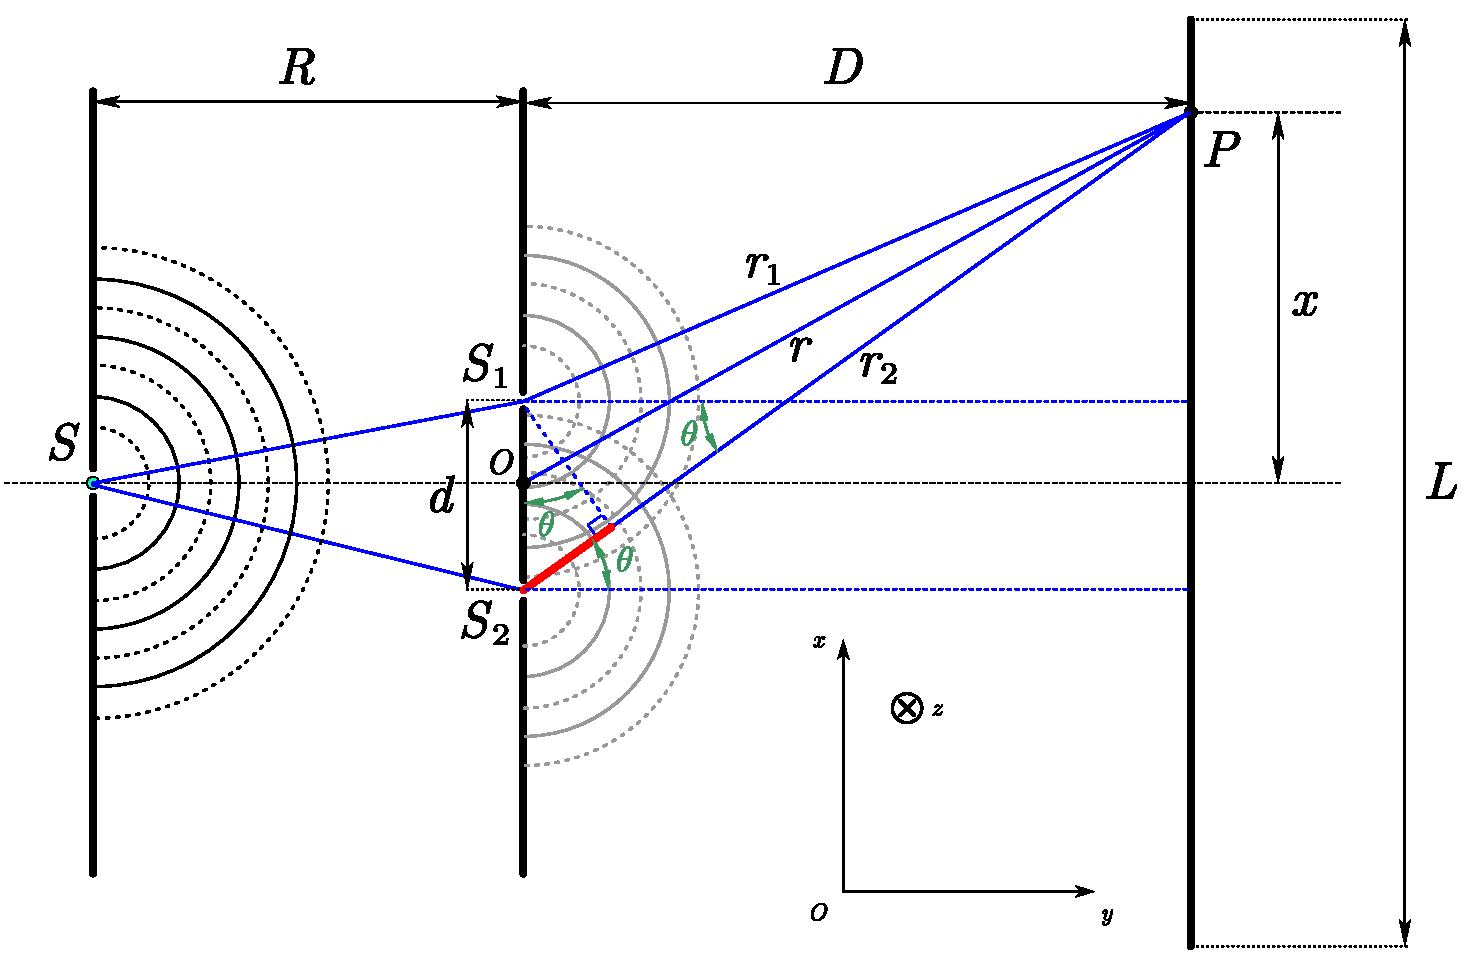
\includegraphics[height=165pt]{assets/3/杨双.pdf}
        \caption{\bfseries 杨氏双缝干涉装置 }
    \end{subfigure}\begin{subfigure}[t]{0.48\columnwidth}\centering
        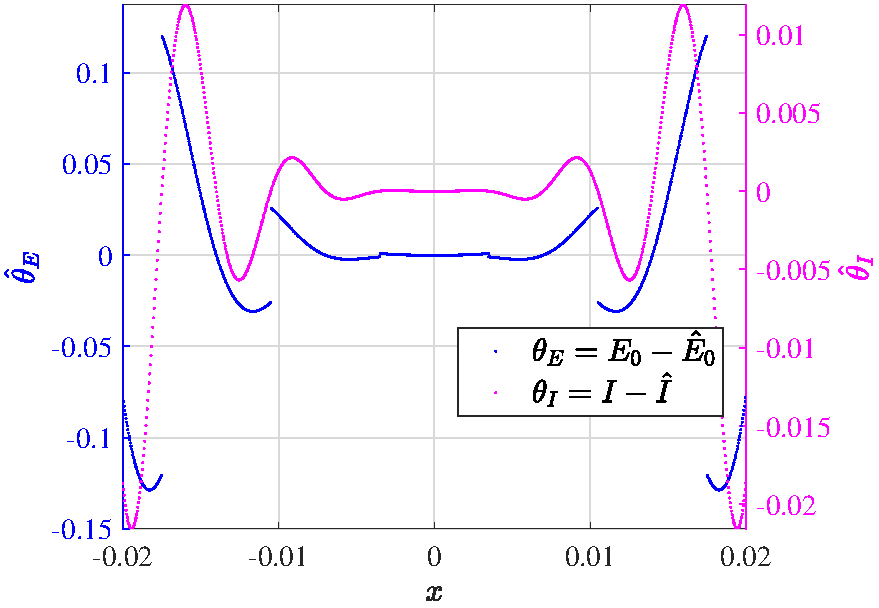
\includegraphics[height=165pt]{assets/3/杨残差.pdf}
        \caption{\bfseries 近似模型残差分布 }
    \end{subfigure}
    \caption{\bfseries 杨氏双缝干涉装置与近似模型残差分布 }\label{杨氏双缝干涉装置}
\end{figure}

图 \ref{近似模型与非近似模型的比较} 展示了未近似和近似时,振幅、光强在接受屏上的分布情况,图 \ref{杨氏双缝干涉装置} (b) 是近似与未近似模型的残差分布\footnote{图 \ref{杨氏双缝干涉装置} (b) 与图 \ref{近似模型与非近似模型的比较} 源码见附录 \ref{杨氏双缝干涉装置 源码}},其中装置参数采取典型值。计算得到一些误差参数(对横坐标均匀离散 1000 个点)如下\footnote{这些误差参数的定义见附录 \ref{} 或网址 (here)}: 
\begin{gather}
\begin{matrix}
    \text{相对平均值误差:} \text{RME}_{E_0} =  0.0001336621,\quad \text{RME}_{I} = 0.0002192205 \\
    \text{决定系数:} \text{R}^2_{E_0} =  0.9999969495,\quad \text{R}^2_{I} = 0.9999975710 \\
    \text{调整决定系数:} \text{R}^2_{\text{adj}, E_0} = 0.9999969464,\quad \text{R}^2_{\text{adj}, I} = 0.9999975686 \\
    \text{平均标准绝对残差:} \text{RS}_{E_0} = 0.0005191648,\quad \text{RS}_{I} = 0.0006515739\\
    \text{平均标准平方残差:} \text{RSS}_{E_0} = 0.0000007426 ,\quad \text{RSS}_{I} = 0.0000012850  \\ 
    \text{标准面积误差:} \text{SAE}_{E_0} = 0.0005185186 ,\quad \text{SAE}_{I} = 0.0006493885
\end{matrix}
\end{gather}


由图 \ref{杨氏双缝干涉装置} (b),图 \ref{近似模型与非近似模型的比较} 和几个误差参数可以看到,近似效果较好。

\begin{figure}[H]\centering
\begin{subfigure}[t]{0.5\columnwidth}\centering
    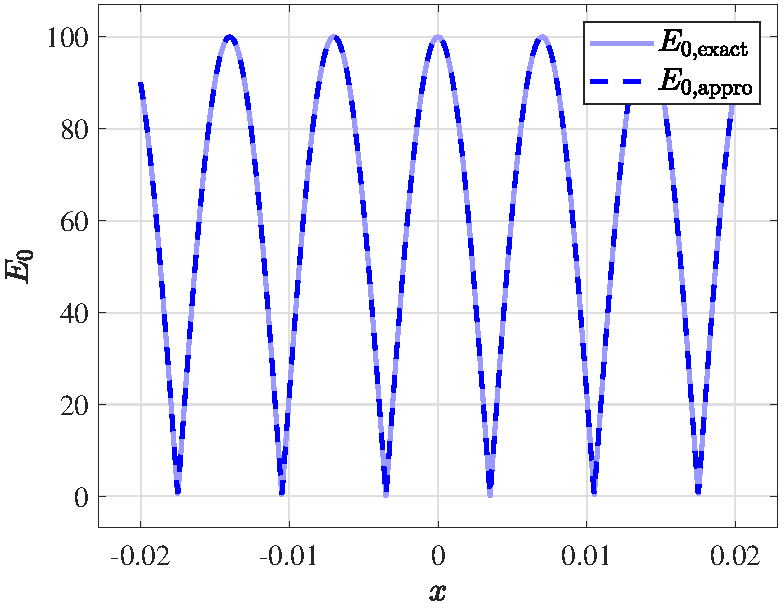
\includegraphics[height=165pt]{assets/3/杨电场.pdf}
    \caption{\bfseries 电场振幅位置分布 }
\end{subfigure}\hfill
\begin{subfigure}[t]{0.5\columnwidth}\centering
    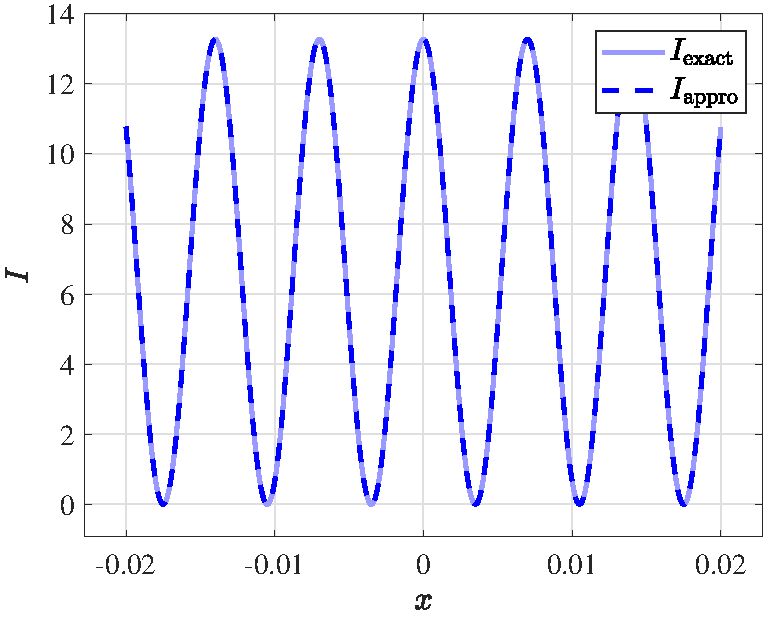
\includegraphics[height=165pt]{assets/3/杨光强.pdf}
    \caption{\bfseries 光强位置分布 }
\end{subfigure}
\caption{\bfseries 近似模型与非近似模型的比较 }\label{近似模型与非近似模型的比较}
\end{figure}

\noindent 杨氏双缝干涉的特点:
\begin{enumerate}
\item 非定域干涉:在干涉场中离双孔不太近也不太远的区域处处有干涉
\item 自相干:相干光波来自同一波源
\item 定态干涉:振幅(或强度)在干涉场中的分布仅与位置有关,与时间无关
\end{enumerate}


白光光源与其他补充内容详见 \href{https://produckthieves.home.blog/2020/02/10/phy-c15-double-slit-interference/}{PHY C15: Double Slit Interference}、\href{https://www.physics.louisville.edu/cldavis/phys299/notes/lo_interference.html}{University of Louisville: Double Slit Interference} 以及 \href{https://zhuanlan.zhihu.com/p/335815195}{知乎:双缝干涉实验}。我们不多赘述。

\subsection{杨氏实验中干涉条纹的移动}

为提高分析效率,此节的推导都采用近似模型。接受屏上相邻明(暗)条纹的间距 $\Delta x$ 为:
\begin{equation}
\Delta x = \frac{D \lambda}{d}
\end{equation}
取 $\lambda = 700.0\ \mathrm{nm}$ 的红光,$\Delta x = 7 \ \mathrm{mm}$,可被人眼分辨。称 $\frac{\Delta x}{2}$ 为条纹宽度,此时条纹宽度为 $3.5\ \mathrm{mm}$。

下面依次讨论光源位置、光源宽度对干涉条纹的影响。先考虑理想点光源的微小移动引起的干涉条纹移动。当点光源位于中轴线上时,0 级明纹也在轴上,假设光源 S 向下移动距离 $| \delta_s |$,也即向上移动 $(-\delta_s)$,在近似条件 \ref{杨氏双缝干涉近似} 下,以及 $R \gg d$ 时近似有 $R_1 - R_2 = \frac{d(-\delta_s)}{R}$,得到 0 级明纹向上移动的距离 $\delta_x$: 
\begin{equation}
\delta_x = - \frac{D}{R}\delta_s
\end{equation}
负号表示两者移动方向相反。

实际光源并非是理想的点光源,而是有一定的光源宽度,虽然对干涉条纹位置影响不大,但会对条纹对比度产生明显的影响。理想点光源不在中央时,屏幕上的强度分布大小可以近似不变,仅是发生上下平移。记点光源位置为 $\delta_s$,在公式 \ref{杨氏双缝干涉近似结果} 中作映射 $x \longrightarrow x - \delta_x$,并简记接受屏上的最大光强为 $I_{\text{max}} = 2 \frac{\varepsilon_0}{\mu_0} \cdot \frac{A^2}{r}$,简记 $x$ 前的系数为 $\eta = \frac{2 \pi}{\Delta x}$,得到新的强度分布:
\begin{align}
I(x) &= \frac{I_{\text{max}}}{2}\left[
1 + \cos \left( \eta (x - \delta_x)\right)
\right] = \frac{I_{\text{max}}}{2}\left[
    1 + \cos \left( \eta x + \eta\frac{D}{R}\delta_s\right)
    \right]
\\
= &
\frac{I_{\text{max}}}{2}\left[
1 + \cos \left( \eta x \right)\cos \left(\eta\frac{D}{R}\delta_s \right) - \sin \left( \eta x \right)\sin \left( \eta\frac{D}{R}\delta_s \right)
\right],\quad \eta = \frac{2 \pi}{\Delta x}
\end{align}



设光源在中央且宽度为 $b$(即发光区域在 $[-\frac{2}{b},\ \frac{2}{b}]$),光源均匀发光(事实上这个条件比较苛刻,现实中的激光器无法做到,需要对光线进行处理),屏幕上的强度分布 $I(x, b)$ 为:
\begin{gather}
I(x, b) = \frac{I_{\text{max}}}{2b} \int_{-\frac{b}{2}}^{\frac{b}{2}} \left[ 1 + \cos \left( \eta x \right)\cos \left( \eta\frac{D}{R}\delta_s \right) - \sin \left( \eta x \right)\sin \left( \eta\frac{D}{R}\delta_s \right) \right] \mathrm{d} \delta_s \\ 
= \frac{I_{\text{max}}}{2} \left[ 1 + \frac{\sin \left( \frac{\eta D}{2 R} b \right)}{\frac{\eta D}{2 R} b}\cdot \cos \left( \eta x \right) \right] = \frac{I_{\text{max}}}{2} \left[ 1 + \frac{\sin \left( \frac{\pi d}{\lambda R} b \right)}{\frac{\pi d}{\lambda R} b}\cdot \cos \left( \frac{2 \pi x}{\Delta x}  \right) \right]
\end{gather}

对任意给定的光源宽度 $b$,光强的最大最小值为 $1 \pm \left|  \frac{\sin u}{u} \right|$ ,其中 $u = \frac{\pi d}{\lambda R} b$,于是干涉条纹对比度 $\gamma$:
\begin{equation}
    \gamma = \gamma(b) = \left| \frac{\sin u}{u} \right| = \left| \frac{\sin \left( \frac{\pi d}{\lambda R} b \right)}{\frac{\pi d}{\lambda R} b} \right|
\end{equation}

强度分布 $I(x, b)$ 与干涉条纹对比度 $\gamma(b)$ 如图 \ref{光源宽度} 所示\footnote{源码见附录 \ref{光源宽度 源码}},当 $b = \frac{\lambda R}{d}$ 时,对比度为 0,完全看不到干涉条纹,将其称为光源极限宽度,此时认为光源完全不相干。

\begin{figure}[H]\centering
\begin{subfigure}[t]{0.5\columnwidth}\centering
    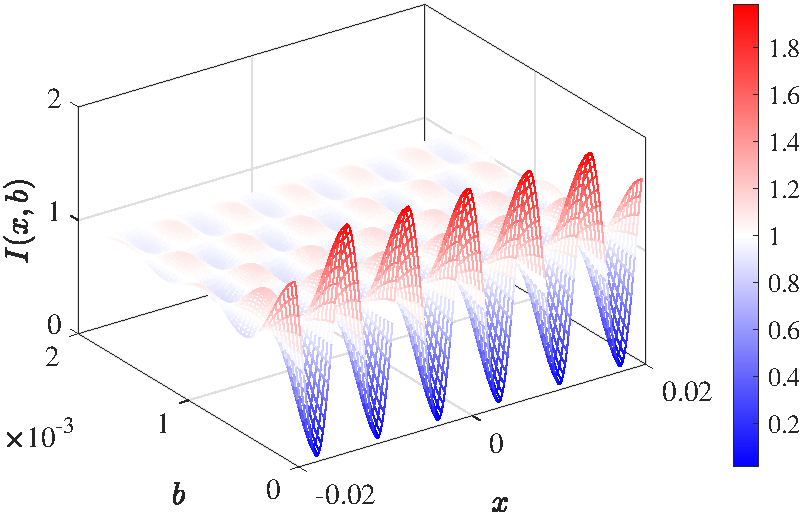
\includegraphics[height=160pt]{assets/3/光强分布.pdf}
    \caption{\bfseries 光强分布随光源宽度的变化 }
\end{subfigure}\hfill
\begin{subfigure}[t]{0.5\columnwidth}\centering
    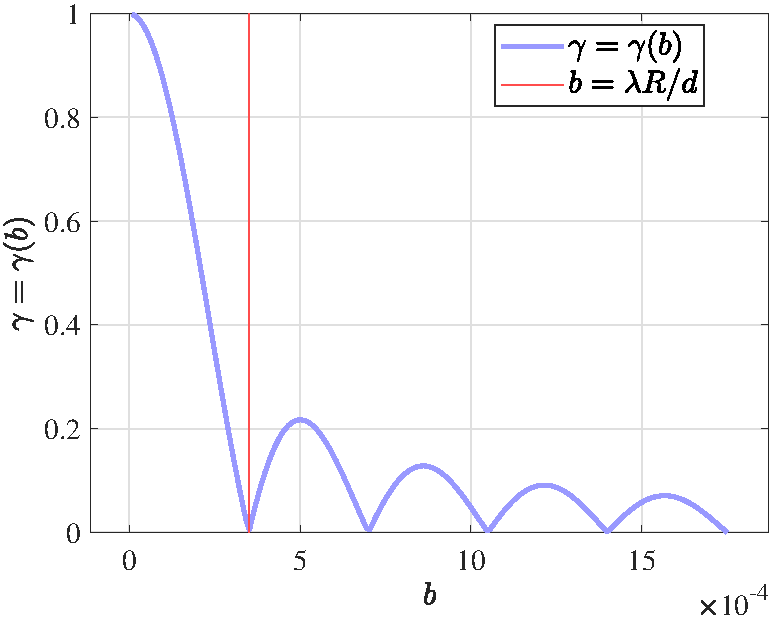
\includegraphics[height=160pt]{assets/3/干涉条纹对比度.pdf}
    \caption{\bfseries 干涉条纹对比度随光源宽度的变化 }
\end{subfigure}
\caption{\bfseries 光源宽度对干涉条纹的影响 }\label{光源宽度}
\end{figure}

\section{分振幅干涉}

https://zhuanlan.zhihu.com/p/145785676 薄膜干涉

光路可逆性推导振幅系数相同



\section{等倾干涉与等厚干涉}
\section{迈克尔逊干涉与}
\section{光场的空间相干性与时间相干性}
\section{多光束干涉}
\section{激光}







































































































\nocite{*}
\bibliography{re}
\thispagestyle{fancy} 
\addcontentsline{toc}{chapter}{参考文献}





















% --------------------------- 附录 --------------------------- %
% >> ------------------------ 附录 ------------------------ << %


\newpage
\appendix
% chapter 标题自定义设置
\titleformat{\chapter}[hang]{\normalfont\huge\bfseries\centering}{}{20pt}{}
\titlespacing*{\chapter}{0pt}{-25pt}{8pt} % 控制上方空白的大小
% section 标题自定义设置 
\titleformat{\section}[hang]{\normalfont\centering\Large\bfseries}{\thesection}{8pt}{}

% 附录 A
\chapter*{附录 A\hspace*{20pt} 波理论}\addcontentsline{toc}{chapter}{附录 A\hspace*{6pt} 波理论}   
\thispagestyle{fancy} 
\setcounter{section}{0}   
\renewcommand\thesection{A.\arabic{section}}   
\renewcommand{\thefigure}{A.\arabic{figure}} 
\renewcommand{\thetable}{A.\arabic{table}}


光的真实本性是光学的全部讨论的中心问题, 在本书中我们从头到尾都得对待这个问题。“光究竟是一种波动现象还是一种粒子现象?” 这个似乎干脆利索的问题, 远比它初看之下复杂得多。

因为对光的经典讨论和量子力学讨论都要用到波的数学描述, 本章要为这两种表述所需
要的东西打好基础。下面叙说的想法将用于一切物理波, 从一杯茶的表面张力皱波, 到从某个遥远的星系照到我们的光脉冲。

\section{一维波}

\subsection{$n$ 维波的概念}

一维波指的是在一维空间中传播的波,或者可以看作在一维空间中传播的波。例如一束光在空间中传播,沿其传播方向建立 $x$ 轴,则有 $E = E_0 e^{kx - \omega t}$(具有正负),这束光便可视为一维波。

一维波函数的最一般的形式:
\begin{equation}
\psi(x,t) = f(x-vt) = g(kx - \omega t)
\end{equation}

具体而言,对于给定的波形(波的形状),我们只需令 $t=0$,拍一张“照片”(例如 $\psi(x) = \frac{3}{10x^2+1}$),得到 $\psi(x,0) = f(x)$,然后将 $f(x)$ 中的 $x$ 换为 $x-vt$,即可得到一个以速度 $v$(可为负) 向 $x$ 轴正方向运动的波 $\psi(x,t) = f(x - vt) = g(kx - \omega t)$。
{\par\color{gray}\small
绳索的上下振动是在第二个维度上的,但振动导出的波仍是一维波。
\par}


\subsection{波动方程}

线性、各向同性、无损耗介质中的波动方程(也称波动微分方程)为:
\begin{equation}
    \frac{\partial^{2}\psi}{\partial x^{2}}=\frac{1}{v^{2}}\frac{\partial^{2}\psi}{\partial t^{2}} 
\end{equation}

如果代表一个波的函数 $\psi$ 是这个方程的解, 它将同时是 $(x-vt)$ 的函数(即 $kx - \omega t$ 的函数),它还是一个可以同时对 $x$ 和 $t$ 以非平庸方式求二次微商的函数。特别地,我们有结论:$\psi$ 是一维波函数 $\Longleftrightarrow$ $\psi$ 是 $(x-vt)$ 的二次可微函数 $\Longleftrightarrow$ $\psi$ 是 $(kx - \omega t)$ 的二次可微函数。

\section{谐波}

\subsection{相位和相速度}
考虑任何一个一维波函数 $\psi(x,t) = A \cos(\phi(x,t)) = A \cos (kx - \omega t + \phi_0) $,其中 $\phi = kx+vt + \phi_0$ 称为相位,$\phi_0$ 称为初相(也常用 $\varepsilon$ 表示)。只要相位中的 $kx$ 与 $\omega t$ 符号相反,即 $(kx - \omega t)$ 或 $(\omega t - kx)$,则波沿 $x$ 轴正方向传播,否则沿 $x$ 轴负方向。


\subsection{谐波的概念} 
谐波,指简谐波、正弦波,其轮廓图是正弦曲线,是最简单的波形。在后续的傅里叶变换一节我们可以看到,任何波形都可以由谐波叠加合成,因此谐波具有特殊的意义。
考虑如下波形:
\begin{equation}
    \psi(x,\:t)\big|_{t=0}=\psi(x)=A\:\sin kx=f(x)
\end{equation}
其中 $k>0$ 是一个常数,称为传播数(空间角频率),且 $k = \frac{2\pi}{\lambda} $($\lambda$ 为波长),$A$ 称为波的振幅。\par

谐波函数有多种等价形式,其中最常见的是:
\begin{equation}
    \psi(x,t)=A\sin(kx\mp\omega t) ,\quad \psi(x,t)=A\sin \left(  \kappa (x\mp vt) \right)
\end{equation}
在本书中,如无特殊需求,我们都采用前者,也即 $\psi = A\sin(kx\mp\omega t)$,有时也采用 $\psi = A\cos(kx\mp\omega t)$。当然,三维谐波(在三维空间中传播的谐波)可写为:
\begin{equation}
    \boldsymbol{\psi}=\boldsymbol{\psi_0}\sin(\boldsymbol{k}\cdot \boldsymbol{x} \mp \omega t)
\end{equation}

\subsection{空间频率 $\kappa$ 与空间角频率 $k$}

光学中常用的长度单位是纳米 $\mathrm{nm}$、微米 $\mathrm{\mu m}$ 和埃米 $1\ \si{\angstrom}$ $ = 10^{-10}\ \mathrm{m}$。本文规定,若无特殊情况,一般用 $\lambda$ 表示波长,$\tau $ 或 $T$ 表示周期,$\nu = \frac{1}{\tau}$ 表示时间频率,$\omega = 2\pi\nu$ 表示时间角频率,空间频率(波数)$\kappa = \frac{1}{\lambda}$,空间角频率(传播数)$k = 2\pi \kappa$。

光学信息可以以一种周期性方式散布在空间里,很像一个波的截图,我们可以将其视作静止($v=0$)的波,并用空间频率 $\kappa$ 来描述它们。

\begin{figure}[H]\centering
\begin{subfigure}[t]{0.62\columnwidth}\centering
    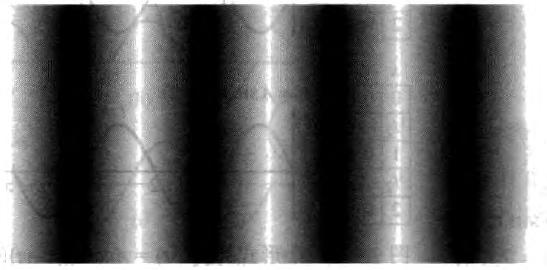
\includegraphics[height=120pt]{assets/1,2/image (41).jpg}
    \caption{\bfseries 空间频率较低的正弦亮度分布 }
\end{subfigure}\begin{subfigure}[t]{0.37\columnwidth}\centering
    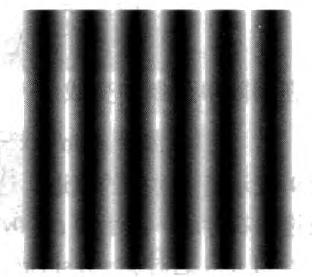
\includegraphics[height=120pt]{assets/1,2/image (42).jpg}
    \caption{\bfseries 空间频率较高的正弦亮度分布 }
\end{subfigure}
\caption{\bfseries 正弦亮度分布 }
\end{figure}

\section{复数表示}
在之后的学习会看到,用余弦或正弦函数描述波函数会带来很多不便,而复数表示在大多时候显得尤为有效,因此引入复数表示是极有必要的。在本书中,为表示某个变量(物理量)是复数,我们在其上加一波浪号,例如 $\tilde{z}$ 或 $\tilde{E}$。

习惯上,我们用复数的实部来描述谐波,例如将 $\psi = A \cos(kx - wt + \varepsilon)$ 写为 $\psi = \Re [A e^{i (kx - wt + \varepsilon)}]$。
为了方便,常常把 $\Re$ 省略不写,即:
\begin{equation}
    \psi(x,t) = A e^{i \theta} = A e^{i (kx - wt + \varepsilon)}
\end{equation}
在后文,我们也采用此简写。需要时刻谨记,真实的波是实部,虚部没有物理意义。

另外,虽然复数表示在物理中十分常见,但应用它时需要时刻小心,只有运算限于加法、减法、乘除实数、对实变量进行微分和积分时,才能恢复实部。乘法运算(包括数乘、点乘和叉乘)必须仅与实数进行,否则会得到错误结论\footnote{这里有一个疑问,在 \ref{全反射时的相位变化} 节(全反射时的相位变化),推导反射光相位变化时,我们利用了 $\boldsymbol{E_r} = \boldsymbol{E_i}\cdot \lambda e^{i \delta} $ 所带来的相位变化,如何保证或说明这样做能得到正确的结果?}。例如 $\Re \tilde{z}_1 \cdot \Re \tilde{z}_2 \ne \Re (\tilde{z}_1\cdot \tilde{z}_2)$,$\Re \boldsymbol{\tilde{A}_1 }\cdot \Re \boldsymbol{\tilde{A}_2 }\ne \Re (\boldsymbol{\tilde{A}_1} \cdot \boldsymbol{\tilde{A}_2})$。

\section{相矢量}\label{相矢量}

相矢量(也称复振幅、旋转矢量)是将谐波 $\psi = A e^{i (kx - wt + \varepsilon)}$ 中的位置变量 $x$ 或时间变量 $t$ 分离出来,以得到复平面上的矢量,常用于计算振幅\footnote{我们将在 3.1 节讨论波的叠加时使用相矢量,并讨论相矢量相加时所代表的意义}等。

\subsection{分离 $x$ 并随 $t$ 旋转}

考虑谐波 $\psi = \psi_0 e^{i(kx - \omega t + \varepsilon)}$,对于任意给定的 $x$,令 $\alpha = kx + \varepsilon$,谐波可写为 $\psi = \psi_0 e^{i(- wt + \alpha)} = (\psi_0 e^{i \alpha})\cdot e^{i(- wt)} $ 是 $t$ 的函数,则此时的相矢量定义为 $ \psi_0 \measuredangle \alpha = \psi_0 e^{i \alpha}$,也常记为 $\psi_0 \angle \alpha$。

相矢量是复平面中的一个矢量(即一个复数),$\psi_0$ 表示其模长,$\alpha$ 表示其幅角,真实的波是它在实轴上的投影。对于 $\psi = \psi_0 e^{i(- wt + \alpha)} $,随着 $t$ 增大,波的相位减小,代表相矢量在复平面中顺时针旋转,$\omega t$ 即为沿顺时针旋转的角度。对于 $\psi = \psi_0 e^{i( wt + \alpha)}$(也即沿 $x$ 轴负方向传播的波),相矢量在复平面中逆时针旋转,$\omega t$ 即为沿逆时针转过的角度。也就是说,将 $x$(以及初相 $\varepsilon$)分离为相矢量后,我们可以方便的研究 $x$ 这一点上,波关于时间 $t$ 的变化情况。

当然,对于波的正弦表示 $\psi = A \sin (kx - wt + \varepsilon)$,也可令  $\alpha = kx + \varepsilon$,得到相矢量 $\psi_0 \measuredangle \alpha = \psi_0 e^{i \alpha}$,只不过此时真实的波是它在虚轴上的投影。

例如,振动 $E_1 = 5 \cos (-\omega t)$,$E_2 = 10 \sin (\omega t + \frac{\pi}{3} )$ 的相矢量分别为 $5 \measuredangle 0$,$10 \measuredangle \frac{\pi}{3} $,前者顺时针旋转,向实轴投影,后者逆时针旋转,向虚轴投影。

\subsection{分离 $t$ 并随 $x$ 旋转}

类似地,考虑谐波 $\psi = \psi_0 e^{i(kx \pm \omega t + \varepsilon)}$。对于任意给定的 $t$,令 $\alpha = \pm \omega t + \varepsilon$,谐波可写为 $\psi = \psi_0 e^{i(kx + \alpha)} = (\psi_0 e^{i \alpha})\cdot e^{i(kx)} $ 是 $x$ 的函数,则此时的相矢量定义为 $ \psi_0 \measuredangle \alpha = \psi_0 e^{i \alpha}$。将 $t$ 分离为相矢量后,我们可以方便的研究 $t$ 这一时刻,波关于位置 $x$ 的变化情况。

习惯上,我们只考虑 $\psi_0 e^{i(kx + \alpha)}$,而不考虑 $\psi_0 e^{i(-kx + \alpha)}$ 的情况,后者可以通过三角变换,等价的改变初相 $\phi_0$ 的值转化为前者。 

例如,对振动 $E_3 = 5 \cos (kx)$,$E_4 = 10 \sin (kx + \frac{\pi}{2} )$,其相矢量分别为 $5 \measuredangle 0$,$10 \measuredangle \frac{\pi}{2} $,两者都逆时针旋转,前者向实轴投影,后者向虚轴投影。



\section{三维波动方程}\label{波动方程}

在介绍波动方程之前,先给出本文默认的一些符号规定,以及一些运算符的定义。

\subsection{内积、叉乘与矩阵乘法}

在本文,一切矢量运算皆使用矩阵运算。并且,若无特殊说明,矢量都等价于列向量,也即下面两种写法等价:
\begin{equation}
    \boldsymbol{A} = (A_x, A_y, A_z),\quad \boldsymbol{A} = \begin{bmatrix} A_x \\ A_y \\ A_z \end{bmatrix}
\end{equation}

用点乘符号 `$\cdot$' 表示两向量的内积,例如 $\boldsymbol{A_1} = (A_{1,x}, A_{2,x}, A_{3,x})$,$\boldsymbol{A_2} = (A_{1,y}, A_{2,y}, A_{3,y})$,则:
\begin{equation}
    \boldsymbol{A_1} \cdot \boldsymbol{A_2} = (A_{1,x}, A_{2,x}, A_{3,x})\cdot (A_{1,y}, A_{2,y}, A_{3,y}) = 
    \begin{bmatrix}
        A_{1,x} \\ A_{2,x} \\ A_{3,x}
    \end{bmatrix}\cdot
    \begin{bmatrix}
        A_{1,y} \\ A_{2,y} \\ A_{3,y}
    \end{bmatrix} =
    A_{1,x}A_{1,y} + A_{2,x}A_{2,y} + A_{3,x}A_{3,y}
\end{equation}
在后文,点乘符号 `$\cdot$' 皆表示内积,叉乘符号 `$\times$' 表示外积,矩阵乘法不用特殊符号,如有必要会使用 `$\odot $' 来表示矩阵乘法。


\subsection{微分算子}

下面依次给出微分算子 $\nabla$、拉普拉斯算子 $\Delta$ 和矢量微分的定义。

假设 $f = f(\boldsymbol{x})$ 是三维空间中的标量函数,$\boldsymbol{A} = \boldsymbol{A}(\boldsymbol{x}) = \left( A_x(\boldsymbol{x}), A_y(\boldsymbol{x}), A_z(\boldsymbol{x}) \right)$ 是三维空间中的矢量(数学上称为自变量为 3 维的 3 维向量值函数),设 $\boldsymbol{B} = \boldsymbol{B}(\boldsymbol{x}) \left( \boldsymbol{B_1}(x,y,z), \boldsymbol{B_1}(x,y,z), \boldsymbol{B_1}(x,y,z) \right)$ 是三个矢量构成的张量(可视为 $3 \times 3$ 矩阵),如下:
\begin{align}
    f &= f(\boldsymbol{x}) = f(x,y,z) 
    \\ 
    \boldsymbol{A} &= \boldsymbol{A}(\boldsymbol{x})  = 
    \begin{bmatrix}
        A_x(\boldsymbol{x}) \\ A_y(\boldsymbol{x}) \\ A_z(\boldsymbol{x})
    \end{bmatrix}=
    \begin{bmatrix}
        A_x(x,y,z) \\ A_y(x,y,z) \\ A_z(x,y,z)
    \end{bmatrix}
    \\ 
    \boldsymbol{B} &= \boldsymbol{B}(\boldsymbol{x}) = 
    \begin{bmatrix}
        \boldsymbol{B_1}(\boldsymbol{x}) \\ \boldsymbol{B_2}(\boldsymbol{x}) \\ \boldsymbol{B_3}(\boldsymbol{x})
    \end{bmatrix} = 
    \begin{bmatrix}
        B_{1,x}(\boldsymbol{x}) & B_{1,y}(\boldsymbol{x}) & B_{1,z}(\boldsymbol{x})\\ 
        B_{2,x}(\boldsymbol{x}) & B_{2,y}(\boldsymbol{x}) & B_{2,z}(\boldsymbol{x})\\
        B_{3,x}(\boldsymbol{x}) & B_{3,y}(\boldsymbol{x}) & B_{3,z}(\boldsymbol{x})
    \end{bmatrix}
\end{align}

定义微分算子 $\nabla$: 
\begin{equation}
    \begin{aligned}
        &\text{微分算子:} 
        &&\nabla = 
        \begin{bmatrix}
            \frac{\partial  }{\partial x }, \frac{\partial  }{\partial y }, \frac{\partial  }{\partial z }
        \end{bmatrix}
        \\ 
        &\text{梯度:} &&\nabla f = 
        \begin{bmatrix}
            \frac{\partial f }{\partial x }, \frac{\partial f }{\partial y }, \frac{\partial f }{\partial z }
        \end{bmatrix}\\ 
        &\text{广义梯度:}
        &&\nabla \boldsymbol{A} = 
        \begin{bmatrix}
            \nabla A_x \\ \nabla A_y \\ \nabla A_z
        \end{bmatrix} = 
        \begin{bmatrix}
            \frac{\partial A_x }{\partial x } & \frac{\partial A_x }{\partial y } & \frac{\partial A_x }{\partial z } \\
            \frac{\partial A_y }{\partial x } & \frac{\partial A_y }{\partial y } & \frac{\partial A_y }{\partial z } \\
            \frac{\partial A_z }{\partial x } & \frac{\partial A_z }{\partial y } & \frac{\partial A_z }{\partial z }
        \end{bmatrix}_{3 \times 3}
    \end{aligned}    
\end{equation}
\begin{equation}
\begin{aligned}
    &\text{旋度:}
    &&\nabla \cdot \boldsymbol{A} 
    =
    \begin{bmatrix}
        \frac{\partial  }{\partial x }, \frac{\partial  }{\partial y }, \frac{\partial  }{\partial z }
    \end{bmatrix}
    \cdot 
    \begin{bmatrix}
        A_x \\ A_y \\ A_z
    \end{bmatrix} 
    = 
    \frac{\partial A_x }{\partial x } +\frac{\partial A_y }{\partial y } + \frac{\partial A_z }{\partial z }
    \\ 
    &\text{广义旋度:}
    &&\nabla \cdot \boldsymbol{B} = 
    \nabla \cdot 
    \begin{bmatrix}
        \boldsymbol{B_1} \\ \boldsymbol{B_2} \\ \boldsymbol{B_3}
    \end{bmatrix} = 
    \begin{bmatrix}
        \nabla \cdot \boldsymbol{B_1} \\ \nabla \cdot \boldsymbol{B_2} \\ \nabla \cdot \boldsymbol{B_3}
    \end{bmatrix} = 
    \begin{bmatrix}
        \frac{\partial B_{1,x} }{\partial x } +\frac{\partial B_{1,y} }{\partial y } + \frac{\partial B_{1,z} }{\partial z } \\
        \frac{\partial B_{2,x} }{\partial x } +\frac{\partial B_{2,y} }{\partial y } + \frac{\partial B_{2,z} }{\partial z } \\
        \frac{\partial B_{3,x} }{\partial x } +\frac{\partial B_{3,y} }{\partial y } + \frac{\partial B_{3,z} }{\partial z }
    \end{bmatrix}_{3\times 1}
\end{aligned}
\end{equation}

\subsection{拉普拉斯算子}

并以此定义拉普拉斯算子 $\Delta$: 
\begin{gather}
\begin{aligned}
    &\text{拉普拉斯算子:}
    &&\Delta = \nabla \cdot (\nabla \ \ \ ) 
    =  
    \begin{bmatrix}
        \frac{\partial  }{\partial x }, \frac{\partial  }{\partial y }, \frac{\partial  }{\partial z }
    \end{bmatrix} \cdot 
    \begin{bmatrix}
        \frac{\partial  }{\partial x }, \frac{\partial  }{\partial y }, \frac{\partial  }{\partial z }
    \end{bmatrix}
    = 
    \frac{\partial^2 }{\partial x^2 } +\frac{\partial^2 }{\partial y^2 } + \frac{\partial^2 }{\partial z^2 } \\ 
    &\text{拉普拉斯运算:} &&\Delta f = \nabla^2 f = \nabla \cdot (\nabla f ) 
    = 
    \begin{bmatrix}
        \frac{\partial  }{\partial x }, \frac{\partial  }{\partial y }, \frac{\partial  }{\partial z }
    \end{bmatrix} 
    \cdot 
    \begin{bmatrix}
        \frac{\partial f }{\partial x }, \frac{\partial f }{\partial y }, \frac{\partial f }{\partial z }
    \end{bmatrix}
    =
    \frac{\partial^2 f }{\partial x^2 } +\frac{\partial^2 f }{\partial y^2 } + \frac{\partial^2 f }{\partial z^2 } 
\end{aligned}
\end{gather}
\begin{gather}
\begin{aligned}
    &\text{广义拉普运算:}
    &&\Delta \boldsymbol{A}  = \nabla \cdot (\nabla \boldsymbol{A} ) 
    =
    \nabla \cdot 
    \begin{bmatrix}
        \nabla A_x \\ \nabla A_y \\ \nabla A_z
    \end{bmatrix} 
    = 
    \begin{bmatrix}
        \nabla \cdot (\nabla A_x) \\ \nabla \cdot (\nabla A_y) \\ \nabla \cdot (\nabla A_z)
    \end{bmatrix} 
    =
    \begin{bmatrix}
        \frac{\partial^2 A_x }{\partial x^2 } +\frac{\partial^2 A_x }{\partial y^2 } + \frac{\partial^2 A_x }{\partial z^2 } \\
        \frac{\partial^2 A_y }{\partial x^2 } +\frac{\partial^2 A_y }{\partial y^2 } + \frac{\partial^2 A_y }{\partial z^2 } \\
        \frac{\partial^2 A_z }{\partial x^2 } +\frac{\partial^2 A_z }{\partial y^2 } + \frac{\partial^2 A_z }{\partial z^2 }
    \end{bmatrix}_{3\times 1} \\ 
    & \text{也可理解为:} &&
    \Delta \boldsymbol{A} = 
    \Delta \begin{bmatrix}
        A_x \\ A_y \\ A_z
    \end{bmatrix} = 
    \begin{bmatrix}
        \Delta A_x \\ \Delta A_y \\ \Delta A_z
    \end{bmatrix}
    = 
    \begin{bmatrix}
        \frac{\partial^2 A_x }{\partial x^2 } +\frac{\partial^2 A_x }{\partial y^2 } + \frac{\partial^2 A_x }{\partial z^2 } \\
        \frac{\partial^2 A_y }{\partial x^2 } +\frac{\partial^2 A_y }{\partial y^2 } + \frac{\partial^2 A_y }{\partial z^2 } \\
        \frac{\partial^2 A_z }{\partial x^2 } +\frac{\partial^2 A_z }{\partial y^2 } + \frac{\partial^2 A_z }{\partial z^2 }
    \end{bmatrix}_{3\times 1}
\end{aligned}
\end{gather}

例如,对于三维空间中的矢量 $\boldsymbol{E} = \boldsymbol{E}(\boldsymbol{x}) = \left( E_x(\boldsymbol{x}), E_y(\boldsymbol{x}), E_z(\boldsymbol{x})  \right)$,我们有:
\begin{equation}
    \Delta \boldsymbol{E}  = \nabla \cdot (\nabla \boldsymbol{E} ) 
    =
    \nabla \cdot 
    \begin{bmatrix}
        \nabla E_x \\ \nabla E_y \\ \nabla E_z
    \end{bmatrix} 
    = 
    \begin{bmatrix}
        \nabla \cdot (\nabla E_x) \\ \nabla \cdot (\nabla E_y) \\ \nabla \cdot (\nabla E_z)
    \end{bmatrix} 
    =
    \begin{bmatrix}
        \frac{\partial^2 E_x }{\partial x^2 } +\frac{\partial^2 E_x }{\partial y^2 } + \frac{\partial^2 E_x }{\partial z^2 } \\
        \frac{\partial^2 E_y }{\partial x^2 } +\frac{\partial^2 E_y }{\partial y^2 } + \frac{\partial^2 E_y }{\partial z^2 } \\
        \frac{\partial^2 E_z }{\partial x^2 } +\frac{\partial^2 E_z }{\partial y^2 } + \frac{\partial^2 E_z }{\partial z^2 }
    \end{bmatrix}_{3\times 1}
\end{equation}

\subsection{矢量微分}

\begin{gather}
    \frac{\partial \boldsymbol{A} }{\partial x } = \frac{\partial  }{\partial x }\boldsymbol{A} = 
    \frac{\partial  }{\partial x } 
    \begin{bmatrix}
        A_x \\ A_y \\ A_z
    \end{bmatrix} = 
    \begin{bmatrix}
        \frac{\partial A_x }{\partial x } \\ \frac{\partial A_y }{\partial x } \\ \frac{\partial A_z }{\partial x }
    \end{bmatrix} 
    ,\quad 
    \frac{\partial^2 \boldsymbol{A} }{\partial x^2 } = 
    \frac{\partial^2  }{\partial x^2 } \boldsymbol{A} = 
    \frac{\partial^2  }{\partial x^2 } 
    \begin{bmatrix}
        A_x \\ A_y \\ A_z
    \end{bmatrix} = 
    \begin{bmatrix}
        \frac{\partial^2 A_x }{\partial x^2 } \\ \frac{\partial^2 A_y }{\partial x^2 } \\ \frac{\partial^2 A_z }{\partial x^2 }
    \end{bmatrix}
\end{gather}

\subsection{波动方程}

定义好上述工具后,可以给出三维空间中的波动方程:
\begin{equation}
    \Delta \boldsymbol{\psi} =\frac{1}{v^{2}}\frac{\partial^{2}\boldsymbol{\psi}}{\partial t^{2}}
\end{equation}
例如,对矢量 $\boldsymbol{E}$,上面方程表示:
\begin{equation}
    \Delta \boldsymbol{E} =\frac{1}{v^{2}}\frac{\partial^{2}\boldsymbol{E}}{\partial t^{2}} 
    \Longleftrightarrow 
    \begin{bmatrix}
        \Delta E_x \\ 
        \Delta E_y \\
        \Delta E_z
    \end{bmatrix} = 
    \frac{1}{v^{2}}
    \begin{bmatrix}
        \frac{\partial^{2}E_x}{\partial t^{2}} \\ 
        \frac{\partial^{2}E_y}{\partial t^{2}} \\
        \frac{\partial^{2}E_z}{\partial t^{2}}
    \end{bmatrix} 
    \Longleftrightarrow
    \begin{cases}
        \Delta E_x =\frac{1}{v^{2}}\frac{\partial^{2}E_x}{\partial t^{2}}\\
        \Delta E_y =\frac{1}{v^{2}}\frac{\partial^{2}E_y}{\partial t^{2}}\\
        \Delta E_z =\frac{1}{v^{2}}\frac{\partial^{2}E_z}{\partial t^{2}}
    \end{cases}
\end{equation}
上面几种表示是等价的。


\section{平面波、柱面波与球面波}\label{平面波、柱面波与球面波}

平面波、柱面波与球面波是最具有实际意义的波形,因为它们在现实中最容易实现\footnote{其推导详见参考文献 \cite{Optics} 的 Page 47-56,以及 \href{https://zhuanlan.zhihu.com/p/693746762}{知乎:电磁波的平面波、柱面波和球面波的表达式与推导 (https://zhuanlan.zhihu.com/p/693746762)},这里不多赘述}。

\subsection{平面波}

三维空间中的平面波\footnote{平面波概念的引入详见参考文献 \cite{Optics} 的 Page 30,这里不再赘述}:
\begin{equation}
\boldsymbol{\psi}(\boldsymbol{x}, t) = \boldsymbol{A}\cdot e^{i(\boldsymbol{k}\cdot \boldsymbol{x} \mp \omega t + \varepsilon)}
\end{equation}

每个等相面由下式给出:
\begin{equation}
    \boldsymbol{k} \cdot \boldsymbol{x} = \text{const}
\end{equation}

此扰动的每个等相面(也称波阵面)都是一个平面,且波矢 $\boldsymbol{k}$ 垂直于等相面,$(\boldsymbol{k}\cdot \boldsymbol{x} - \omega t)$ 时沿 $\boldsymbol{k}$ 传播,$(\boldsymbol{k}\cdot \boldsymbol{x} + \omega t)$ 时沿 $\boldsymbol{k}$ 的反方向传播。在一切三维波中,只有平面波(可以是谐波也可以是非谐波)穿过空间传播时其截面轮廓(等相面)保持不变。

有时,$\boldsymbol{A}$ 是 $\boldsymbol{x}$ 的函数,称为非均匀波(例如 2.5 节介绍的隐失波)。

\subsection{球面波}

在球坐标系 $(r, \phi, \theta)$ 下,可以解得球面波方程:
\begin{equation}
\boldsymbol{\psi} = \boldsymbol{\psi}(\boldsymbol{r}, t) = \boldsymbol{\psi_{0}}(r) \cdot e^{i\left( k r \mp  \omega t + \varepsilon \right)} =  \frac{\boldsymbol{A}}{r}\cdot e^{i\left( k r \mp  \omega t + \varepsilon \right)}
\end{equation}

每个波阵面(等相面)由下式给出:
\begin{equation}
kr = \text{const}
\end{equation}

注意,任何球面波的振幅 $\boldsymbol{\psi_0}$ 都是 $r$ 的函数,因为球面波的振幅随着距离的增加而减小(能量守恒的必然结果)。当它从原点向外传播时,波阵面是逐渐扩张为更大的圆。

\subsection{柱面波}

在柱坐标系 $(r, \theta, z)$ 下,可以解得柱面波方程:
\begin{equation}
\boldsymbol{\psi} = \boldsymbol{\psi}(\boldsymbol{r}, t) = \boldsymbol{\psi_{0}}(r) \cdot e^{i\left( k r \mp  \omega t + \varepsilon \right)} = \frac{\boldsymbol{A}}{\sqrt{r}}\cdot e^{i\left( kr \mp  \omega t + \varepsilon \right)}
\end{equation}

每个等相面由下式给出:
\begin{equation}
    kr = \text{const}
\end{equation}

平面波投射到具有细长狭缝的不透明屏幕上,就会通过此狭缝发出与柱面波相似的扰动,目前大多采用此方法产生柱面光波。






\chapter*{附录 B\hspace*{20pt}  Matlab 代码}\addcontentsline{toc}{chapter}{附录 B\hspace*{6pt}  Matlab 代码}   
\thispagestyle{fancy} 
\setcounter{section}{0}   
\renewcommand\thesection{B.\arabic{section}}   
\renewcommand{\thefigure}{B.\arabic{figure}} 
\renewcommand{\thetable}{B.\arabic{table}}

\section{图 \ref{振幅系数随入射角的变化} 源码}
\begin{matlablisting}
%%%%%%%%%% 空气入射玻璃 %%%%%%%%%%
global n_i n_t
n_i = 1;
n_t = 1.5;

theta_t = @(theta_i) asin(n_i/n_t*sin(theta_i));
r_s = @(theta_i, theta_t) - sin(theta_i - theta_t)./sin(theta_i + theta_t);
r_p = @(theta_i, theta_t) + tan(theta_i - theta_t)./tan(theta_i + theta_t);
t_s = @(theta_i, theta_t) 2*sin(theta_t).*cos(theta_i)./sin(theta_i + theta_t);
t_p = @(theta_i, theta_t) 2*sin(theta_t).*cos(theta_i) ./ ( sin(theta_i + theta_t).*cos(theta_i - theta_t) );
theta_B = atan(n_t/n_i);
theta_C = asin(n_t/n_i);

theta_array = linspace(-0.1, pi/2, 101);
Y = [
    r_s(theta_array, theta_t(theta_array))
    r_p(theta_array, theta_t(theta_array))
    t_s(theta_array, theta_t(theta_array))
    t_p(theta_array, theta_t(theta_array))
    ];
stc = MyPlot(theta_array, Y);
xline(theta_B, 'b')
yline(0)
xlim([0, pi/2])
ylim([-1, 1])
stc.leg.String = ["$r_s$"; "$r_p$"; "$t_s$"; "$t_p$"; "$\theta_i = \theta_B$"];
stc.leg.Interpreter = "latex";
stc.leg.FontSize = 14;
stc.leg.Location = "southwest";
stc.axes.Title.String = '$n_i = 1 < n_t = 1.5$';
stc.axes.Title.Interpreter = "latex";
stc.label.x.String = '$\theta_i$';
stc.label.y.String = '$r$';
stc.plot.plot_3.LineStyle = ":";
stc.plot.plot_3.Color = 'b';
stc.plot.plot_4.LineStyle = ":";
stc.plot.plot_4.Color = [1 0 1];
%MyExport_pdf

%%%%%%%%%% 玻璃入射空气 %%%%%%%%%%
n_i = 1.5;
n_t = 1;

theta_t = @(theta_i) asin(n_i/n_t*sin(theta_i));
r_s = @(theta_i, theta_t) - sin(theta_i - theta_t)./sin(theta_i + theta_t);
r_p = @(theta_i, theta_t) + tan(theta_i - theta_t)./tan(theta_i + theta_t);
t_s = @(theta_i, theta_t) 2*sin(theta_t).*cos(theta_i)./sin(theta_i + theta_t);
t_p = @(theta_i, theta_t) 2*sin(theta_t).*cos(theta_i) ./ ( sin(theta_i + theta_t).*cos(theta_i - theta_t) );
theta_B = atan(n_t/n_i);
theta_C = asin(n_t/n_i);


theta_array = linspace(0, theta_C, 101);
Y = [
    r_s(theta_array, theta_t(theta_array))
    r_p(theta_array, theta_t(theta_array))
    t_s(theta_array, theta_t(theta_array))
    t_p(theta_array, theta_t(theta_array))
    ];
stc = MyPlot(theta_array, Y);
xline(theta_B, 'b')
xline(theta_C, 'r')
yline(0)
xlim([0, pi/2])
ylim([-0.5, 3])
stc.leg.String = ["$r_s$"; "$r_p$"; "$t_s$"; "$t_p$"; "$\theta_i = \theta_B$"; "$\theta_i = \theta_C$"];
stc.leg.Interpreter = "latex";
stc.axes.Title.String = '$n_i = 1.5 > n_t = 1$';
stc.axes.Title.Interpreter = "latex";
stc.label.x.String = '$\theta_i$';
stc.label.y.String = '$r$';
stc.plot.plot_3.LineStyle = ":";
stc.plot.plot_3.Color = 'b';
stc.plot.plot_4.LineStyle = ":";
stc.plot.plot_4.Color = [1 0 1];
%MyExport_pdf
\end{matlablisting}

\section{图 \ref{反射折射光的振幅与能量变化} 源码}
\label{反射折射光的振幅与能量变化 源码}
\begin{matlablisting}
global n_i n_t
%%%%%%%%%% 反射折射光振幅与能量变化 (空气入射玻璃) %%%%%%%%%%
MyColor = num2cell( ...
    [
"#ff8080" "#ff0000" "#990000" "#190000"
"#80ff80" "#00ff00" "#009900" "#001900"
"#8080ff" "#0000ff" "#000099" "#000019"
"#ff80ff" "#ff00ff" "#990099" "#190019"
"#ffff80" "#ffff00" "#999900" "#191900"
"#80ffff" "#00ffff" "#009999" "#001919"
"#ffffff" "#bbbbbb" "#999999" "#191919"
    ]...
);
n_i = 1;
n_t = 1.5;

theta_t = @(theta_i) asin(n_i/n_t*sin(theta_i));
r_s = @(theta_i, theta_t) - sin(theta_i - theta_t)./sin(theta_i + theta_t);
r_p = @(theta_i, theta_t) + tan(theta_i - theta_t)./tan(theta_i + theta_t);
t_s = @(theta_i, theta_t) 2*sin(theta_t).*cos(theta_i)./sin(theta_i + theta_t);
t_p = @(theta_i, theta_t) 2*sin(theta_t).*cos(theta_i) ./ ( sin(theta_i + theta_t).*cos(theta_i - theta_t) );
theta_B = atan(n_t/n_i);
theta_C = asin(n_t/n_i);

theta_array_2 = linspace(-0.1, pi/2, 101);
Y = [
    r_s(theta_array_2, theta_t(theta_array_2))
    r_p(theta_array_2, theta_t(theta_array_2))
    t_s(theta_array_2, theta_t(theta_array_2))
    t_p(theta_array_2, theta_t(theta_array_2))
    r_s(theta_array_2, theta_t(theta_array_2)).^2
    r_p(theta_array_2, theta_t(theta_array_2)).^2
    0.5 * ( r_s(theta_array_2, theta_t(theta_array_2)).^2 + r_p(theta_array_2, theta_t(theta_array_2)).^2 )
    ];

stc = MyPlot(theta_array_2, Y);
yline(0, 'black', 'Alpha', 1, 'LineWidth', 1)
xline(theta_B,'Color', [0 1 1], 'Alpha', 1, 'LineWidth', 0.7)
xlim([0, pi/2])
ylim([-1, 1])
    stc.leg.Interpreter = 'latex';
    stc.leg.FontSize = 15;
    stc.leg.Location = 'southwest';
    stc.axes.Title.String = '$n_i = 1 < n_t = 1.5$';
    stc.axes.Title.Interpreter = 'latex';
    stc.label.x.String = '$\theta_i$';
    stc.label.y.String = '$y$';
    %stc.leg.String = ["$y=r_s$"; "$y=r_p$"; "$y=t_s$"; "$y=t_p$"; "$y=R_s$"; "$y=R_p$"; "$y=R$"; "$y=0$";  "$\theta_i = \theta_B$";];
    stc.leg.Visible = 'off';

    stc.plot.plot_2.LineStyle = "-";
    stc.plot.plot_3.LineStyle = ":";
    stc.plot.plot_4.LineStyle = ":";
    stc.plot.plot_5.LineStyle = "--";
    %stc.plot.plot_5.LineWidth = 0.7;
    stc.plot.plot_6.LineStyle = "--";
    %stc.plot.plot_6.LineWidth = 0.7;
    stc.plot.plot_7.LineStyle = "-";

    stc.plot.plot_1.Color = MyColor{4, 2};
    stc.plot.plot_3.Color = MyColor{4, 1};
    stc.plot.plot_5.Color = MyColor{4, 3};
    stc.plot.plot_2.Color = MyColor{3, 2};
    stc.plot.plot_4.Color = MyColor{3, 1};
    stc.plot.plot_6.Color = MyColor{3, 3}; 
    stc.plot.plot_7.Color = [1 0 0];   
%MyExport_pdf
%MyExport_pdf_docked
%MyExport_svg_docked


%%%%%%%%%% 反射折射光振幅与能量变化 (玻璃入射空气) %%%%%%%%%%
n_i = 1.5;
n_t = 1;

theta_t = @(theta_i) asin(n_i/n_t*sin(theta_i));
r_s = @(theta_i, theta_t) - sin(theta_i - theta_t)./sin(theta_i + theta_t);
r_p = @(theta_i, theta_t) + tan(theta_i - theta_t)./tan(theta_i + theta_t);
t_s = @(theta_i, theta_t) 2*sin(theta_t).*cos(theta_i)./sin(theta_i + theta_t);
t_p = @(theta_i, theta_t) 2*sin(theta_t).*cos(theta_i) ./ ( sin(theta_i + theta_t).*cos(theta_i - theta_t) );
theta_B = atan(n_t/n_i);
theta_C = asin(n_t/n_i);

theta_array_2 = linspace(-0.1, theta_C, 250);
theta_array_all = [linspace(-0.1, 0.65, 100), linspace(0.65, 0.74, 50), linspace(0.74, pi/2, 100)];

X = [
    theta_array_all
    theta_array_all
    theta_array_all
    theta_array_all
    theta_array_all
    theta_array_all
    theta_array_all
];

Y = [
    (theta_array_all < theta_C).*r_s(theta_array_all, theta_t(theta_array_all)) + (theta_array_all > theta_C).*abs(r_s(theta_array_all, theta_t(theta_array_all)))
    (theta_array_all < theta_C).*r_p(theta_array_all, theta_t(theta_array_all)) + (theta_array_all > theta_C).*abs(r_p(theta_array_all, theta_t(theta_array_all)))
    abs( t_s(theta_array_all, theta_t(theta_array_all)) )
    abs( t_p(theta_array_all, theta_t(theta_array_all)) )
    abs(r_s(theta_array_all, theta_t(theta_array_all))).^2
    abs(r_p(theta_array_all, theta_t(theta_array_all))).^2
    0.5 * (  abs(r_s(theta_array_all, theta_t(theta_array_all))).^2 + abs(r_p(theta_array_all, theta_t(theta_array_all))).^2   )
    ];

stc = MyPlot(X, Y);
yline(0, 'black', 'Alpha', 1, 'LineWidth', 1)
xline(theta_B,'Color', [0 1 1], 'Alpha', 1, 'LineWidth', 0.7)
xline(theta_C,'Color', [0 1 0], 'Alpha', 1, 'LineWidth', 0.7)
xlim([0, pi/2])
ylim([-0.5, 3])
    stc.leg.Interpreter = 'latex';
    stc.leg.FontSize = 14;
    stc.leg.Location = 'northwestoutside';
    stc.axes.Title.String = '$n_i = 1 < n_t = 1.5$';
    stc.axes.Title.Interpreter = "latex";
    stc.label.x.String = '$\theta_i$';
    stc.label.y.String = '$y$';
    stc.leg.String = ["$y=r_s$"; "$y=r_p$"; "$y=t_s$"; "$y=t_p$"; "$y=R_s$"; "$y=R_p$"; "$y=R$"; "$y=0$";  "$\theta_i = \theta_B$"; "$\theta_i = \theta_C$";];
    
    stc.plot.plot_2.LineStyle = "-";
    stc.plot.plot_3.LineStyle = ":";
    stc.plot.plot_4.LineStyle = ":";
    stc.plot.plot_5.LineStyle = "--";
    %stc.plot.plot_5.LineWidth = 0.7;
    stc.plot.plot_6.LineStyle = "--";
    %stc.plot.plot_6.LineWidth = 0.7;
    stc.plot.plot_7.LineStyle = "-";

    stc.plot.plot_1.Color = MyColor{4, 2};
    stc.plot.plot_3.Color = MyColor{4, 1};
    stc.plot.plot_5.Color = MyColor{4, 3};
    stc.plot.plot_2.Color = MyColor{3, 2};
    stc.plot.plot_4.Color = MyColor{3, 1};
    stc.plot.plot_6.Color = MyColor{3, 3}; 
    stc.plot.plot_7.Color = [1 0 0];   
%MyExport_pdf
%MyExport_pdf_docked
%MyExport_svg_docked
\end{matlablisting}

\section{图 \ref{反射光 s 分量与 p 分量的相位增量} 源码}
\label{反射光 s 分量与 p 分量的相位增量 源码}
\begin{matlablisting}
global n_i n_t n_ti theta_B theta_C 

%%%%%%%%%% 反射光相位增量 (空气入射玻璃) %%%%%%%%%%
n_i = 1;
n_t = 1.5;
n_ti = n_t/n_i;
theta_B = atan(n_ti);

theta_array_2 = linspace(0, pi/2-0.001, 200);

delta_r_s = @(t) -pi ;
delta_r_p = @(t) (-pi).*(t > theta_B).*( t <pi/2);

delta_r_s_kongqi = delta_r_s(theta_array_2);
delta_r_p_kongqi = delta_r_p(theta_array_2);

Y = [
    zeros(size(theta_array_2)) - pi;
    delta_r_p_kongqi;    
];

stc1 = MyPlot(theta_array_2, Y([1 2], :));
xlim([0, pi/2])
yline(0, 'black', 'Alpha', 1, 'LineWidth', 0.5)
xline(theta_B,'Color', [0 1 1], 'Alpha', 1, 'LineWidth', 0.5)
xline(pi/2, '--');
stc1.plot.plot_2.LineStyle = '--';
stc1.leg.String = ["$\delta = \delta_{r,s}$"; "$\delta = \delta_{r,p}$"; "$\delta = 0$"; "$\theta_i = \theta_B$";];
stc1.label.x.String = '$\theta_i$';
stc1.label.y.String = '$\delta$';
stc1.axes.Title.Interpreter = 'latex';
stc1.axes.Title.String = '$n_i = 1 < n_t = 1.5$';
%MyExport_pdf

%%%%%%%%%% 反射光相位增量 (玻璃入射空气) %%%%%%%%%%
n_i = 1.5;
n_t = 1;
n_ti = n_t/n_i;
theta_B = atan(n_ti);
theta_C = asin(n_ti);


delta_r_s = @(t) (t>theta_C).*2.*atan( -(sqrt(sin(t).^2 - n_ti^2))./cos(t) ) ;
delta_r_p = @(t) ...
     (t<theta_B).*(-pi) ... 
   + (theta_B<t).*(t<theta_C).*0 ... 
   + (theta_C<t).*( -2*atan( (sqrt(sin(t).^2 - n_ti^2))./(n_ti^2.*cos(t)) ) );

Y = [
    zeros(size(theta_array_2)) - pi;
    delta_r_p_kongqi;
    delta_r_s(theta_array_2);
    delta_r_p(theta_array_2);
];


stc2 = MyPlot(theta_array_2, Y([3 4], :));
xlim([0, pi/2])
yline(0, 'black', 'Alpha', 1, 'LineWidth', 0.5)
xline(theta_B,'Color', [0 1 1], 'Alpha', 1, 'LineWidth', 0.5)
xline(theta_C,'Color', [0 1 0], 'Alpha', 1, 'LineWidth', 0.5)
xline(pi/2, '--');
stc2.plot.plot_2.LineStyle = '--';
stc2.leg.String = ["$\delta = \delta_{r,s}$"; "$\delta = \delta_{r,p}$"; "$\delta = 0$"; "$\theta_i = \theta_B$"; "$\theta_i = \theta_C$";];
stc2.leg.Location = 'northeast';
stc2.label.x.String = '$\theta_i$';
stc2.label.y.String = '$\delta$';
stc2.axes.Title.Interpreter = 'latex';
stc2.axes.Title.String = '$n_i = 1.5 > n_t = 1$';
%MyExport_pdf
\end{matlablisting}

\section{图 \ref{隐失波穿透深度与 GH Shift 玻璃入射空气} 源码}
\label{隐失波穿透深度与 GH Shift 玻璃入射空气 源码}
\begin{matlablisting}
%%%%%%%%%% 隐失波的穿透深度和 GH Shift (玻璃入射空气) %%%%%%%%%%
global lambda n_i n_t
n_i = 1.5;
n_t = 1;
lambda = 550 * 10^(-9);     % 550.0 nm 的绿色光
delta = @(t) 1 ./ ( 2*pi*sqrt( sin(t).^2 - n_ti^2 )/lambda );
Delta_x = @(t) 2*delta(t).*tan(t);

theta_array_1 = linspace(theta_C, pi/2, 200);
theta_array_2 = linspace(theta_C, pi/2-0.05, 200);


X = [
    theta_array_1
    theta_array_2
];
Y = [
    delta(theta_array_1)/lambda
    Delta_x(theta_array_2)/lambda
];

stc = MyPlot(X, Y);
xlim([theta_C - 0.05, pi/2+0.02])
yline(1, 'black', 'Alpha', 1, 'LineWidth', 0.5)
xline(theta_C,'Color', [0 1 0], 'Alpha', 1, 'LineWidth', 0.5)
stc.leg.String = ["$y = \delta / \lambda$"; "$y = \Delta x / \lambda$"; "$y = 1$"; "$\theta_i = \theta_C$"; "$\theta_i = \frac{\pi}{2}$"];
stc.label.x.String = '$\theta_i$';
stc.label.y.String = '$y$';
xlim([theta_C - 0.05, pi/2])

%MyExport_pdf_docked
\end{matlablisting}

\section{图 \ref{单个球面波源在平面上的振荡情况} 源码}
\label{单个球面波源在平面上的振荡情况 源码}

\begin{matlablisting}
%%%%%%%%%% 单个球面波源在平面上的振荡 (导出为 gif) %%%%%%%%%%
clc,clear,close all;
global lambda k omega X_OA A

lambda = 550.0 * 10^(-9); % 单位: m
k = 5;      % k 取决于光的波长,但在可视化中不妨令为 1
omega = 1;  % omega 取决于光的波长,但在可视化中不妨令为 1
X_OA = [ 0, 0];  % 球面波源 A 的位置
A = 50; % r = 1 时的振幅
E_A0 = @(x, y) A./sqrt( (x - X_OA(1)).^2 + (y - X_OA(2)).^2 ); % X 位置的振幅, 输入的 X_array 为一列行向量
alpha_A = @(x, y) k*sqrt( (x - X_OA(1)).^2 + (y - X_OA(2)).^2 );
vib = @(E_0, t, alpha) E_0.*cos(-omega*t + alpha); % 振荡函数

R_array = linspace(2, 10, 100);
theta_array = transpose(linspace(0, 2*pi, 50));
x_matrix = R_array .* cos(theta_array) + X_OA(1);
y_matrix = R_array .* sin(theta_array) + X_OA(2);
E_A0_matrix = E_A0(x_matrix, y_matrix);
alpha_A_matrix = alpha_A(x_matrix, y_matrix);

stc = MyMesh(x_matrix, y_matrix, vib(E_A0_matrix, 0, alpha_A_matrix), 1);
stc.label_left.z.String = '$E$';


figure 
h1 = surf(x_matrix, y_matrix, E_A0_matrix, 'EdgeColor', 'interp', FaceColor='interp');
hold on
surf([X_OA(1) X_OA(1)], [X_OA(2) X_OA(2)], [30 -30; 30 -30])
colormap(redblue);
zlim([-35 35]);
xlim([X_OA(1) - R_array(end), X_OA(1) + R_array(end)])
ylim([X_OA(2) - R_array(end), X_OA(2) + R_array(end)])
drawnow

t_array = linspace(0, 20, 200);
for i = 1:length(t_array)
    h1.ZData = vib(E_A0_matrix, t_array(i), alpha_A_matrix);
    f(i) = getframe(gcf);
end

numFrames = length(t_array);
animated(1,1,1,numFrames) = 0;
for i = 1:numFrames
    if i == 1
        [animated,cmap] = rgb2ind(f(i).cdata,256,'nodither');
    else
        animated(:,:,1,i) = rgb2ind(f(i).cdata,cmap,'nodither');
    end
end
filename = '单个球面波源在平面上的振荡.gif';
imwrite(animated,cmap,filename,'DelayTime',1/30,'LoopCount',inf);
web(filename)
\end{matlablisting}

\section{图 \ref{两个球面波源在平面上的干涉情况} 源码}
\label{两个球面波源在平面上的干涉情况 源码}

\begin{matlablisting}
%%%%%%%%%% 两个球面波源在平面上的干涉情况 (导出为 gif) %%%%%%%%%%

clc, clear, close all;
global lambda k omega X_OA X_OB A B

lambda = 550.0 * 10^(-9); % 单位: m
k = 5;      % k 取决于光的波长,但在可视化中不妨令为 1
omega = 1;  % omega 取决于光的波长,但在可视化中不妨令为 1
X_OA = [-2, 0];  % 球面波源 A 的位置
X_OB = [ 2, 0];  % 球面波源 B 的位置
A = 50; % r = 1 时 A 的振幅
B = 50; % r = 1 时 B 的振幅

E_A0 = @(x, y) A./sqrt( (x - X_OA(1)).^2 + (y - X_OA(2)).^2 ); % X 位置的振幅, 输入的 X_array 为一列行向量
E_B0 = @(x, y) B./sqrt( (x - X_OB(1)).^2 + (y - X_OB(2)).^2 ); % X 位置的振幅, 输入的 X_array 为一列行向量
alpha_A = @(x, y) k*sqrt( (x - X_OA(1)).^2 + (y - X_OA(2)).^2 );
alpha_B = @(x, y) k*sqrt( (x - X_OB(1)).^2 + (y - X_OB(2)).^2 );
E_0 = @(E_A0, alpha_A, E_B0, alpha_B) sqrt( E_A0.^2 + E_B0.^2 + 2*E_A0.*E_B0.*cos(alpha_A - alpha_B) );
vib = @(E_0, t, alpha) E_0.*cos(-omega*t + alpha); % 振荡函数

R_array = linspace(4, 20, 80);
theta_array = transpose(linspace(0, 2*pi, 30));
x_matrix = R_array .* cos(theta_array);
y_matrix = R_array .* sin(theta_array);
%E_0_matrix = E_A0(x_matrix, y_matrix);

E_A0_matrix = E_A0(x_matrix, y_matrix);
E_B0_matrix = E_B0(x_matrix, y_matrix);
alpha_A_matrix = alpha_A(x_matrix, y_matrix);
alpha_B_matrix = alpha_B(x_matrix, y_matrix);
E_0_matrix = E_0(E_A0_matrix, alpha_A_matrix, E_B0_matrix, alpha_B_matrix);
alpha_matrix = GetAlpha(E_0_matrix, E_A0_matrix, alpha_A_matrix, E_B0_matrix, alpha_B_matrix);

MyMesh(x_matrix, y_matrix, vib(E_A0_matrix, 0, alpha_A_matrix), 1);
MyMesh(x_matrix, y_matrix, vib(E_B0_matrix, 0, alpha_B_matrix), 1);
MyMesh(x_matrix, y_matrix, vib(E_0_matrix, 0, alpha_matrix), 1);


figure 
set(gca,'NextPlot','replaceChildren','box','on','color','w');
 
    h = mesh(x_matrix, y_matrix, E_0_matrix, 'EdgeColor', 'interp', FaceColor='interp');
    hold on
    surf([X_OA(1) X_OA(1)], [X_OA(2) X_OA(2)], [40 -40; 40 -40])
    surf([X_OB(1) X_OB(1)], [X_OB(2) X_OB(2)], [40 -40; 40 -40])
    hold off
    view([45, 30])
    colormap(redblue);
    zlim([-35 35]);
    xlim([-R_array(end), R_array(end)])
    ylim([-R_array(end), R_array(end)])
    drawnow

t_array = linspace(0, 20, 200);
numFrames = length(t_array);
for i = 1:numFrames
    h.ZData = vib(E_0_matrix, t_array(i), alpha_matrix);
    f(i) = getframe(gcf);
end
 
animated(1,1,1,numFrames) = 0;
for i = 1:numFrames
    if i == 1
        [animated,cmap] = rgb2ind(f(i).cdata,256,'nodither');
    else
        animated(:,:,1,i) = rgb2ind(f(i).cdata,cmap,'nodither');
    end
end
filename = '两个球面波源在平面上的干涉情况.gif';
imwrite(animated,cmap,filename,'DelayTime',1/20,'LoopCount',inf);
web(filename)
\end{matlablisting}

\section{图 \ref{杨氏双缝干涉装置} (b) 与图 \ref{近似模型与非近似模型的比较} 源码}\label{杨氏双缝干涉装置 源码}

\begin{matlablisting}
%%%%%%%%%% 杨氏双缝振幅分布即近似模型误差分析 %%%%%%%%%%
clc,clear,close all

global vare_0 mu_0 lambda I_1 d D R A k E_0 E_0_appro r r_1 r_2


vare_0 = 8.854187817 * 10^(-12);
mu_0 = 4*pi * 10^(-7);
A = 50;
I_1 = 50;
d = 100 * 10^(-6);
R = 5 * 10^(-2);
D = 1;
lambda = 700 * 10^(-9); % 700.0 nm 的红光
k = 2*pi/lambda;

r = @(x) sqrt( x.^2 + D^2 );
r_1 = @(x) sqrt( (x - d/2).^2 + D^2 );
r_2 = @(x) sqrt( (x + d/2).^2 + D^2 );
E_0 = @(r_1, r_2)  A * sqrt(  1./r_1 + 1./r_2 + 2./sqrt(r_1.*r_2).*cos( k.*(r_1 - r_2) )  );
E_0_appro = @(x) sqrt(2./r(x))*A .* sqrt(  1 + cos(k*x*d/D)  );
%I = @(r_1, r_2) A^2 * sqrt(vare_0/mu_0) * (  0.5*(1./r_1 + 1./r_2) + cos(k*(r_1 - r_2))/sqrt(r_1.*r_2));
I = @(r_1, r_2) 0.5 * sqrt(vare_0/mu_0) * E_0(r_1, r_2).^2;
I_appro = @(x) 0.5 * sqrt(vare_0/mu_0) * E_0_appro(x).^2;

x_array = linspace(-0.02, 0.02, 1000);
r_array = r(x_array);
r_1_array = r_1(x_array);
r_2_array = r_2(x_array);
E_0_array = E_0(r_1_array, r_2_array);
E_0_appro_array = E_0_appro(x_array);
I_array = I(r_1_array, r_2_array);
I_appro_array = I_appro(x_array);

plot_E = MyPlot(x_array, [E_0_array; E_0_appro_array]);
plot_E.label.y.String = '$E_0$';
plot_E.leg.Location = 'northeast';
plot_E.leg.String = ["$E_{0,\mathrm{exact}}$"; "$E_{0,\mathrm{appro}}$"];
  %MyExport_pdf
plot_I = MyPlot(x_array, [I_array; I_appro_array]);
plot_I.label.y.String = '$I$';
plot_I.leg.Location = 'northeast';
plot_I.leg.String = ["$I_{\mathrm{exact}}$"; "$I_{\mathrm{appro}}$"];
  %MyExport_pdf
stc_E = MyErrorAnalyzer(E_0_array, E_0_appro_array, 1);
stc_I = MyErrorAnalyzer(I_array, I_appro_array, 1);

stc_funcerror_E = MyErrorAnalyzer_func(@(x) E_0(r_1(x), r_2(x)), @(x) E_0_appro(x), [-0.02, 0.02]);
stc_funcerror_I = MyErrorAnalyzer_func(@(x) I(r_1(x), r_2(x)), @(x) I_appro(x), [-0.02, 0.02]);

stc_yy = MyYYPlot(x_array, stc_E.ResidualError, x_array, stc_I.ResidualError);
stc_yy.label.y_left.String = '$\hat{\theta}_E$';
stc_yy.label.y_right.String = '$\hat{\theta}_I$';

stc_yy.leg.String = ["$\theta_E = E_0 - \hat{E}_0$"; "$\theta_I = I - \hat{I}$"];
stc_yy.p_left.LineStyle = 'none';
stc_yy.p_left.Marker = '.';
stc_yy.p_left.MarkerSize = 3;
stc_yy.p_right.LineStyle = 'none';
stc_yy.p_right.Marker = '.';
stc_yy.p_right.MarkerSize = 3;
  %MyExport_pdf_modal

  function stc_error = MyErrorAnalyzer(Y, Y_hat, num_var)

  stc_error.size_Y = size(Y);
  length_Y = length(Y); stc_error.length_Y = length_Y;

  % 数据准备
  Y_bar = mean(Y); stc_error.Y_bar = mean(Y); 
  stc_error.Y_hat_bar = mean(Y_hat);


  % 残差分布
  ResidualError = Y - Y_hat; stc_error.ResidualError = Y - Y_hat;
  stc_error.ResidualScatter = scatter(1:length(Y), ResidualError, 30, 'blue.');

  % 决定系数 R^2
  stc_error.R2 = 1 - sum( (Y - Y_hat).^2 ) ./ sum( (Y - Y_bar).^2 );
  % 调整决定系数 R^2_{adjust}
  stc_error.R2_adj = 1 - (1 - stc_error.R2)*( length_Y - 1 )/(length_Y - num_var - 1); 
  % 平均标准绝对残差
  stc_error.RS_standard = 1 /(length_Y * abs(Y_bar)) * sum( abs(ResidualError) );
  % 平均标准平方残差
  stc_error.RSS_standard =  1 /(length_Y * Y_bar^2) * sum( ResidualError.^2 );

  disp(['Data size: ', num2str(stc_error.size_Y(1)), ' * ',  num2str(stc_error.size_Y(2))])
  disp(['Y_bar     = ', num2str(stc_error.Y_bar, '%.8f')])
  disp(['Y_hat_bar = ', num2str(stc_error.Y_hat_bar, '%.8f')])
  disp(['R2 = ', num2str(stc_error.R2, '%.10f')]);
  disp(['R2_adj = ', num2str(stc_error.R2_adj, '%.10f')]);
  disp(['RS_standard = ', num2str(stc_error.RS_standard, '%.10f')]);
  disp(['RSS_standard = ', num2str(stc_error.RSS_standard, '%.10f')]);
end

function stc_error = MyErrorAnalyzer_func(f, f_hat, X_range)
  % 标准面积误差 
  stc_error.AE_standard = integral( @(x) abs(f(x) - f_hat(x)), X_range(1), X_range(2) ) / integral( @(x) abs(f(x)), X_range(1), X_range(2) );
   disp(['AE_standard = ', num2str(stc_error.AE_standard, '%.10f')]);
end
\end{matlablisting}

% --------------------------- 附录 --------------------------- %
% >> ------------------------ 附录 ------------------------ << %

\end{document}



% VScode 常用快捷键:

% F2:                       变量重命名
% Ctrl + Enter:             行中换行
% Alt + up/down:            上下移行
% 鼠标中键 + 移动:           快速多光标
% Shift + Alt + up/down:    上下复制
% Ctrl + left/right:        左右跳单词
% Ctrl + Backspace/Delete:  左右删�